\documentclass[11pt]{article}
\pdfoutput=1

% Recommended, but optional, packages for figures and better typesetting:
\usepackage{microtype}
\usepackage{graphicx}
\usepackage{subfigure}
\usepackage{booktabs} % for professional tables
\usepackage{amssymb}
\usepackage{bm}
\usepackage{bbm}
\usepackage{amsmath}  % Define \boldsymbol (in amsbsy too) and align
\usepackage{amsthm}
\usepackage{xcolor}
\usepackage{textcomp}
\usepackage{multirow}
\usepackage{mathtools}
\usepackage[margin=1in]{geometry}
\usepackage{authblk}
\usepackage[numbers, sort]{natbib}
\usepackage{xspace}
\usepackage{comment}
\usepackage{thmtools, thm-restate}  % for repeating thms in appendix
\usepackage{verbatim}
\usepackage[T1]{fontenc}

\usepackage{tikz}
\usetikzlibrary{arrows}
\usetikzlibrary{positioning}


% \usepackage{hyperref}
\definecolor{tabblue}{HTML}{5555CC}
\usepackage[hidelinks,colorlinks=true,linkcolor=tabblue,citecolor=tabblue]{hyperref}

% \usepackage[hidelinks,colorlinks=true,linkcolor=tabblue,citecolor=tabblue]{hyperref}

% % \usepackage[hidelinks,colorlinks=true,linkcolor=blue,citecolor=blue]{hyperref}
\usepackage{url}

\usepackage[capitalize,noabbrev]{cleveref}
% \usepackage{subcaption}
\usepackage{caption}
\usepackage{pifont}
\usepackage{makecell}
\usepackage{tabularx}
\usepackage{float}
% % Tables
\usepackage{adjustbox}
\usepackage{varwidth}
%
\usepackage{amsmath, amssymb, amsfonts, mathtools}
\usepackage{physics}
\usepackage{cancel}
\usepackage{thmtools, thm-restate}
\usepackage{accents}

% COMMANDS
\DeclareMathOperator{\st}{subject~to}
\DeclareMathOperator{\Span}{span}
\DeclareMathOperator{\vect}{vec}
\DeclareMathOperator{\diag}{diag}
\DeclareMathOperator*{\topk}{top}
\DeclareMathOperator{\rad}{rad}
\DeclareMathOperator{\argmin}{arg min}
\DeclareMathOperator{\dom}{dom}
\newcommand{\x}{\times}
\newcommand{\ubar}[1]{\underaccent{\bar}{#1}}
\newcommand{\inner}[3][]{\ensuremath{\left\langle #2, \, #3 \right\rangle_{#1}}}

\usepackage{pict2e, picture}
\makeatletter
\DeclareRobustCommand{\Arrow}[1][]{%
\check@mathfonts
\if\relax\detokenize{#1}\relax
\settowidth{\dimen@}{$\m@th\rightarrow$}%
\else
\setlength{\dimen@}{#1}%
\fi
\sbox\z@{\usefont{U}{lasy}{m}{n}\symbol{41}}%
\begin{picture}(\dimen@,\ht\z@)
\roundcap
\put(\dimexpr\dimen@-.7\wd\z@,0){\usebox\z@}
\put(0,\fontdimen22\textfont2){\line(1,0){\dimen@}}
\end{picture}%
}
\makeatother
\newcommand{\shortarrow}{\vspace*{1mm}\hspace{.2mm}\scalebox{.8}{\Arrow[.1cm]}\hspace{.2mm}}

\newcommand{\cB}{\mathcal{B}}
\newcommand{\cC}{\mathcal{C}}
\newcommand{\cD}{\mathcal{D}}
\newcommand{\cE}{\mathcal{E}}
\newcommand{\cL}{\mathcal{L}}
\newcommand{\cN}{\mathcal{N}}
\newcommand{\cO}{\mathcal{O}}
\newcommand{\cT}{\mathcal{T}}
\newcommand{\cU}{\mathcal{U}}
\newcommand{\cX}{\mathcal{X}}
\newcommand{\cF}{\mathcal{F}}
\newcommand{\cG}{\mathcal{G}}
\newcommand{\cQ}{\mathcal{Q}}
\newcommand{\cR}{\mathcal{R}}
\newcommand{\cV}{\mathcal{V}}
\newcommand{\cW}{\mathcal{W}}
\newcommand{\cY}{\mathcal{Y}}
\newcommand{\cZ}{\mathcal{Z}}

\newcommand{\zb}{\mathbf{z}}
\newcommand{\xb}{\mathbf{x}}

\newcommand{\sA}{\mathsf{A}}
\newcommand{\sB}{\mathsf{B}}
\newcommand{\sC}{\mathsf{C}}
\newcommand{\sD}{\mathsf{D}}
\newcommand{\sE}{\mathsf{E}}
\newcommand{\sF}{\mathsf{F}}
\newcommand{\sG}{\mathsf{G}}
\newcommand{\sH}{\mathsf{H}}
\newcommand{\sI}{\mathsf{I}}
\newcommand{\sL}{\mathsf{L}}
\newcommand{\sM}{\mathsf{M}}
\newcommand{\sN}{\mathsf{N}}
\newcommand{\sO}{\mathsf{O}}
\newcommand{\sP}{\mathsf{P}}
\newcommand{\sQ}{\mathsf{Q}}
\newcommand{\sR}{\mathsf{R}}
\newcommand{\sS}{\mathsf{S}}
\newcommand{\sT}{\mathsf{T}}
\newcommand{\sU}{\mathsf{U}}
\newcommand{\sW}{\mathsf{W}}
\newcommand{\sX}{\mathsf{X}}
\newcommand{\sY}{\mathsf{Y}}
\newcommand{\sZ}{\mathsf{Z}}
\newcommand{\sg}{\mathsf{g}}

\newcommand{\nA}{{n_a}}
\newcommand{\nU}{{n_u}}
\newcommand{\nX}{{n_x}}
\newcommand{\nZ}{{n_z}}
\newcommand{\nW}{{n_w}}
\newcommand{\nT}{{n_\theta}}
\newcommand{\nN}{{n_\xi}}
\newcommand{\nQ}{{n_q}}

\newcommand{\la}{\left\langle}
\newcommand{\ra}{\right\rangle}
\newcommand{\lb}{\left[}
\newcommand{\rb}{\right]}
\newcommand{\lc}{\left(}
\newcommand{\rc}{\right)}

\newcommand{\bA}{\mathbb{A}}
\newcommand{\bB}{\mathbb{B}}
\newcommand{\bC}{\mathbb{C}}
\newcommand{\bD}{\mathbb{D}}
\newcommand{\bE}{\mathbb{E}}
\newcommand{\bF}{\mathbb{F}}
\newcommand{\bG}{\mathbb{G}}
\newcommand{\bH}{\mathbb{H}}
\newcommand{\bI}{\mathbb{I}}
\newcommand{\Id}{\mathbb{I}}
\newcommand{\bK}{\mathbb{K}}
\newcommand{\bL}{\mathbb{L}}
\newcommand{\bM}{\mathbb{M}}
\newcommand{\bN}{\mathbb{N}}
\newcommand{\bO}{\mathbb{O}}
\newcommand{\bP}{\mathbb{P}}
\newcommand{\bQ}{\mathbb{Q}}
\newcommand{\R}{\mathbb{R}}
\newcommand{\bS}{\mathbb{S}}
\newcommand{\bT}{\mathbb{T}}
\newcommand{\bU}{\mathbb{U}}
\newcommand{\bV}{\mathbb{V}}
\newcommand{\bW}{\mathbb{W}}
\newcommand{\bX}{\mathbb{X}}
\newcommand{\bY}{\mathbb{Y}}
\newcommand{\bZ}{\mathbb{Z}}


\DeclareMathAlphabet{\nummathbb}{U}{BOONDOX-ds}{m}{n}
\newcommand{\0}{\nummathbb{0}}
\newcommand{\Oz}{\nummathbb{O}}
\newcommand{\1}{\nummathbb{1}}

\newcommand{\eps}{\epsilon}

\makeatletter
\DeclareRobustCommand\widecheck[1]{{\mathpalette\@widecheck{#1}}}
\def\@widecheck#1#2{%
    \setbox\z@\hbox{\m@th$#1#2$}%
    \setbox\tw@\hbox{\m@th$#1%
       \widehat{%
          \vrule\@width\z@\@height\ht\z@
          \vrule\@height\z@\@width\wd\z@}$}%
    \dp\tw@-\ht\z@
    \@tempdima\ht\z@ \advance\@tempdima2\ht\tw@ \divide\@tempdima\thr@@
    \setbox\tw@\hbox{%
       \raise\@tempdima\hbox{\scalebox{1}[-1]{\lower\@tempdima\box
\tw@}}}%
    {\ooalign{\box\tw@ \cr \box\z@}}}
\makeatother

% \newcommand{\ourmethod}{{\tt S4caster}}
\newcommand{\ourmethod}{\textsc{SpaceTime}}
\newcommand{\ourmethodunit}{\textsc{SpaceTime} layer}
\newcommand{\numberMonashTasks}{34}  % {58}
\newcommand{\numberInformerTasks}{16}

% Style to highlight edits, comments, todos, suggestions
\newcommand{\working}[1]{\textcolor{purple}{\authnote{}{#1}}}
\newcommand{\MZ}[1]{\textcolor{cyan}{\authnote{(MZ: }{#1})}}
\newcommand{\KS}[1]{\textcolor{orange}{\authnote{(KS: }{#1})}}
\newcommand{\tempcite}[1]{\textcolor{red}{(cite)}}

% Additional header / formatting
\newcommand{\header}[1]{\textbf{#1.}}
\newcommand{\subheader}[1]{\textbf{\textit{#1.}}}
\usepackage{enumitem}  % margins in lists

\usepackage{minitoc,wrapfig}
\renewcommand \thepart{}
\renewcommand \partname{}

% Other text abbreviations
\makeatletter
\DeclareRobustCommand\onedot{\futurelet\@let@token\@onedot}
\def\@onedot{\ifx\@let@token.\else.\null\fi\xspace}

\def\eg{\emph{e.g.},} 
\def\Eg{\emph{E.g.},}
\def\ie{\emph{i.e.},} 
\def\Ie{\emph{I.e.},}
\def\cf{\emph{c.f.},} 
\def\Cf{\emph{C.f.},}
\def\st{\emph{s.t}\onedot}
\def\etc{\emph{etc}\onedot} 
\def\vs{\emph{vs}\onedot}
\def\wrt{w.r.t.} 
\def\dof{d.o.f\onedot}
\def\iid{i.i.d\onedot} 
\def\wolog{w.l.o.g\onedot}
\def\etal{\emph{et al}\onedot}

% tikz
% colors and graphics
\usepackage{graphicx}
\usepackage{tikz}
\usepackage{tikz-cd}
\usepackage{hf-tikz}
\usepackage{pgfplots} 
\pgfplotsset{compat=1.17} 
\pgfplotsset{
        table/search path={figures/drawings},
    }
\usepackage{rotating}
\usetikzlibrary{fadings}
\usetikzlibrary{shapes, arrows, fit, backgrounds, arrows.meta}

\usetikzlibrary{matrix}
\usetikzlibrary{shadows.blur}
\usetikzlibrary{patterns, tikzmark}
\usetikzlibrary{decorations.pathreplacing, calc, decorations.markings,}

% Tables
\usepackage{adjustbox}
\usepackage{varwidth}

%% Tables
\usepackage{booktabs}
\usepackage{multirow}
\usepackage[normalem]{ulem}
\useunder{\uline}{\ul}{}
%% Table colors
\usepackage{colortbl} 
\definecolor{Gray}{gray}{0.90}  
% 0.85
\definecolor{LightCyan}{rgb}{0.7,1,1}
\definecolor{White}{rgb}{1,1,1}
\newcolumntype{a}{>{\columncolor{Gray}}c}
\newcolumntype{b}{>{\columncolor{LightCyan}}c}
\newcolumntype{n}{>{\columncolor{White}}c}
% \usepackage[table,xcdraw]{xcolor}
\usepackage{rotating}



\newcommand{\fcircle}[2][red,fill=red]{\tikz[baseline=-0.5ex]\draw[#1,radius=#2] (0,0.03) circle ;}


% Algorithms
\usepackage{algorithm}
\usepackage{algpseudocode}

% Figures
% \usepackage{subfig}

% Checkmark and Xmark
\newcommand{\cmark}{\ding{51}}%
\newcommand{\xmark}{\ding{55}}%

\newcommand*{\ShowNotes}{}

\newif\ifarxiv

%
\title{Effectively Modeling Time Series with \\Simple Discrete State Spaces}
%
\author{Michael Zhang$^*$, Khaled Saab\thanks{ Equal Contribution. Order determined by forecasting competition.}\;, Michael Poli,  Tri Dao, Karan Goel, and Christopher R\'{e} \\
% about author (webpage, alternative address)---\emph{not} for acknowledging
% funding agencies.  Funding acknowledgements go at the end of the paper.} \\
Stanford University \\
\vspace{0.25cm}
\texttt{mzhang@cs.stanford.edu}, \texttt{\{ksaab,poli\}@stanford.edu}, \texttt{\{tridao,kgoel,chrismre\}@cs.stanford.edu}
% \AND
% Coauthor \\
% Affiliation \\
% Address \\
% \texttt{email}
}
%
% \iclrfinalcopy % Uncomment for camera-ready version, but NOT for submission.
\begin{document}
%
\maketitle

%
\doparttoc
\faketableofcontents
%
\begin{abstract}
There is a widely-spread claim that GANs are difficult to train, and GAN architectures in the literature are littered with empirical tricks. We provide evidence against this claim and build a modern GAN baseline in a more principled manner. First, we derive a well-behaved regularized relativistic GAN loss that addresses issues of mode dropping and non-convergence that were previously tackled via a bag of ad-hoc tricks. We analyze our loss mathematically and prove that it admits local convergence guarantees, unlike most existing relativistic losses. Second, this loss allows us to discard all ad-hoc tricks and replace outdated backbones used in common GANs with modern architectures. Using StyleGAN2 as an example, we present a roadmap of simplification and modernization that results in a new minimalist baseline---\modelName (``Re-GAN''). Despite being simple, our approach surpasses StyleGAN2 on FFHQ, ImageNet, CIFAR, and Stacked MNIST datasets, and compares favorably against state-of-the-art GANs and diffusion models.\\
Code: \href{https://www.github.com/brownvc/R3GAN}{https://www.github.com/brownvc/R3GAN}
\end{abstract}
%
\section{Introduction}
%
% Problem
Time series modeling is a well-established problem, with tasks such as forecasting and classification motivated by many domains such as healthcare, finance, and engineering~\citep{shumway2000time}. 
% Furthermore, time series data is diverse and readily available, presenting an exciting modality to learn from.
% Why interesting, important, and hard
However, effective time series modeling presents several challenges: 
% Methods often must be expressive, able to forecast arbitrary horizons, and efficient.
% itemsep=0.1pt,
\begin{itemize}[leftmargin=*]
% \begin{itemize}[itemsep=0.1pt, topsep=0pt,leftmargin=*]
\item First, 
% to effectively model time series data, 
methods should \textbf{expressively} capture complex, long-range, and \emph{autoregressive} dependencies. 
Time series data often reflects higher order dependencies, seasonality, and trends, governing how past samples determine future terms~\citep{chatfield2000time}. 
This motivates many classical approaches 
% and deep learning methods~\citep{zhou2022film, zhou2022fedformer, woo2022etsformer} 
that model these properties~\citep{box1970time, winters1960forecasting}, alongside expressive deep learning mechanisms such as attention~\citep{vaswani2017attention} and fully connected layers that model interactions between \emph{every} sample in an input sequence~\citep{zeng2022transformers}.
%
\item Second, 
% for forecasting, 
methods
% to tackle a wide range of time series data domains and tasks, 
% methods
should be able to forecast a wide range of \textbf{long horizons} over various data domains. 
% \eg{} to handle various forecasting horizons,
% and data domains,  
% methods should be (ii) \emph{broadly and easily applicable}, 
% without costly manual oversight or overly-specialized architectural changes. 
% without costly or overspecialized architectural changes. 
Reflecting real world demands, popular forecasting benchmarks evaluate methods on
% across 58 datasets with individual target horizons~\citep{godahewa2021monash} or 
\numberMonashTasks{} different tasks~\citep{godahewa2021monash} and 24$-$960 time-step horizons~\cite{zhou2021informer}. 
Furthermore, as testament to accurately learning time series processes, 
% as a test for learning time series,
forecasting methods should ideally
% should thus handle long horizons, and ideally 
% continuously 
also be able to predict future time-steps on horizons they were not explicitly trained on.
% ideally without the need for additional retraining and architectural adaptation. 
% with fixed input sequences. 
% Classification and forecasting methods should generalize to various datasets.
%
\item Finally, methods should be \textbf{efficient} with training and inference. Many time series applications require processing very long sequences, \eg{} classifying audio data with sampling rates up to $16{,}000$ Hz \citep{warden2018speech}. 
To handle such settings---where we still need large enough models that can expressively model this data---training and inference should ideally scale \emph{subquadratically} with sequence length and model size in time and space complexity.
% Efficient training over long sequences is a fundamental challenge for deep learning, where popular Transformers 
%To thus effectively learn from such time series on modern hardware, we require fast inference that fits memory constraints.
\end{itemize}

% Why prior stuff isn't sufficient
Unfortunately, existing time series methods struggle to achieve all three criteria.  
%
Classical methods (\cf{} ARIMA~\citep{box1970time}, exponential smoothing (ETS)~\citep{winters1960forecasting}) often require manual data preprocessing and model selection to identify expressive-enough models. 
%To effectively scale across all such evaluations, we ideally can avoid added complexities with a single simple architecture.
%
Deep learning methods commonly train to predict specific horizon lengths, \ie{} as \emph{direct multi-step forecasting}~\citep{https://doi.org/10.1111/j.1467-6419.2007.00518.x}, and we find this hurts their ability to forecast longer horizons (Sec. \ref{sec:empirical_horizons}).  
% On applicability, 
% state-of-the-art neural nets often introduce specialized architectures to handle specific data properties~\citep{liu2022pyraformer,zhou2022film}. 
%
They also face limitations achieving high expressivity \emph{and} efficiency. Fully connected networks (FCNs) such as NLinear \cite{zeng2022transformers} scale quadratically in $\mathcal{O}(\ell h)$ space complexity (with input length $\ell$ and forecast length $h$). 
%
Recent Transformer-based models reduce this complexity to $\mathcal{O}(\ell + h)$, but do not always outperform the aforementioned fully connected networks on forecasting benchmarks~\citep{liu2022pyraformer, zhou2021informer}. 
%

% , despite introducing various specific architectures to improve expressiveness or efficiency~\citep{ zhou2022film, zhou2022fedformer, woo2022etsformer}.
% However, they rarely obtain higher MSE over FCNs on benchmarks, and introduce various specific architectures and processing steps.


% Deep learning methods may be highly expressive but are either non-generic by adding specialized architectures to deal with different data properties (\eg{} trends, seasonality) and tasks (\eg{} classification, forecasting, forecasting with different horizons) or are not efficient at processing long sequences. For example, fully-connected networks in \cite{zeng2022transformers} are highly expressive and achieve state-of-the-art results on many forecasting benchmarks; however, their time and space complexity scales quadratically in input sequence length and forecast horizon length. Transformer variations bring down this complexity to near linear in compute and memory~\citep{liu2022pyraformer, zhou2021informer}; however, they rarely obtain higher MSE over FCNs on benchmarks, and introduce various specific architectures and processing steps~\citep{zhou2022film, zhou2022fedformer, woo2022etsformer}.

\begin{figure}[!t]
  \centering
%   \includegraphics[width=1\textwidth]{_ICLR2023_paper/figures/figure_pull_2layer_v1.2.pdf}
  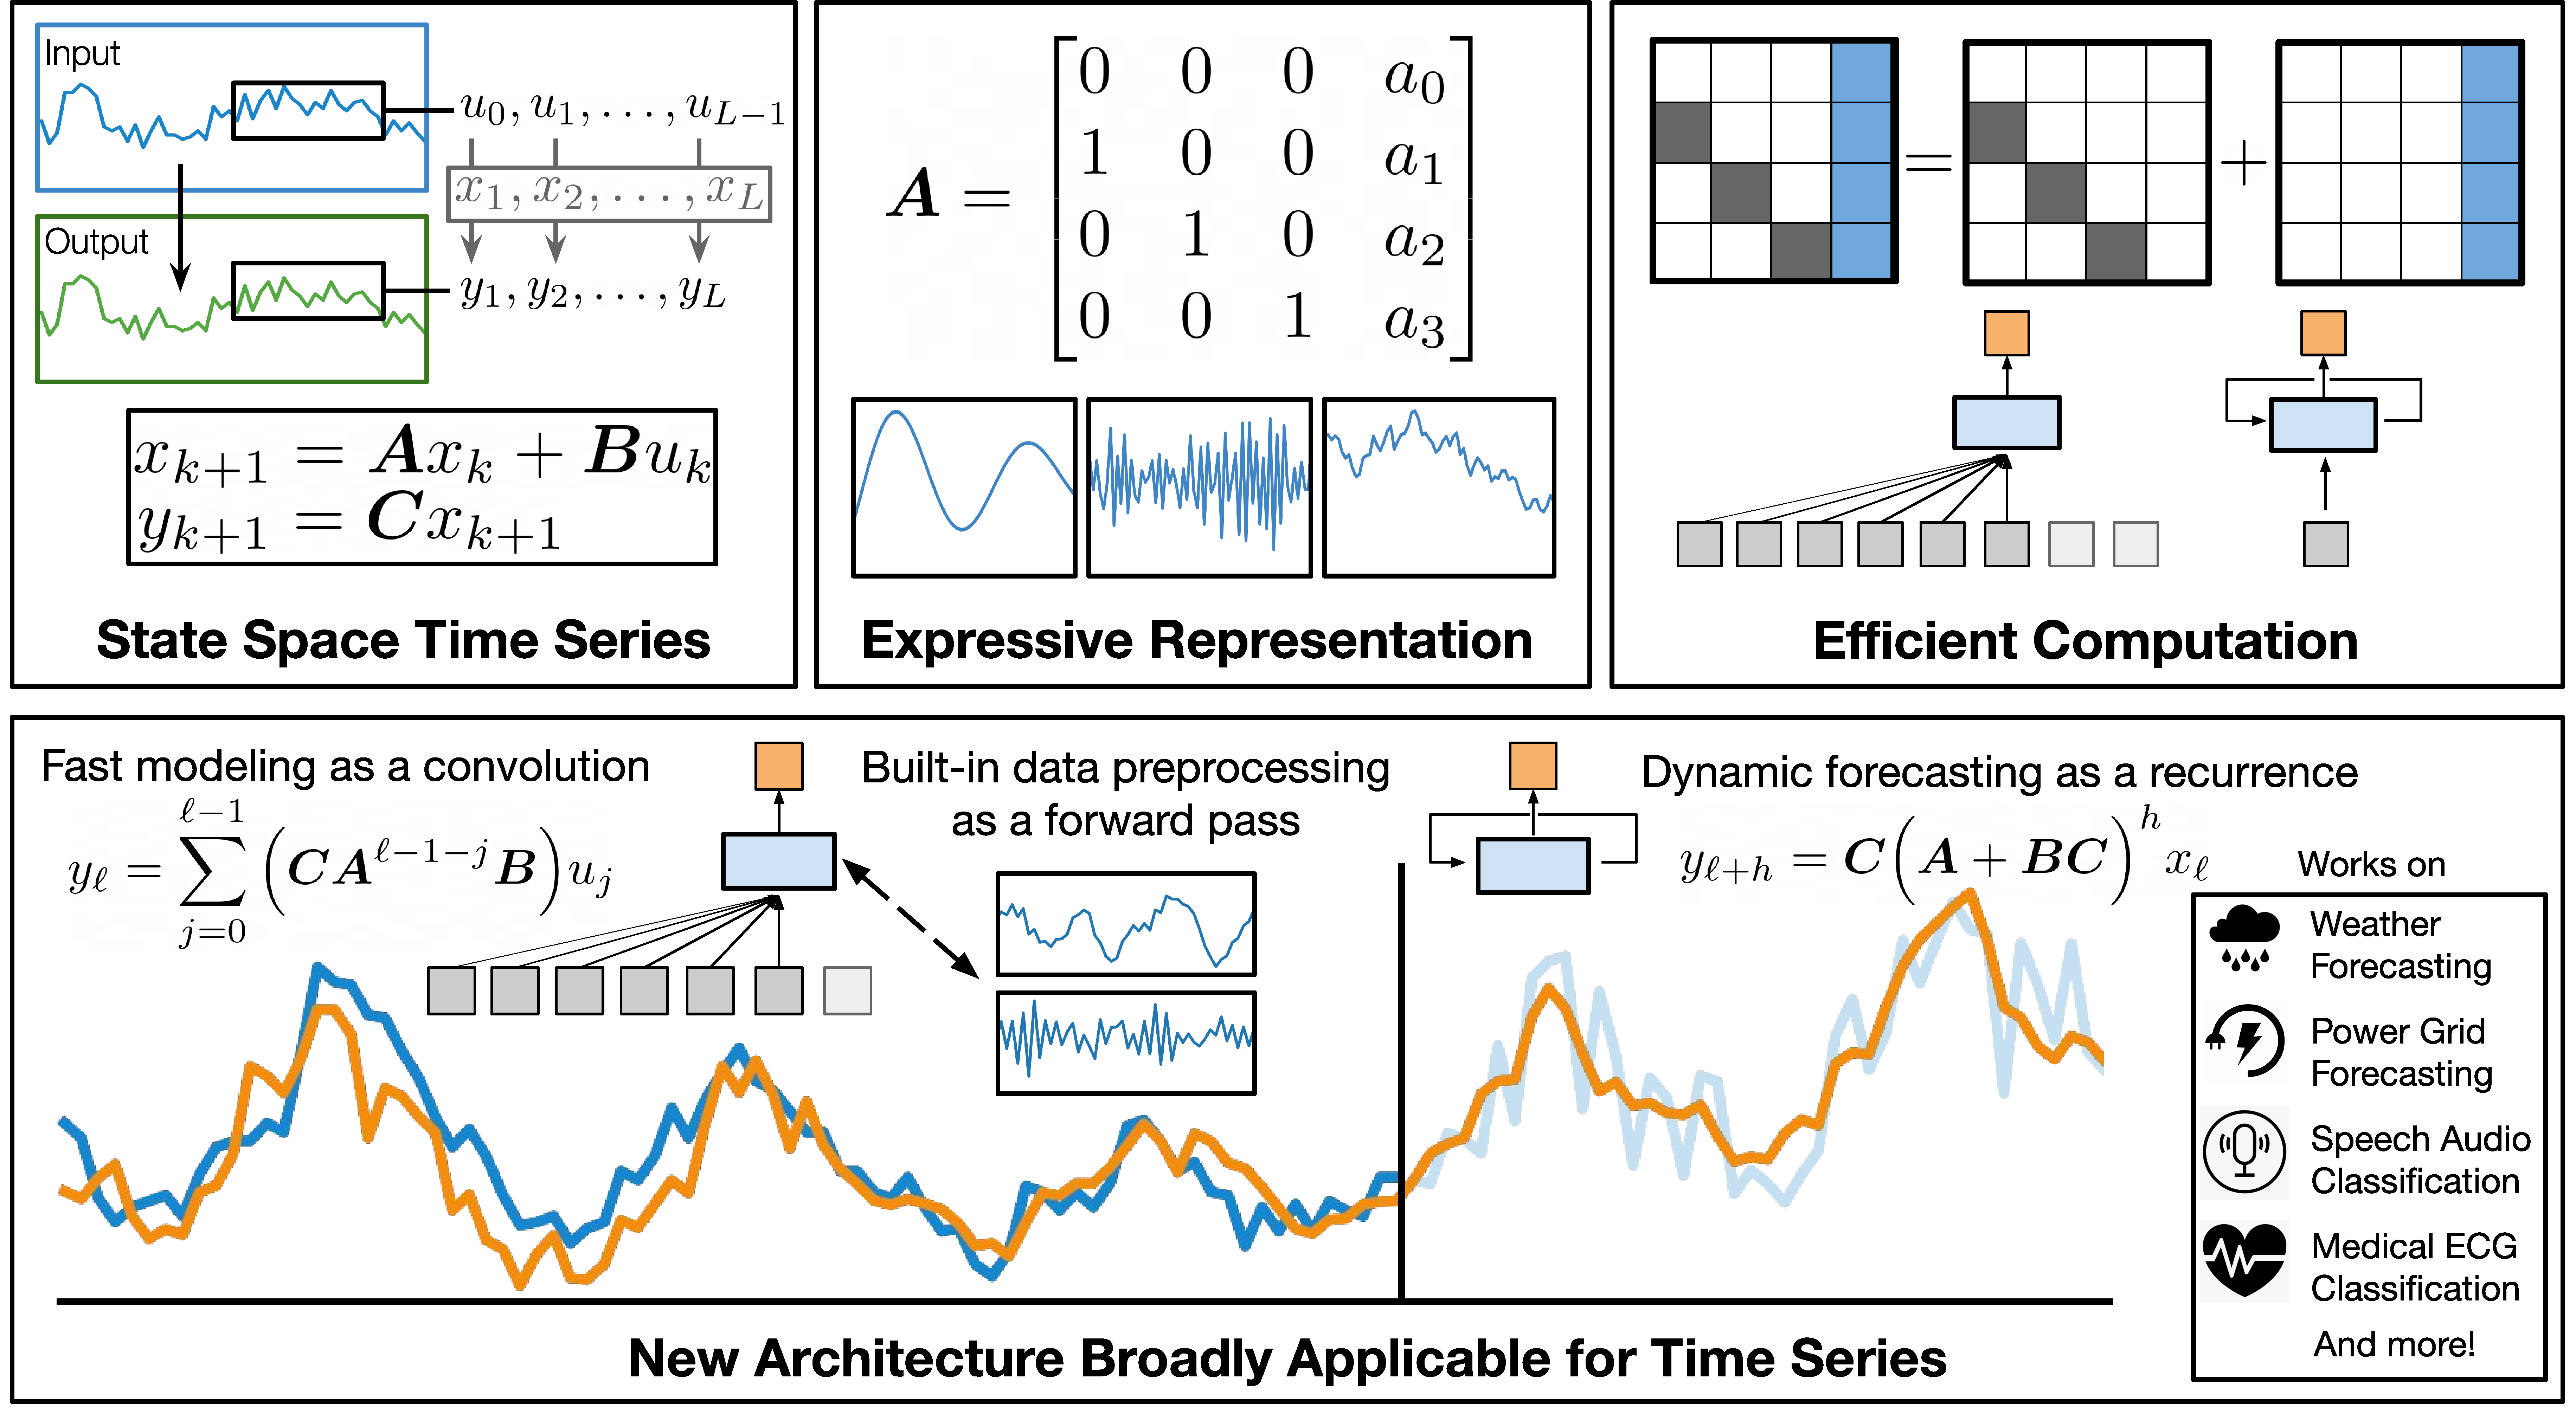
\includegraphics[width=1\textwidth]{_ICLR2023_paper/figures/time_series_ssm_use_this_2_levels_refactor1.pdf}
 \caption{We learn time series processes as state-space models (SSMs) (\textbf{top left}). We represent SSMs with the \textit{companion matrix}, which is a highly expressive representation for discrete time series  (\textbf{top middle}), and compute such SSMs efficiently as convolutions or recurrences via a shift + low-rank decomposition (\textbf{top right}). We use these SSMs to build \ourmethod{}, a new time series architecture broadly effective across tasks and domains (\textbf{bottom}).}
  \label{fig:overvew_fig1}
\end{figure}

% Our Method
%
% We thus propose \textbf{\ourmethod{}}, a new deep learning time series architecture. 
%
% Towards more effective time series modeling, 



We thus propose \textbf{\textsc{SpaceTime}}, a deep state-\textbf{space} architecture for effective \textbf{time} series modeling. 
% For more accurate forecasting and classification, 
To achieve this,
we focus on improving each criteria via three core contributions:

% \begin{enumerate}[itemsep=0.1pt,topsep=0pt,leftmargin=*]
\begin{enumerate}[topsep=0pt,leftmargin=*]
    \item For expressivity, our key idea and building block is a linear layer that models time series processes as \emph{state-space models} (SSMs) via the \emph{companion matrix} (Fig.~\ref{fig:overvew_fig1}). 
    We start with SSMs due to their connections to both classical time series analysis~\citep{kalman1960new, hamilton1994state} and recent deep learning advances~\citep{gu2021efficiently}. Classically, many time series models such as ARIMA and exponential smoothing (ETS) can be expressed as SSMs~\citep{box1970time, winters1960forecasting}. 
    Meanwhile, recent state-of-the-art deep sequence models~\citep{gu2021efficiently} have used SSMs to outperform Transformers and LSTMs on challenging long-range benchmarks~\citep{tay2020long}.
    % Meanwhile, recent SSM-based deep learning models~\citep{gu2021efficiently} have achieved state-of-the-art sequence modeling on challenging long-range benchmarks~\citep{tay2020long}. 
    Their primary innovations show how to formulate SSMs as neural network parameters that are practical to train. However, we find limitations with these deep SSMs for time series data. While we build on their advances, we prove that these prior SSM representations~\citep{ gu2021combining, gu2021efficiently, gupta2022diagonal}
    % cite these later: rangapuram2018, salinas2020deepar, lin2021ssdnet,
    cannot capture autoregressive processes fundamental for time series. We thus specifically propose the companion matrix representation for its expressive and memory-efficient properties. 
    We prove that the companion matrix SSM recovers fundamental autoregressive (AR) and smoothing processes modeled in classical techniques such as ARIMA and ETS, while only requiring $\mathcal{O}(d)$ memory to represent an $\mathcal{O}(d^2)$ matrix. 
    Thus, \ourmethod{} inherits the benefits of prior SSM-based sequence models, while introducing improved expressivity that 
    recovers fundamental time series processes
    % apture multiple AR processes and data preprocessing techniques 
    simply through its layer weights. 
    
    \item 
    % For forecasting over long horizons, we introduce a new ``closed-loop'' view of SSMs. Previous architectures apply the SSM in an ``open-loop'' fashion \citep{gu2021efficiently}, where the output is driven by the input sequence. 
    % However, to continuously forecast to long horizons, we require that the SSM has the ability to continue forecasting the signal in the absence of an input at those time steps. 
    % Inspired by classical closed-loop control~\citep{doyle2013feedback,aastrom2021feedback}, we propose a new variant of SSMs that explicitly models the next time-step input, which enables a multi-layer \ourmethod{} network to recurrently output long horizons.
    For forecasting long horizons, we introduce a new ``closed-loop'' view of SSMs. Prior deep SSM architectures either apply the SSM as an ``open-loop'' \citep{gu2021efficiently}, where fixed-length inputs necessarily generate same-length outputs, or use closed-loop autoregression where final layer outputs are fed through the \emph{entire} network as next-time-step inputs~\citep{goel2022s}. 
    We describe issues with both approaches in Sec.~\ref{sec:forecasting_ssm}, and instead achieve autogressive forecasting in a deep network with only a single SSM layer. We do so by explicitly training the SSM layer to predict its next time-step \emph{inputs}, alongside its usual outputs. This allows the SSM to recurrently generate its own future inputs that lead to desired outputs---\ie{} those that match an observed time series---so we can forecast over many future time-steps without explicit data inputs. 
    % This allows \ourmethod{} to generate its own final-layer inputs for outputting forecasts over many future time-steps.

    \item For efficiency, we introduce an algorithm for efficient training and inference with the companion matrix SSM. We 
    % first show how the companion SSM can be computed as both a convolution and a recurrence for layer-wise forward passes and forecasting respectively.  
    exploit the companion matrix's structure as a ``shift plus low-rank'' matrix, which allows us to reduce the time and space complexity for computing SSM hidden states and outputs from $\tilde{\mathcal{O}}(d \ell )$ to $\tilde{\mathcal{O}}(d + \ell)$ in SSM state size $d$ and input sequence length $\ell$. 
\end{enumerate}
% To subsequently build a full \ourmethod{} model, we simply stack together multiple layers---which each parametrize multiple companion matrix SSMs---into  a standard encoder-decoder architecture. 

% Simply stacking these layers together into a standard encoder-decoder architecture thus builds a highly expressive and efficient time series model.

In experiments, 
% we evaluate \ourmethod{} on extensive time series forecasting and classification tasks, and test if \ourmethod{}'s contributions empirically lead to (1) expressive time series modeling, (2) long-horizon forecasting, and (3) efficient training. 
%
we find \ourmethod{} consistently obtains state-of-the-art or near-state-of-the-art results, achieving best or second-best AUROC on 6 out of 7 ECG and audio speech time series classification tasks, and best mean-squared error (MSE) on 14 out of 16 Informer benchmark forecasting tasks~\citep{zhou2021informer}. \ourmethod{} also sets a new best average ranking across \numberMonashTasks{} tasks on the Monash benchmark~\citep{godahewa2021monash}.  
% 
We connect these gains with improvements on our three effective time series modeling criteria.  %
For expressivity, on synthetic ARIMA processes \ourmethod{} learns AR processes that prior deep SSMs cannot. 
%
% via extensive synthetics. As a controlled benchmark for expressiveness, we test how well popular architectures can fit standard AR processes, and find that \ourmethod{} best learns the true time series processes via its companion matrix SSM.
% compared to prior deep SSM representations.
%via visualizations of the process's ground-truth transfer function versus those parameterized by the trained SSM weights.
%
%
For long horizon forecasting, \ourmethod{} consistently outperforms prior state-of-the-art on the longest horizons by large margins. \ourmethod{} also generalizes better to \emph{new} horizons not used for training.
%
% validate that 
% We then validate (2) by showing that trained \ourmethod{}s generalize better to new horizons that models were not trained for. We also find that on the Informer benchmark, \ourmethod{} consistently outperforms alternatives on the longest evaluation horizons by the largest margins, up to $\textbf{X}$\% relative reduction in MSE for forecasting $\textbf{Y}$ time-steps.
%
% best RMSE on 25 out of 30 tasks from the diverse Monash benchmark~\citep{godahewa2021monash}.
% setting a new record among prior classical and deep learning approaches. 
% Moreover, we find that \ourmethod{} improves forecasts to arbitrary horizons (that it was not trained on) by \%XX on the Informer benchmark. 
For efficiency, on speed benchmarks \ourmethod{} obtains 73\% and 80\% relative wall-clock speedups over parameter-matched Transformers and LSTMs respectively, when training on real-world ETTh1 data.

% Discuss preliminaries for time series modeling? 
\section{Preliminaries}
%
% Should also discuss two kinds of forecasting?  
% \begin{itemize}
%     \item Iterated multi-step forecasting (IMS): Recursive and direct multi-step forecasting: the best of both worlds, volume 19 
%     \item Direct multi-step (DMS): Direct multi-step estimation and forecasting.
% \end{itemize}
% \subsection{Problem Setting}

\header{Problem setting} We evaluate effective time series modeling with
% In this work, we evaluate effective time series modeling with accurate 
classification and forecasting tasks. For both tasks, we are given input sequences of $\ell$ ``look-back'' or ``lag'' time series samples $\boldsymbol{u}_{t - \ell: t - 1} = (u_{t - \ell}, \ldots, u_{t - 1}) \in \mathbb{R}^{\ell \times m}$ for sample feature size $m$. 
%
For classification, we aim to classify the sequence as the true class $y$ out of  possible classes $\mathcal{Y}$. 
For forecasting, we aim to correctly predict $H$ future time-steps over a ``horizon'' $\boldsymbol{y}_{t, t + h - 1} = (u_{t}, \ldots, u_{t + h - 1}) \in \mathbb{R}^{h \times m}$.
% To do so, we require methods that are both expressive and efficient.

% \subsection{State-Space Models for Time Series}
\header{State-space models for time series} 
We build on the discrete-time state-space model (SSM), which maps observed inputs $u_k$ to hidden states $x_k$, before projecting back to observed outputs $y_k$
\begin{align}
    x_{k+1} &= \zA x_k + \zB u_k  \label{eq:discrete_ssm_state} \\
    y_k &= \zC x_k + \zD u_k \label{eq:discrete_ssm_output}
\end{align}
where $\zA\in\R^{d\times d}$, $\zB\in\R^{d \times m}$, $\zC\in\R^{m' \times d}$, and $\zD\in\R^{m' \times m}$. 
% where $\zA\in\R^{d\times d}$, $\zB\in\R^{d \times m}$, $\zC\in\R^{m \times d}$, and $\zD\in\R^{m \times m}$. 
%
% The same relationship specified by $A, B, C, D$ holds for all samples in the input sequence $\boldsymbol{u}$ and output sequence $\boldsymbol{y}$. 
% To model time series in the \emph{single} SSM setting, because data is typically given as a single sequence, we treat $\boldsymbol{u}$ and $\boldsymbol{y}$ as copies of the same time series sequence. 
% To model time series in the \emph{single} SSM setting, we treat $\boldsymbol{u}$ and $\boldsymbol{y}$ as copies of the same time series sequence, such that
For now,  
% standard linear dynamical systems conventions, 
we stick to \emph{single-input single-output} conventions where $m, m' = 1$, and let $\zD = 0$. 
%
To model time series in the single SSM setting, we treat $\boldsymbol{u}$ and $\boldsymbol{y}$ as copies of the same process, such that  
% \st{}
% Matrices $A, B, C$ thus govern how the time series evolves over time as
% % We use the conventional linear dynamical systems (LDS) notation also adopted in prior work~\citep{Brogan:226422, gu2021combining}. 
\begin{equation}
    y_{k + 1} = u_{k + 1} = \zC(\zA x_k + \zB u_k)
\label{eq:input_output_ts_equal}
\end{equation}
We can thus learn a time series SSM by treating $\zA, \zB, \zC$ as black-box parameters in a neural net layer, \ie{} by updating $\zA, \zB, \zC$ via gradient descent \st{} with input $u_k$ and state $x_k$ at time-step $k$, following (\ref{eq:input_output_ts_equal}) predicts $\hat{y}_{k + 1}$ that matches the next time-step sample $y_{k + 1} = u_{k + 1}$.
%
This SSM framework and modeling setup is similar to prior works~\citep{gu2021combining, gu2021efficiently}, which adopt a similar interpretation of inputs and outputs being derived from the ``same'' process, \eg{} for language modeling. Here we study and improve this framework for time series modeling.
%
As extensions, in Sec.~\ref{sec:expressive_ssm_with_companion} we show how (\ref{eq:discrete_ssm_state}) and (\ref{eq:discrete_ssm_output}) express univariate time series with the right $\zA$ representation.
% and generalize to multivariate time series in Sec.~\ref{sec:method_architecture_overview}. 
%
In Sec.~\ref{sec:method_spacetime_layer} we discuss the multi-layer setting, where layer-specific $\boldsymbol{u}$ and $\boldsymbol{y}$ now differ, and we only model first layer inputs and last layer outputs as copies of the same time series process.
% In Sec.~\ref{todo}, we show how we learn a time series SSM by treating $\zA, B, C$ as black-box parameters in a linear neural network layer, \ie{} by updating $\zA, B, C$ via gradient descent \st{} with input $u_k$ and state $x_k$ at time-step $k$, (\ref{eq:input_output_ts_equal}) results in prediction $\hat{y}_{k + 1}$ that matches the next time-step sample $y_{k + 1} = u_{k + 1}$. 

% predicting future samples from past samples, and training the SSM with a regression objective between the predicted and ground-truth outputs.
% via supervised regression between predicted outputs $\hat{\boldsymbol{y}} = \text{SSM}(\zu)$ and $\zy$.

% While \cite{gu2021combining} also model the continuous version of (\ref{eq:discrete_ssm_state}, \ref{eq:discrete_ssm_output}), we stick with the discrete SSM due to its relative simplicity, alignment with how time series data is often a discrete sequence, and expressive power.
% %
% In the next section, we expand on this last point. We introduce our specific formulation of $\zA$ as the companion matrix, and show how this enables learning expressive SSMs for a wide range of time series processes (which are not all learnable via prior continuous SSMs). 

% \header{Expressiveness}


% \subsection{Core Challenges for Effective Time Series Modeling}

% \header{Expressiveness}
% \MZ{
% Describe how we need to be able to capture higher-order dependencies. Need large enough model dimension size to do this. For example, DLinear does lag input size times prediction size. 
% }

% \header{Efficiency}
% \MZ{
% Discuss how we want to get to $O(D + L)$, but the naive solution is $O(DL)$. Describe why this is important for time-series (in order to actually learn higher-order and long-range dependencies, we need large enough dimension size for the model, and need to be able to process long enough sequence, with reasonable time-frame and memory size.

% For example, DLinear does lag input size times prediction size. This is not great, because you end up with a very big model where model parameters scale with the size of the input sequence and the horizon.  

% It's also not very robust to different timesteps? But we are more robust? 


% }
\section{Methodology}
\ours follows the same framework as speculative decoding, where each decoding step primarily consists of three substeps: (1) generating candidates, (2) processing candidates, and (3) accepting candidates. For \ours, (1) is achieved by \ours heads, (2) is realized by tree attention, and since \ours heads are on top of the original model, the logits calculated in (2) can be used for substep (1) for the next decoding step. The final step (3) can be realized by either rejection sampling~\citep{leviathan2022fast,chen2023accelerating} or typical acceptance (Section~\ref{sec:typical_acceptance}). The overall pipeline is illustrated in Figure~\ref{fig:pipeline}.

In this section, we first introduce the key components of \ours, including \ours heads, and tree attention. Then, we present two levels of fine-tuning procedures for \ours to meet the needs of different use cases. Finally, we propose two extensions to \ours, including self-distillation and typical acceptance, to handle situations where no training data is available for \ours and to improve the efficiency of the decoding process, respectively.
\subsection{Key Components}
\subsubsection{\ours Heads}
\label{sec:medusa_heads}
In speculative decoding, subsequent tokens are predicted by an auxiliary draft model. This draft model must be small yet effective enough to generate continuations that the original model will accept. Fulfilling these requirements is a challenging task, and existing approaches~\citep{spector2023accelerating,miao2023specinfer} often resort to separately \emph{pre-training} a smaller model. This pre-training process demands substantial additional computational resources. For example, in \citep{miao2023specinfer}, a reported 275 NVIDIA A100 GPU hours were used. Additionally, separate pre-training can potentially create a distribution shift between the draft model and the original model, leading to continuations that the original model may not favor. \citet{chen2023accelerating} have also highlighted the complexities of serving multiple models in a distributed environment.

\textcolor{black}{To streamline and democratize the acceleration of LLM inference, we take inspiration from \citet{stern2018blockwise}, which utilizes parallel decoding for tasks such as machine translation and image super-resolution. \ours heads}
 are additional decoding heads appended to the last hidden states of the original model. Specifically, given the original model's last hidden states $h_t$ at position $t$, we add $K$ decoding heads to $h_t$. The $k$-th head is used to predict the token in the $(t+k+1)$-th position of the next tokens (the original language model head is used to predict the $(t+1)$-th position). The prediction of the $k$-th head is denoted as $p_t^{(k)}$, representing a distribution over the vocabulary, while the prediction of the original model is denoted as $p_t^{(0)}$. Following the approach of \citet{stern2018blockwise}, we utilize a single layer of feed-forward network with a residual connection for each head. We find that this simple design is sufficient to achieve satisfactory performance. The definition of the $k$-th head is outlined as:

\begin{align*}
p_t^{(k)} = \text{softmax}\left(W_2^{(k)} \cdot \left(\text{SiLU}(W_1^{(k)} \cdot h_t)+h_t\right)\right),\\
\text{where } W_2^{(k)}\in\mathbb{R}^{d\times V}, W_1^{(k)}\in\mathbb{R}^{d\times d}.
\end{align*}

\textcolor{black}{$d$ is the output dimension of the LLM's last hidden layer and $V$ is the vocabulary size.}
\textcolor{black}{We initialize $W_2^{(k)}$ identically to the original language model head, and $W_1^{(k)}$ to zero.}
This aligns the initial prediction of \ours heads with that of the original model. The SiLU activation function~\citep{elfwing2017sigmoidweighted} is employed following the Llama models~\citep{touvron2023llama}.

Unlike a draft model, \ours heads are trained in conjunction with the original backbone model, which can remain \emph{frozen} during training (\ours-1) or be trained together (\ours-2). This method allows for fine-tuning large models even on a single GPU, taking advantage of the powerful base model's learned representations. Furthermore, it ensures that the distribution of the \ours heads aligns with that of the original model, thereby mitigating the distribution shift problem. Additionally, since the new heads consist of just a single layer akin to the original language model head, \ours does not add complexity to the serving system design and is friendly to distributed settings. We will discuss the training recipe for \ours heads in Section~\ref{sec:training_recipe}.

\subsubsection{Tree Attention}
\label{sec:tree_attention}
Through \ours heads, we obtain probability predictions for the subsequent $K+1$ tokens. These predictions enable us to create length-$K+1$ continuations as candidates. While the speculative decoding studies~\citep{leviathan2022fast,chen2023accelerating} suggest sampling a single continuation as the candidate, leveraging multiple candidates during decoding can enhance the expected acceptance length within a decoding step. Nevertheless, more candidates can also raise computational demands. To strike a balance, we employ a tree-structured attention mechanism to process multiple candidates concurrently.
\begin{figure}[ht]
    \centering
    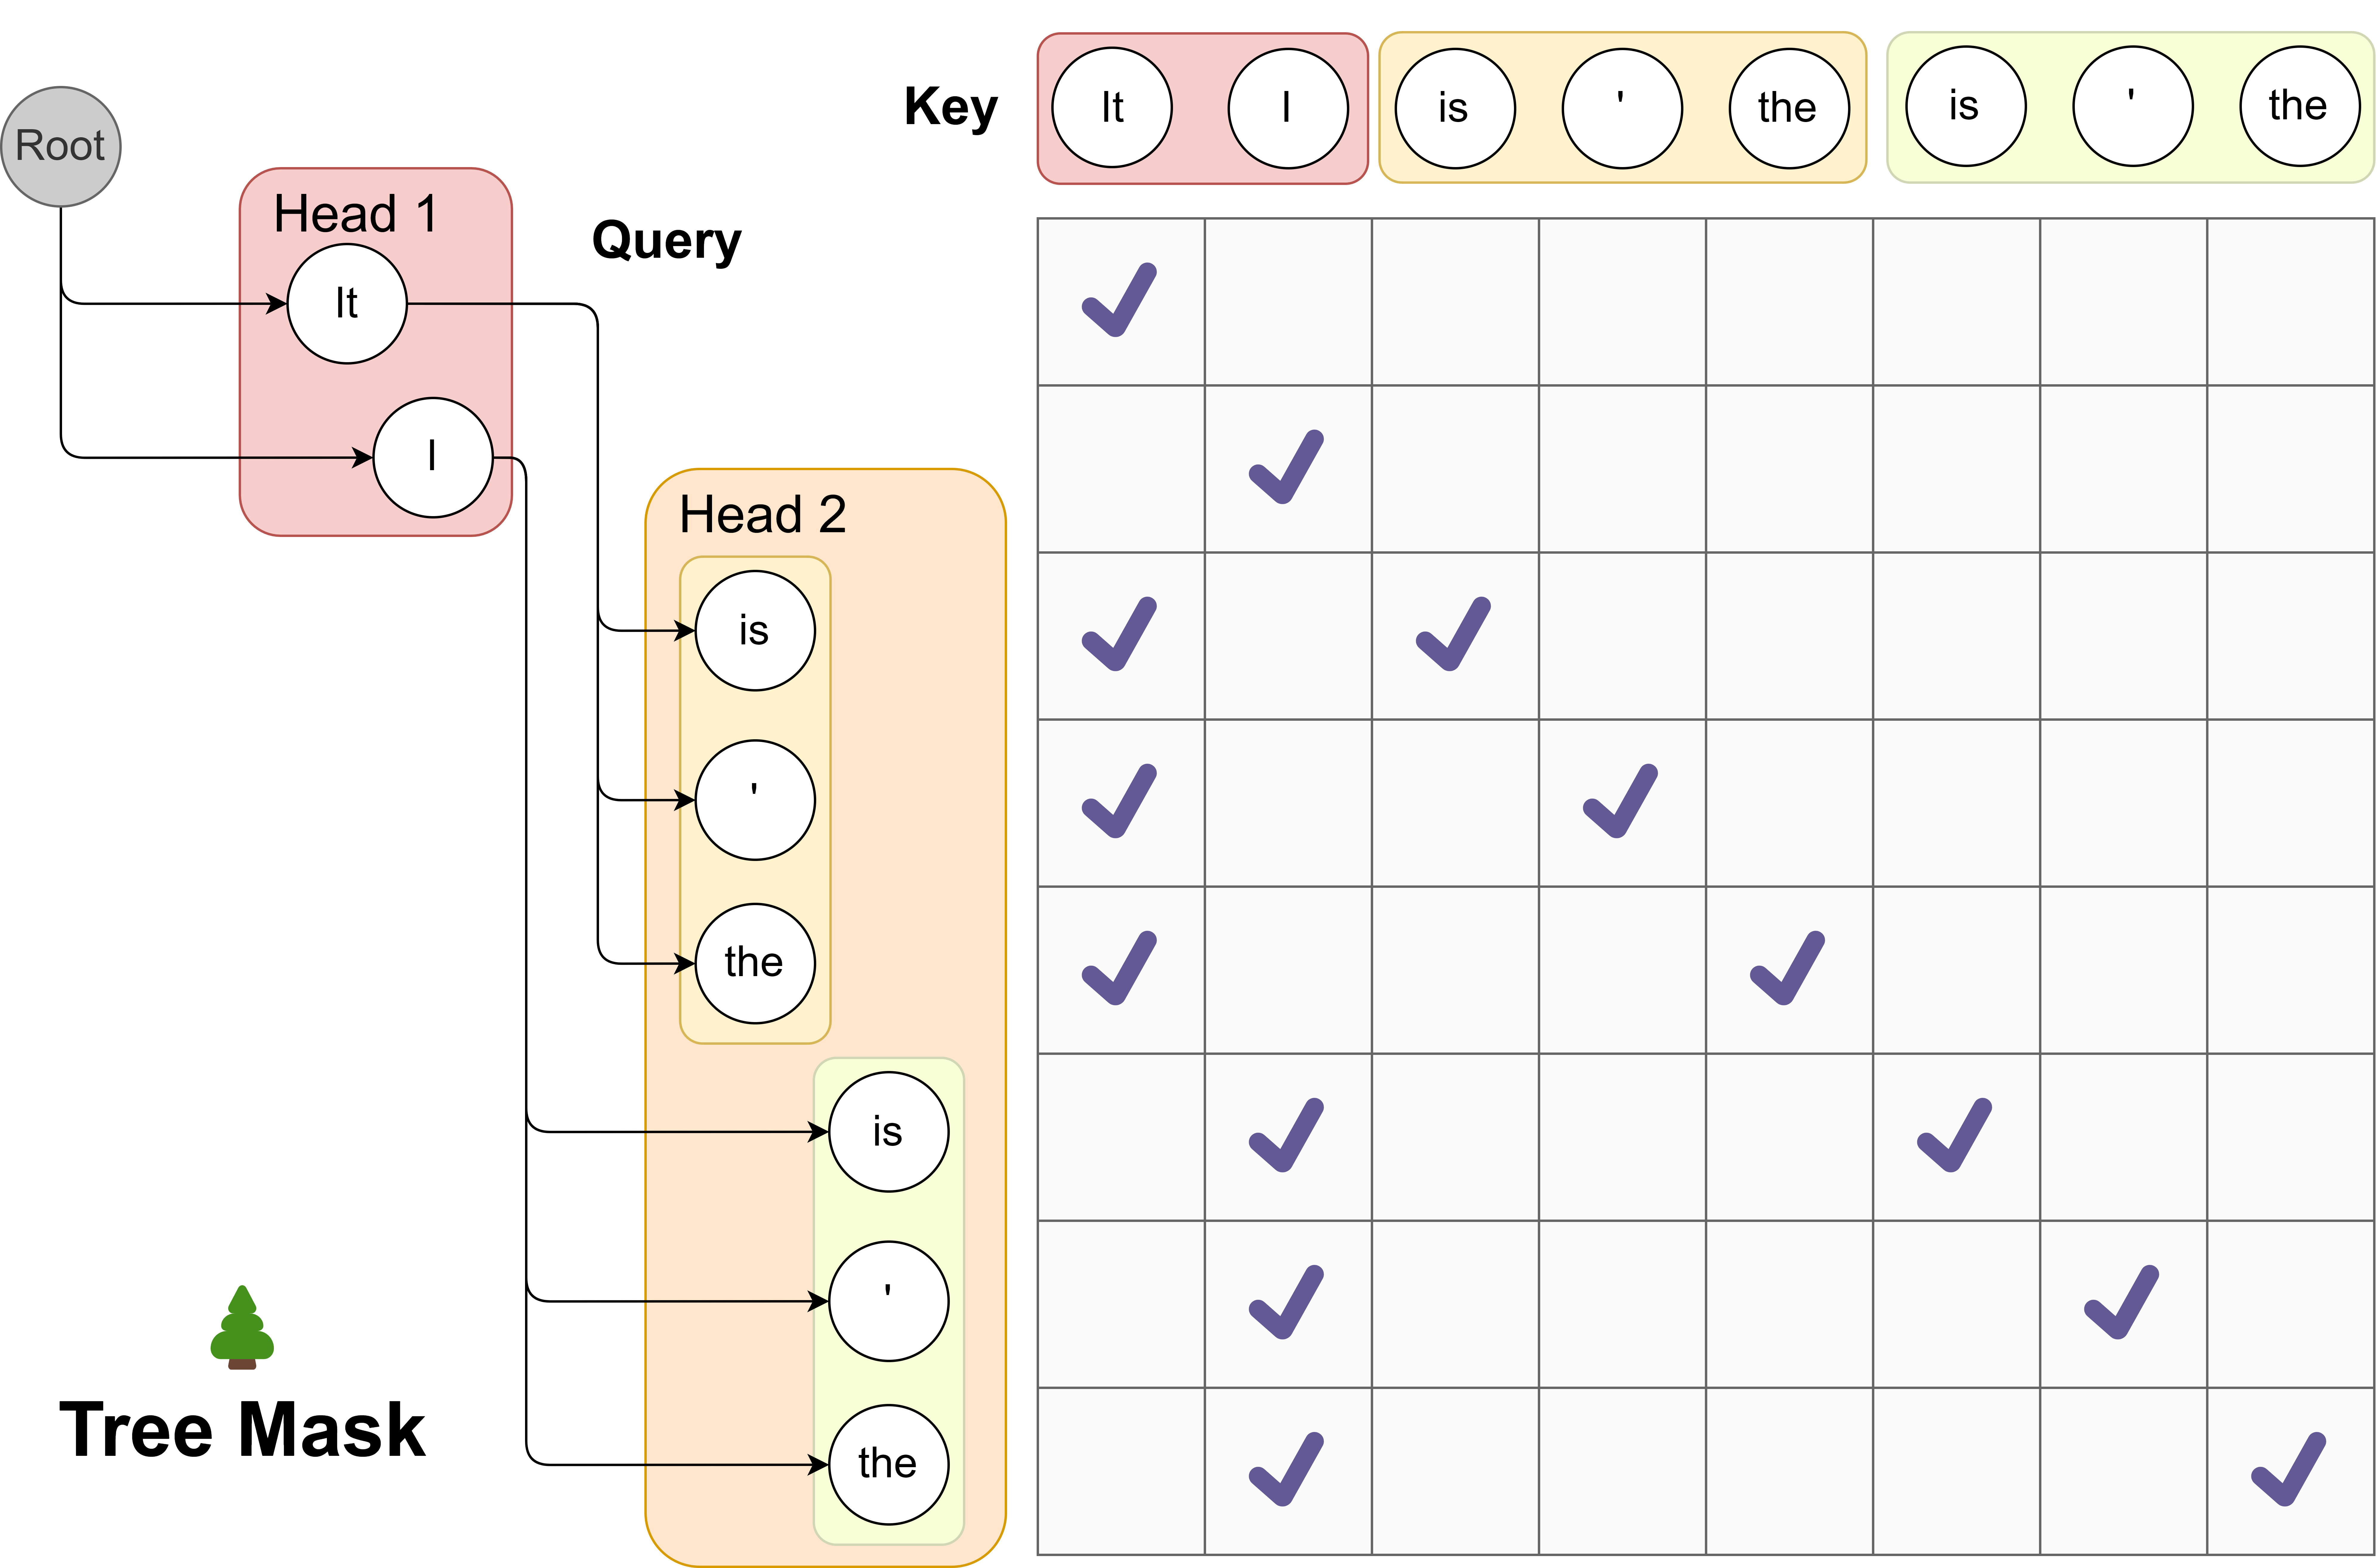
\includegraphics[width=0.45\textwidth]{tree_attention.png}
    \caption{
    We demonstrates the use of tree attention to process multiple candidates concurrently. As exemplified, the top-2 predictions from the first \ours head and the top-3 from the second result in a total of $2\times3=6$ candidates. Each of these candidates corresponds to a distinct branch within the tree structure. To guarantee that each token only accesses its predecessors, we devise an attention mask that exclusively permits attention flow from the current token back to its antecedent tokens. The positional indices for positional encoding are adjusted in line with this structure.}
    \label{fig:tree_attention}
\end{figure}
This attention mechanism diverges from the traditional causal attention paradigm. Within this framework, only tokens from the same continuation are regarded as historical data. Drawing inspiration from the concept of embedding graph structures into attention as proposed in the graph neural network domain~\citep{ying2021transformers}, we incorporate the tree structure into our attention mask, visualized in Figure~\ref{fig:tree_attention}. Remarkably, similar ideas have also been explored in independent works like \citet{miao2023specinfer,spector2023accelerating}, where they follow a bottom-up approach and construct the tree by merging multiple candidates generated by a draft model. In our method, we instead take a top-down approach to build the tree thanks to the structure of candidates generated by \ours heads. For a given $k$-th head, its top-$s_k$ predictions serve as the basis for candidate formation, where $s_k$ is a designated hyperparameter. These candidates are established by determining the Cartesian product of the top-$s_k$ predictions from each head. For instance, in Figure~\ref{fig:tree_attention}, with $s_1=2$ and $s_2=3$, each first head prediction can be succeeded by any prediction from the second head. This leads to a tree structure where $s_k$ branches exist at the $k$-th level (considering a virtual root as the $0$-level, in practice, this $0$-level is for the prediction of the language model head of the original model, which can be sampled independently). Within this tree, only a token's predecessors are seen as historical context, and our attention mask ensures that the attention is only applied on a token's predecessors. By employing this mask and properly setting the positional indices for positional encoding, we can process numerous candidates simultaneously without the need to expand the batch size. The cumulative number of new tokens is calculated as $\sum_{k=1}^K \prod_{i=1}^k s_i$.

In this section, we demonstrate the most simple and regular way to construct the tree structure by taking the Cartesian product. However, it is possible to construct the tree structure in a more sophisticated way and exploit the unbalanced accuracy of different top predictions of different heads. We will discuss this in Section~\ref{sec:optimized_tree_construction}.
\subsection{Training Strategies}
\label{sec:training_recipe}
At the most basic level, we can train \ours heads by freezing the backbone model and fine-tuning \ours heads. However, training the backbone in conjunction with the \ours heads can significantly enhance the accuracy of the \ours heads. Depending on the computational resources and the specific reqirements of the use case, we propose two levels of training strategies for \ours heads.

In this section, we assume the availability of a training dataset that aligns with the target model’s output distribution. This could be the dataset used for Supervised Fine-Tuning (SFT) of the target model. We will discuss eliminating the need for such a dataset using a self-distillation approach in Section~\ref{sec:self_distillation}.
\subsubsection{\ours-1: Frozen Backbone}
\label{sec:frozen_backbone}
To train \ours heads with a frozen backbone model, we can use the cross-entropy loss between the prediction of \ours heads and the ground truth. Specifically, given the ground truth token $y_{t+k+1}$ at position $t+k+1$, the loss for the $k$-th head is $\mathcal{L}_k = -\log p_t^{(k)}(y_{t+k+1})$ where $p_t^{(k)}(y)$ denotes the probability of token $y$ predicted by the $k$-th head. We also observe that $\mathcal{L}_k$ is larger when $k$ is larger, which is reasonable since the prediction of the $k$-th head is more uncertain when $k$ is larger. Therefore, we can add a weight $\lambda_k$ to $\mathcal{L}_k$ to balance the loss of different heads. And the total \ours loss is:
\begin{align}
    \label{eq:loss_medusa_1}
    \mathcal{L}_{\text{\ours-1}} = \sum_{k=1}^K -\lambda_k\log p_t^{(k)}(y_{t+k+1}).
\end{align}

In practice, we set $\lambda_k$ as the $k$-th power of a constant like $0.8$. Since we only use the backbone model for providing the hidden states, we can use a quantized version of the backbone model to reduce the memory consumption. This introduces a more democratized way to accelerate LLM inference, as with the quantization, \ours can be trained for a large model on a single consumer GPU similar to QLoRA~\citep{dettmers2023qlora}. The training only takes a few hours (e.g., 5 hours for \ours-1 on Vicuna 7B model with a single NVIDIA A100 PCIE GPU to train on 60k ShareGPT samples).
\subsubsection{\ours-2: Joint Training}
\label{sec:joint_training}
To further improve the accuracy of \ours heads, we can train \ours heads together with the backbone model. However, this requires a special training recipe to preserve the backbone model's next-token prediction capability and output quality. To achieve this, we propose three strategies:
\begin{itemize}
    \item \textbf{Combined loss}: To keep the backbone model's next-token prediction capability, we need to add the cross-entropy loss of the backbone model $\mathcal{L}_{\text{LM}}=-\log p_t^{(0)}(y_{t+1})$ to the \ours loss. We also add a weight $\lambda_0$ to balance the loss of the backbone model and the \ours heads. Therefore, the total loss is:
    \begin{align}
        \label{eq:loss_medusa_2}
        \mathcal{L}_{\text{\ours-2}} = \mathcal{L}_{\text{LM}} + \lambda_0\mathcal{L}_{\text{\ours-1}}.
    \end{align}
    \item \textbf{Differential learning rates}: Since the backbone model is already well-trained and the \ours heads need more training, we can use separate learning rates for them to enable faster convergence of \ours heads while preserving the backbone model's capability.
    \item \textbf{Heads warmup}: Noticing that at the beginning of training, the \ours heads have a large loss, which leads to a large gradient and may distort the backbone model's parameters. Following the idea from \citet{kumar2022finetuning}, we can employ a two-stage training process. In the first stage, we only train the \ours heads as \ours-1. In the second stage, we train the backbone model and \ours heads together with a warmup strategy. Specifically, we first train the backbone model for a few epochs, then train the \ours heads together with the backbone model. Besides this simple strategy, we can also use a more sophisticated warmup strategy by gradually increasing the weight $\lambda_0$ of the backbone model's loss. We find both strategies work well in practice.
\end{itemize}
Putting these strategies together, we can train \ours heads together with the backbone model without hurting the backbone model's capability. Moreover, this recipe can be applied together with Supervised Fine-Tuning (SFT), enabling us to get a model with native \ours support.
\subsubsection{How to Select the Number of Heads}
Empirically, we found that five heads are sufficient at most. Therefore, we recommend training with five heads and referring to the strategy described in Section~\ref{sec:optimized_tree_construction} to determine the optimal configuration of the tree attention. With optimized tree attention, sometimes three or four heads may be enough for inference. In this case, we can ignore the redundant heads without overhead.

\subsection{Extensions}
\subsubsection{Typical Acceptance}
\label{sec:typical_acceptance}
In speculative decoding papers~\citep{leviathan2022fast,chen2023accelerating}, authors employ rejection sampling to yield diverse outputs that align with the distribution of the original model. However, subsequent implementations~\citep{gante2023assisted,spector2023accelerating} reveal that this sampling strategy results in diminished efficiency as the sampling temperature increases. Intuitively, this can be comprehended in the extreme instance where the draft model is the same as the original one\textcolor{black}{:} 
Using greedy decoding, all output of the draft model will be accepted, therefore maximizing the efficiency. 
Conversely, rejection sampling introduces extra overhead, as the draft model and the original model are sampled independently. Even if their distributions align perfectly, the output of the draft model may still be rejected.

However, in real-world scenarios, sampling from language models is often employed to generate diverse responses, and the temperature parameter is used merely to modulate the ``creativity'' of the response. Therefore, higher temperatures should result in more opportunities for the original model to accept the draft model's output. We ascertain that it is typically unnecessary to match the distribution of the original model. Thus, we propose employing a \emph{typical acceptance} scheme to select plausible candidates rather than using rejection sampling. This approach draws inspiration from truncation sampling studies~\citep{hewitt2022truncation} (refer to \textcolor{black}{Appendix}~\ref{sec:related_work} for an in-depth explanation). Our objective is to choose candidates that are \emph{typical}, meaning they are not exceedingly improbable to be produced by the original model. We use the prediction probability from the \emph{original model} as a natural gauge for this and establish a threshold based on the prediction distribution to determine acceptance. Specifically, given $x_1, x_2, \cdots, x_n$ as context, when evaluating the candidate sequence \textcolor{black}{$(x_{n+1}, x_{n+2}, \cdots, x_{n+K+1})$ }(composed by top predictions of the original language model head and \ours heads), we consider the condition
\begin{align*}
p_{\text{original}}(x_{n+k}|x_1, x_2, \cdots, x_{n+k-1}) > \\\min\rbr{\epsilon, \delta\exp\rbr{-H(p_{\text{original}}(\cdot|x_1, x_2, \cdots, x_{n+k-1}))}},
\end{align*}
where $H(\cdot)$ denotes the entropy function, and $\epsilon, \delta$ are \textcolor{black}{the hard threshold and the entropy-dependent
threshold respectively}. This criterion is adapted from \citet{hewitt2022truncation} and rests on two observations: (1) tokens with relatively high probability are meaningful, and (2) when the distribution's entropy is high, various continuations may be deemed reasonable. During decoding, every candidate is evaluated using this criterion, and a \emph{prefix} of the candidate is accepted if it satisfies the condition. To guarantee the generation of at least one token at each step, we apply \emph{greedy decoding} for the first token and \emph{unconditionally} accept it while employing typical acceptance for subsequent tokens. The final prediction for the current step is determined by the \emph{longest accepted prefix} among all candidates.

Examining this scheme leads to several insights. Firstly, when the temperature is set to $0$, it reverts to greedy decoding, as only the most probable token possesses non-zero probability. As the temperature surpasses $0$, the outcome of greedy decoding will consistently be accepted with appropriate $\epsilon, \delta$, since those tokens have the maximum probability, yielding maximal speedup. Likewise, in general scenarios, an increased temperature will correspondingly result in longer accepted sequences, as corroborated by our experimental findings.

Empirically, we verify that typical acceptance can achieve a better speedup while maintaining a similar \textcolor{black}{generation quality} as shown in Figure~\ref{fig:threshold_ablation}.
\subsubsection{Self-Distillation}
\label{sec:self_distillation}
In Section~\ref{sec:training_recipe}, we assume the existence of a training dataset that matches the target model's output distribution. However, this is not always the case. For example, the model owners may only release the model without the training data, or the model may have gone through a Reinforcement Learning with Human Feedback (RLHF) procedure, which makes the output distribution of the model different from the training dataset. To tackle this issue, we propose an automated self-distillation pipeline to use the model itself to generate the training dataset for \ours heads, which matches the output distribution of the model.

The dataset generation process is straightforward. We first take a public seed dataset from a domain similar to the target model; for example, using the ShareGPT~\citep{sharegpt2023} dataset for chat models. Then, we simply take the prompts from the dataset and ask the model to reply to the prompts. In order to obtain multi-turn conversation samples, we can sequentially feed the prompts from the seed dataset to the model. Or, for models like Zephyr 7B~\citep{tunstall2023zephyr}, which are trained on both roles of the conversation, they have the ability to self-talk, and we can simply feed the first prompt and let the model generate multiple rounds of conversation.

For \ours-1, this dataset is sufficient for training \ours heads. However, for \ours-2, we observe that solely using this dataset for training the backbone and \ours heads usually leads to a lower generation quality. In fact, even without training \ours heads, training the backbone model with this dataset will lead to performance degradation. This suggests that we also need to use the original model's probability prediction instead of using the ground truth token as the label for the backbone model, similar to classic knowledge distillation works~\citep{kim2016sequencelevel}. Concretely, the loss for the backbone model is:
\begin{align*}
    \mathcal{L}_{\text{LM-distill}} = KL(p_{\text{original},t}^{(0)}||p_t^{(0)}),
\end{align*}
where $p_{\text{original},t}^{(0)}$ denotes the probability distribution of the original model's prediction at position $t$.

However, naively, to obtain the original model's probability prediction, we need to maintain two models during training, increasing the memory requirements. To further alleviate this issue, we propose a simple yet effective way to exploit the self-distillation setup. We can use a parameter-efficient adapter like LoRA~\citep{hu2021lora} for fine-tuning the backbone model. In this way, the original model is simply the model with the adapter turned off. Therefore, the distillation does not require additional memory consumption. Together, this self-distillation pipeline can be used to train \ours-2 without hurting the backbone model's capability and introduce almost no additional memory consumption. Lastly, one tip about using self-distillation is that it is preferable to use LoRA without quantization in this case, otherwise, the teacher model will be the quantized model, which may lead to a lower generation quality.

\subsubsection{Searching for the Optimized Tree Construction}
\label{sec:optimized_tree_construction}
In Section~\ref{sec:tree_attention}, we present the simplest way to construct the tree structure by taking the Cartesian product. However, with a fixed budget for the number of total nodes in the tree, a regular tree structure may not be the best choice. Intuitively, those candidates composed of the top predictions of different heads may have different accuracies. Therefore, we can leverage an estimation of the accuracy to construct the tree structure.

Specifically, we can use a calibration dataset and calculate the accuracies of the top predictions of different heads. Let $a_k^{(i)}$ denote the accuracy of the $i$-th top prediction of the $k$-th head\footnote{Here, the accuracy is defined for the single top $i$-th token, i.e., this accuracy is equal to top-$i$ accuracy minus top-$(i-1)$ accuracy.}. Assuming the accuracies are independent, we can estimate the accuracy of a candidate sequence composed by the top $\sbr{i_1, i_2, \cdots, i_k}$ predictions of different heads as $\prod_{j=1}^k a_j^{(i_j)}$. Let $I$ denote the set of all possible combinations of $\sbr{i_1, i_2, \cdots, i_k}$ and each element of $I$ can be mapped to a node of the tree (not only leaf nodes but all nodes are included). Then, the expectation of the acceptance length of a candidate sequence is:
\begin{align*}
    \sum_{\sbr{i_1, i_2, \cdots, i_k}\in I}\prod_{j=1}^k a_j^{(i_j)}.
\end{align*}
Thinking about building a tree by adding nodes one by one, the contribution of a new node to the expectation is exactly the accuracy associated with the node. Therefore, we can greedily add nodes to the tree by choosing the node that is connected to the current tree and has the highest accuracy. This process can be repeated until the total number of nodes reaches the desired number. In this way, we can construct a tree that maximizes the expectation of the acceptance length. Further details can be found in Appendix~\ref{appendix:sparse_tree}.


\vspace{-0.2cm}
\section{Experiments Details}
\label{sec:exp}

\vspace{-0.2cm}
\subsection{Roadmap Insights on FFHQ-256\texorpdfstring{~\cite{sg1}}{}}
\label{sub:arc-experiments}
\vspace{-0.1cm}
As per Table~\ref{tab:roadmap}, Config A (vanilla StyleGAN2) achieves an FID of 7.52 using the official implementation on FFHQ-256. Config B with all tricks removed achieves an FID of 12.46---performance drops as expected. 
Config C, with a well-behaved loss, achieves an FID of 11.65. But, now training is sufficiently stable to improve the architecture.

Config D, which improves $G$ and $D$ based on the classic ResNet and ConvNeXt findings, achieves an FID of 9.95. The output skips of the StyleGAN2 generator are no longer useful given our new architecture; including them produces a worse FID of 10.17. Karras~\etal find that the benefit of output skips is mostly related to gradient magnitude dynamics~\cite{sg3}, and this has been addressed by our ResNet architecture. For StyleGAN2, Karras~\etal conclude that a ResNet architecture is harmful to $G$~\cite{sg2}, but this is not true in our case as their ResNet implementation is considerably different from ours: 1) Karras~\etal use one 3-3 residual block for each resolution stage, while we have a separate transition layer and two 1-3-1 residual blocks; 2) i.3) and i.4) are violated as they do not have a linear residual block~\cite{mobnet} and the transition layer is placed on the skip branch of the residual block rather than the stem; 3) the essential principle of ResNet~\cite{resnet}---identity mapping~\cite{resnet2}---is violated as Karras~\etal divide the output of the residual block by $\sqrt{2}$ to avoid variance explosion due to the absence of a proper initialization scheme.

For Config E, we conduct two experiments that ablate i.\ref{item:i1} (increased width with depthwise conv.) and i.\ref{item:i2} (an inverted bottleneck). We add GroupedConv and reduce the bottleneck compression ratio to two given the same model size. Each bottleneck is now 1.5$\times$ the width of Config A, and the FID drops to 7.51, surpassing the performance of StyleGAN2. By inverting the stem and the bottleneck dimensions to enhance the capacity of GroupedConv, our final model achieves an FID of 7.05, exceeding StyleGAN2.


\begin{wraptable}[12]{r}{6.5cm}
\vspace{-1.25cm}
\centering
\caption{StackedMNIST 1000-mode coverage.}
% Our model outperforms other GANs in terms of $D_\text{KL}$, indicating that we are better able to recover the distribution.}
\vspace{-0.4cm}
\resizebox{0.8\linewidth}{!}{
\begin{tblr}{
  cell{2}{2} = {c},
  cell{2}{3} = {c},
  cell{3}{2} = {c},
  cell{3}{3} = {c},
  cell{4}{2} = {c},
  cell{4}{3} = {c},
  cell{5}{2} = {c},
  cell{5}{3} = {c},
  cell{6}{2} = {c},
  cell{6}{3} = {c},
  cell{7}{2} = {c},
  cell{7}{3} = {c},
  cell{8}{2} = {c},
  cell{8}{3} = {c},
  cell{9}{2} = {c},
  cell{9}{3} = {c},
  cell{10}{2} = {c},
  cell{10}{3} = {c},
  cell{11}{2} = {c},
  cell{11}{3} = {c},
  cell{12}{2} = {c},
  cell{12}{3} = {c},
  hline{2,12} = {1-3}{},
}
Model     & \# modes$\uparrow$ & $D_\text{KL}$$\downarrow$            &  \\
DCGAN~\cite{dcgan}     & 99            & 3.40\phantom{0}&  \\
VEEGAN~\cite{srivastava2017veegan}    & 150           & 2.95\phantom{0}&  \\
WGAN-GP~\cite{wgan-gp}& 959           & 0.73\phantom{0}&  \\
PacGAN~\cite{pacgan}    & 992           & 0.28\phantom{0}&  \\
StyleGAN2~\cite{sg2} & 940           & 0.42\phantom{0}&  \\
PresGAN~\cite{presgan}   & \textbf{1000} & 0.12\phantom{0}&  \\
Adv. DSM~\cite{advsm}  & \textbf{1000} & 1.49\phantom{0}&  \\
VAEBM~\cite{vaebm}     & \textbf{1000} & 0.087          &  \\
DDGAN~\cite{ddgan}     & \textbf{1000} & 0.071          &  \\
MEG~\cite{meg}       & \textbf{1000} & 0.031          &  \\
Ours---Config E     & \textbf{1000} & \textbf{0.029} &  
\end{tblr}
}
\label{tab:stackedmnist}
\end{wraptable}%

\subsection{Mode Recovery --- StackedMNIST\texorpdfstring{~\cite{metz2016unrolled}}{}} 
\vspace{-0.1cm}
We repeat the earlier experiment in 1000-mode convergence on StackedMNIST (unconditional generation), but this time with our updated architecture and with comparisons to SOTA GANs and likelihood-based methods (Tab.~\ref{tab:stackedmnist}, Fig.~\ref{fig:stacked-mnist}). 
One advantage brought up of likelihood-based models such as diffusion over GANs is that they achieve mode coverage~\cite{adm}. We find that most GANs struggle to find all modes. But, PresGAN~\cite{presgan}, DDGAN~\cite{ddgan}, and our approach are successful. Further, our method outperforms all other tested GAN models in term of KL divergence.

\subsection{FID --- FFHQ-256\texorpdfstring{~\cite{sg1}}{} (Optimized)}
\vspace{-0.1cm}
We train Config E model until convergence and with optimized hyperparameters and training schedule on FFHQ at 256$\times$256 (unconditional generation) (Tab.~\ref{tab:ffhq256}, Figs.~\ref{fig:ffhq-256-teaser} and~\ref{fig:ffhq-256}). 
Please see our supplemental material for training details.
%The hyperparameters and schedule are listed in the supplemental material. 
Our model outperforms existing StyleGAN methods, plus four more recent diffusion-based methods. On this common dataset experimental setting, many methods (not listed here) use the bCR~\cite{zhao2021improved} trick---this has only been shown to improve performance on FFHQ-256 (not even at different resolutions of FFHQ)~\cite{zhao2021improved, zhang2022styleswin}. We do not use this trick. 
% no such tricks in our method.
% JT Try to minimize embellishment...
% This is particularly impressive given the fact that the dataset FFHQ was designed for StyleGAN~\cite{sg1} and the StyleGAN series of models were optimized with this specific dataset in mind.
% to achieve this performance.

\subsection{FID --- FFHQ-64\texorpdfstring{~\cite{edm}}{}}
\vspace{-0.1cm}
To compare with EDM~\cite{edm} directly, we evaluate our model on FFHQ at 64$\times$64 resolution. For this, we remove the two highest resolution stages of our 256$\times$256 model, resulting in a generator that is less than half the number of parameters as EDM. Despite this, our model outperforms EDM on this dataset and needs one function evaluation only (Tab.~\ref{tab:ffhq64}).

\begin{figure}
\begin{floatrow}
    %\hspace{-0.75cm}%
    \capbtabbox{%
        \centering
        \resizebox{\linewidth}{!}{
        \begin{tblr}{
          column{2,3} = {r},
          cell{1}{2} = {c},
          cell{1}{3} = {c},
          hline{2,5,9,10} = {-}{},
        }
        Model       & NFE$\downarrow$ & FID$\downarrow$  \\
        StyleGAN2~\cite{sg2}   & 1               & 3.78 \\
        StyleGAN3-T~\cite{sg3} & 1               & 4.81 \\
        StyleGAN3-R~\cite{sg3} & 1               & 3.92 \\
        LDM~\cite{rombach2022high} & 200               & 4.98\\
        ADM (DDIM)~\cite{adm,compdiff} & 500               & 8.41\\
        ADM (DPM-Solver)~\cite{adm,compdiff} & 500               & 8.40\\
        Diffusion Autoencoder~\cite{diffae,compdiff} & 500               & 5.81\\
        Ours---Config E  & 1               & 2.75 \\
        \emph{With ImageNet feature leakage~\cite{kynkaanniemi2022role}:} & & \\
        PolyINR*~\cite{singh2023polynomial} & 1               & 2.72 \\
        StyleGAN-XL*~\cite{sgxl} & 1               & 2.19 \\
        StyleSAN-XL*~\cite{takida2024san} & 1               & 1.68 \\
        \end{tblr}
        }
    }{%
        \caption{
        \label{tab:ffhq256}FFHQ-256. * denotes models that leak ImageNet features.}
    }
    %
    \capbtabbox{%
        \centering
        \resizebox{0.85\linewidth}{!}{
        \begin{tblr}{
          column{2} = {r},
          column{3} = {r},
          hline{2,5,8} = {-}{},
        }
        Model         & NFE$\downarrow$ & FID$\downarrow$ \\
        StyleGAN2~\cite{sg2,anycostgan}     & 1               & 3.32            \\
        MSG-GAN~\cite{karnewar2020msg,anycostgan}       & 1               & 2.7             \\
        Anycost GAN~\cite{anycostgan}   & 1               & 2.52            \\
        VE~\cite{sde,edm}            & 79              & 25.95           \\
        VP~\cite{sde,edm}            & 79              & 3.39            \\
        EDM~\cite{edm}           & 79              & 2.39            \\
        Ours—Config E & 1               & 1.95 \\
        \end{tblr}
        }
    }{%
        \caption{\label{tab:ffhq64}FFHQ-64.}
    }
\end{floatrow}
\vspace{-0.25cm}
\end{figure}


% \begin{figure}
% \begin{floatrow}
%     \capbtabbox{%
%         \centering
%         \resizebox{0.8\linewidth}{!}{
%         \begin{tblr}{
%           column{2,3} = {r},
%           cell{1}{2} = {c},
%           cell{1}{3} = {c},
%           hline{2,9,13} = {-}{},
%         }
%         Model               & NFE$\downarrow$ & FID$\downarrow$ \\
%         BigGAN~\cite{biggan}              & 1               & 14.73 \\
%         TransGAN~\cite{trans}            & 1               & 9.26 \\
%         ViTGAN~\cite{vitgan}              & 1               & 6.66 \\
%         DDGAN~\cite{ddgan}               & 4               & 3.75 \\
%         Diffusion StyleGAN2~\cite{diffusiongan} & 1               & 3.19 \\
%         StyleGAN2 + ADA~\cite{sg2ada}     & 1               & 2.42 \\
%         StyleGAN3-R + ADA~\cite{sg3,studio}   & 1               & 10.83 \\
%         DDPM~\cite{ddpm}               & 1000            & 3.21 \\
%         DDIM~\cite{ddim}                & 50             & 4.67 \\
%         VE~\cite{sde,edm}                  & 35              & 3.11 \\
%         VP~\cite{sde,edm}                  & 35              & 2.48 \\
%         Ours---Config E     & 1               & 1.96 \\
%         \hline
%         \emph{With ImageNet feature leakage~\cite{kynkaanniemi2022role}:} & & \\
%         StyleGAN-XL*~\cite{sgxl}       & 1               & 1.85 \\
%         \end{tblr}
%         }
%     }{%
%         \caption{\label{tab:cifar10}CIFAR-10.}
%     }
%         % \begin{tblr}{
%         %   column{2,3} = {r},
%         %   cell{1}{2}{3} = {},
%         %   hline{2,9,13} = {-}{},
%         % }
%         % Model               & FID$\downarrow$ & Params          \\
%         % BigGAN~\cite{biggan}              & 14.73  & --       \\
%         % TransGAN~\cite{trans}            & 9.26 & --         \\
%         % ViTGAN~\cite{vitgan}              & 6.66 & --         \\
%         % DDGAN~\cite{ddgan}               & 3.75 & --         \\
%         % Diffusion StyleGAN2 & 3.19 & 40.1M           \\
%         % StyleGAN2 + ADA     & 2.42 & 40.1M          \\
%         % StyleGAN3-R + ADA   & 10.83 & 40.1M        \\
%         % DDPM               & 3.21 & 35.2M         \\
%         % DDIM                & 4.67 & --         \\
%         % VE~\cite{edm}                  & 3.11 & 61.8M        \\
%         % VP~\cite{edm}                  & 2.48 & 61.8M         \\
%         % Ours---Config E     & \textbf{1.99}  & 43.0M \\
%         % StyleGAN-XL*~\cite{sgxl}       & 	1.85 & 140.0M \\
%         % \end{tblr}
        
%     %     }
%     % }{%
%     %     \caption{\label{tab:cifar10}CIFAR-10.}
%     % }%
%     %\hspace{-0.75cm}%
%     %\hspace{-0.5cm}%
% \end{floatrow}
% \end{figure}

\subsection{FID --- CIFAR-10~\cite{krizhevsky2009learning}} \vspace{-0.1cm}

\begin{wraptable}[14]{r}{6.5cm}
\vspace{-0.75cm}
\centering
\caption{\label{tab:cifar10}CIFAR-10 performance.}
\vspace{-0.4cm}
\resizebox{0.9\linewidth}{!}{
    \begin{tblr}{
          column{2,3} = {r},
          cell{1}{2} = {c},
          cell{1}{3} = {c},
          hline{2,9,13} = {-}{},
        }
        Model               & NFE$\downarrow$ & FID$\downarrow$ \\
        BigGAN~\cite{biggan}              & 1               & 14.73 \\
        TransGAN~\cite{trans}            & 1               & 9.26 \\
        ViTGAN~\cite{vitgan}              & 1               & 6.66 \\
        DDGAN~\cite{ddgan}               & 4               & 3.75 \\
        Diffusion StyleGAN2~\cite{diffusiongan} & 1               & 3.19 \\
        StyleGAN2 + ADA~\cite{sg2ada}     & 1               & 2.42 \\
        StyleGAN3-R + ADA~\cite{sg3,studio}   & 1               & 10.83 \\
        DDPM~\cite{ddpm}               & 1000            & 3.21 \\
        DDIM~\cite{ddim}                & 50             & 4.67 \\
        VE~\cite{sde,edm}                  & 35              & 3.11 \\
        VP~\cite{sde,edm}                  & 35              & 2.48 \\
        Ours---Config E     & 1               & 1.96 \\
        \hline
        \emph{With ImageNet feature leakage~\cite{kynkaanniemi2022role}:} & & \\
        StyleGAN-XL*~\cite{sgxl}       & 1               & 1.85 \\
        \end{tblr}
}
\end{wraptable}

We train Config E model until convergence and with optimized hyperparameters and training schedule on CIFAR-10 (conditional generation) (Tab.~\ref{tab:cifar10}, Fig.~\ref{fig:cifar10}). Our method outperforms many other GANs by FID even though the model has relatively small capacity. For instance, StyleGAN-XL~\cite{sgxl} has 18\ M parameters in the generator and 125\ M parameters in the discriminator, while our model has a 40\ M parameters between the generator and discriminator combined (Fig.~\ref{fig:fid-50k-vs-params-cifar-10}). Compared to diffusion models like LDM or ADM, GAN inference is significantly cheaper as it requires only one network function evaluation compared to the tens or hundreds of network function evaluations for diffusion models without distillation. 

\begin{wrapfigure}[12]{r}{6.5cm}
    \vspace{-0.4cm}
    \centering
    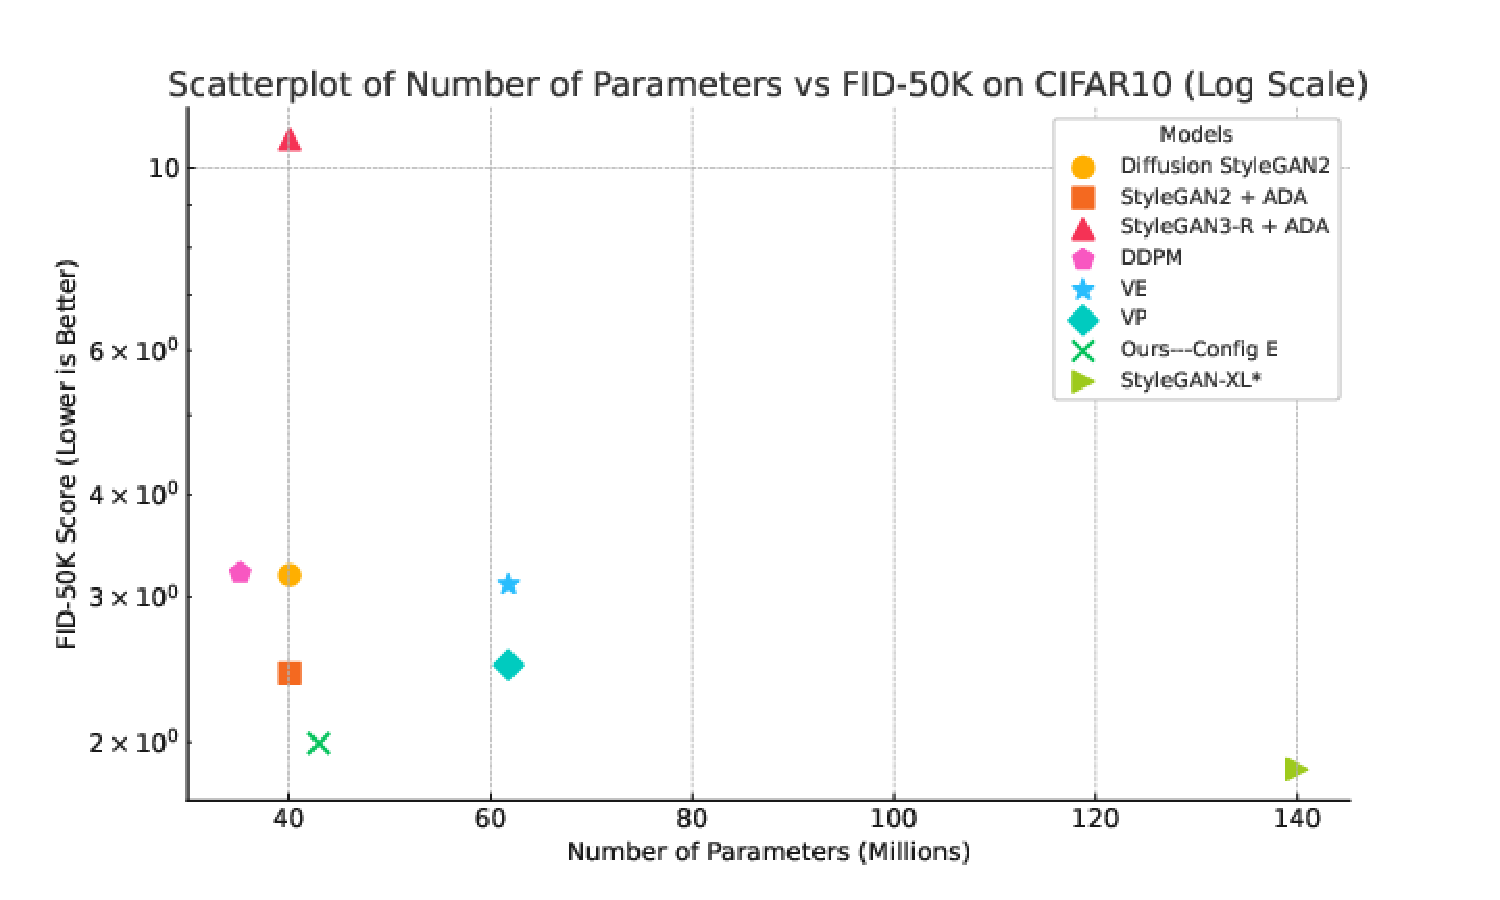
\includegraphics[width=\linewidth,clip,trim={0 0 0 2cm}]{figures/Scatterplot-FID-Parameters-CIFAR10.pdf}
    \caption{Millions of parameters vs.~FID-50K (log scale) on CIFAR-10. Lower is better.}
    \label{fig:fid-50k-vs-params-cifar-10}
\end{wrapfigure}

Many state-of-the-art GANs are derived from Projected GAN~\cite{sauer2021projected}, including StyleGAN-XL~\cite{sgxl} and the concurrent work of StyleSAN-XL~\cite{takida2024san}. These methods use a pre-trained ImageNet classifier in the discriminator. Prior work has shown that a pre-trained ImageNet discriminator can leak ImageNet features into the model~\cite{kynkaanniemi2022role}, causing the model to perform better when evaluating on FID since it relies on a pre-trained ImageNet classifier for the loss. But, this does not improve results in perceptual studies~\cite{kynkaanniemi2022role}. Our model produces its low FID without any ImageNet pre-training.

%\jt{Missing citations here for such methods.}


%\aaron{add NFEs}
%\jt{Which models in our evaluation use this? Any?}

%\jt{What is the second caveat?}

\subsection{FID --- ImageNet-32~\cite{chrabaszcz2017downsampled}}
\label{sec:imagenet32-fid-explain}
We train Config E model until convergence and with optimized hyperparameters and training schedule on ImageNet-32 (conditional generation). We compare against recent GAN models and recent diffusion models in Table~\ref{tab:imagenet32}.
We adjust the number of parameters in the generator of our model to match StyleGAN-XL~\cite{sgxl}'s generator (84M parameters). Specifically, we make the model significantly wider to match. Our method achieves comparable FID despite using a 60\% smaller discriminator (Tab.~\ref{tab:imagenet32}) and despite not using a pre-trained ImageNet classifier.
%, which has been shown to improve FID performance, but not improve results in perceptual studies~\cite{kynkaanniemi2022role}.

\vspace{-0.1cm}
\subsection{FID --- ImageNet-64~\cite{chrabaszcz2017downsampled}}
We evaluate our model on ImageNet-64 to test its scalability. We stack another resolution stage on our ImageNet-32 model, resulting in a generator of 104\ M parameters. This model is nearly 3$\times$ smaller than diffusion-like models~\cite{adm,edm,cm,icm} that rely on the ADM backbone, which contains about 300\ M parameters. Despite the smaller model size and that our model generates samples in one step, it outperforms larger diffusion models with many NFEs on FID (Tab.~\ref{tab:imagenet64}).

\vspace{-0.1cm}
\subsection{Recall}
We evaluate the recall~\cite{precrecall} of our model on each dataset to quantify sample diversity. In general, our model achieves a recall that is similar to or marginally worse than the diffusion model counterpart, yet superior to existing GAN models. For CIFAR-10, the recall of our model peaked at 0.57; as a point of comparison, StyleGAN-XL~\cite{sgxl} has a worse recall of 0.47 despite its lower FID. For FFHQ, we obtain a recall of 0.53 at 64$\times$64 and 0.49 at 256$\times$256, whereas StyleGAN2~\cite{sg2} achieved a recall of 0.43 on FFHQ-256. Our ImageNet-32 model achieved a recall of 0.63; comparable to ADM~\cite{adm}. Our ImageNet-64 model achieved recall 0.59. While this is slightly worse than $\approx$0.63 that many diffusion models achieve, it is better than BigGAN-deep~\cite{biggan} which achieved a recall of 0.48.

\begin{figure}
    \begin{floatrow}
        \capbtabbox{%
        \centering
        \resizebox{0.9\linewidth}{!}{
        \begin{tblr}{
          column{2} = {r},
          column{3} = {r},
          cell{8}{1} = {c=3}{},
          hline{2,7-8} = {-}{},
        }
    Model                                                       & NFE$\downarrow$  & FID$\downarrow$                        \\ 
    DDPM++~\cite{kim2021soft}                  & 1000 & 8.42                                   \\
    VDM~\cite{kingma2021variational}           & 1000 & 7.41                                   \\
    MSGAN~\cite{karnewar2020msg,ning2023input} & 1    & 12.3                                   \\
    ADM~\cite{adm}                             & 1000 & 3.60                                   \\
    DDPM-IP~\cite{ning2023input}               & 1000 & 2.87                                   \\
    Ours—Config E               & 1    & 1.27   \\
    \textit{With ImageNet feature leakage~\cite{kynkaanniemi2022role}:}    \\
    StyleGAN-XL*~\cite{sgxl}                   & 1    & 1.10                                  
    \end{tblr}
        }
    }{%
        \caption{\label{tab:imagenet32}ImageNet-32.}
        % \jt{some are conditional still}}
    }
    %
    \capbtabbox{
        \centering
        \resizebox{0.9\linewidth}{!}{
        \begin{tblr}{
          column{2} = {r},
          column{3} = {r},
          cell{1}{2} = {c},
          cell{1}{3} = {c},
          cell{12}{1} = {c=3}{},
          hline{2-3,11-12} = {-}{},
        }
        Model         & NFE$\downarrow$ & FID$\downarrow$ \\
        BigGAN-deep~\cite{biggan}\phantom{xx}   & 1               & 4.06            \\
        DDPM~\cite{ddpm}          & 250             & 11.0            \\
        DDIM~\cite{ddim}          & 50              & 13.7            \\
        ADM~\cite{adm}           & $^\S$250             & 2.91            \\
        EDM~\cite{edm}           & 79              & 2.23            \\
        CT~\cite{cm}            & 2               & 11.1            \\
        CD~\cite{cm}            & 3               & 4.32            \\
        iCT-deep~\cite{icm}      & 2               & 2.77            \\
        DMD~\cite{dmd}           & 1               & 2.62            \\
        Ours—Config E & 1               & 2.09            \\
        \emph{With ImageNet feature leakage~\cite{kynkaanniemi2022role}:}          &                 &                 \\
        StyleGAN-XL*~\cite{sgxl}   & 1               & 1.52            
        \end{tblr}
        }
    }
    {
        \caption{\label{tab:imagenet64}ImageNet-64.\hspace{-0.1cm} {\small \S:\hspace{-0.05cm}deterministic sampling.}}
    }
    \end{floatrow}
    \vspace{-0.25cm}
\end{figure}


% \begin{table}[ht]
%     \centering
%     \begin{tabular}{lcccccccc}
%         \toprule
%         \textbf{Model} & \textbf{\# Param.} & \textbf{IS $\uparrow$} & \textbf{FID $\downarrow$} & \textbf{Precision $\uparrow$} & \textbf{Recall $\uparrow$} & \textbf{Density $\uparrow$} & \textbf{Coverage $\uparrow$} & \textbf{Inf. (s)} \\
%         \midrule
%         ReACGAN + DiffAug (Ours) [10] & 9.4M & 10.15 & 2.64 & 0.75 & 0.65 & 0.98 & 0.90 & 0.009 \\
%         StyleGAN2-ADA [85] & 20.2M & 10.31 & 2.41 & 0.74 & 0.68 & 1.02 & 0.92 & 0.008 \\
%         StyleGAN2-ADA (Ours) [85] & 20.2M & \textbf{10.53} & 2.31 & 0.75 & 0.69 & 1.04 & 0.93 & 0.008 \\
%         StyleGAN2 + DiffAug + D2D-CE (Ours) [10] & 20.2M & 10.46 & 2.30 & 0.76 & 0.68 & 1.03 & 0.93 & 0.007 \\
%         DDPM [43] & 35.2M & 9.73 & 3.23 & 0.78 & 0.67 & 1.10 & 0.93 & 15.422 \\
%         DDPM++ [44] & 106.6M & 9.90 & 2.49 & 0.78 & 0.69 & 1.12 & 0.94 & 46.697 \\
%         NCSN++ [44] & 107.6M & 10.08 & 2.27 & 0.77 & 0.70 & 1.07 & 0.94 & 99.304 \\
%         LSGM [45] & - & 10.04 & 2.80 & 0.80 & 0.70 & 1.15 & 0.95 & - \\
%         LSGM-ODE [45] & - & 10.07 & \textbf{2.09} & 0.77 & 0.71 & 1.03 & 0.94 & - \\
%         CLD-SGM [47] & - & 9.88 & 2.38 & 0.78 & 0.69 & 1.12 & 0.94 & - \\
%         StyleGAN-XL~ & 18.0M & \textbf{11.03} & \textbf{1.88} & 0.77 & 0.59 & 1.08 & 0.94 & 0.010 \\
%         % BaselineGAN & %10.284011840820312
%         % 10.28
%         % & %1.9925376117527978 
%         % 1.99 & % 0.6899600028991699 
%         % 0.69 &&
%         \bottomrule
%     \end{tabular}
%     \caption{Comparison of various models on CIFAR10 dataset. TODO fix citation}
% \label{tab:cifar10_comparison}
%\end{table}

% \jt{Is the below meant to be a conclusion? Some of these statements are unfounded in the evidence we present so far.}
% \begin{enumerate}

%     \item We demonstrate the ability of our method to recover all modes of training data on Stacked Mnist~\ref{tab:stackedmnist}.
%     \item We beat all methods that do not use bCR (shown to overfit for FFHQ-256~\cite{}) and methods that do not leak imagenet features from a pretrained discriminator~\cite{kynkaanniemi2022role}. If we exclude these two categories of models, we are SOTA across all open source GANs. We also SOTA on a per parameter count basis on multiple GANs.
%     \item We demonstrate SOTA performance on CIFAR-10 image generation at our current parameter count, outperforming all previous GANs except for StyleGAN-XL derived ones with X\% percent of the parameters of these methods. We also do not leak features from ImageNet or use a pretrained discriminator.~\ref{tab:cifar10}. 
%     \item We achieve near SOTA on FFHQ 256 and achieve SOTA for a GAN method without bCR or feature leakage.
%     \item We achieve near state of the art results on Imagenet and achieve Pareto frontier results for total GAN model parameter size.
% \end{enumerate}
% \begin{table}[h]
\centering
\caption{FID on ImageNet-32}
\begin{tabular}{ l c c }
\toprule
Model & \textbf{Year} & FID$\downarrow$ \\
\midrule
% %Real NVP (Dinh et al.) & 2016 & 4.28 \\
% %Glow (Kingma and Dhariwal) & 2018 & 4.09 \\
% %MintNet & 2019 & 4.06 \\
% % Residual Flow & 2019 & 4.01 \\
% % BIVA Maaloe et al. & 2019 & 3.96 \\
% % ANF Huang et al. & 2020 & 3.92 \\
% % NVAE w/ flow & 2020 & 3.92 \\
% % PixelRNN & 2016 & 3.86 \\
% % Flow++ & 2019 & 3.86 \\
% % SPN Menick and Kalchbrenner & 2018 & 3.85 \\
% % Gated PixelCNN & 2016 & 3.83 \\
% % Very Deep VAE & 2020 & 3.8 \\
% % MRCNF & 2021 & 3.77 \\
% % $\delta$-VAE & 2019 & 3.77 \\
% Image Transformer~\cite{parmar2018image} & 2018 & 3.77 \\
% ScoreFlow & 2021 & 3.76 \\
% Reflected Diffusion & 2023 & 3.74 \\
% %Hourglass & 2021 & 3.74 \\
% DenseFlow-74-10 & 2021 & 3.63 \\
% i-DODE & 2023 & 3.43 \\
% MSGAN~\cite{karnewar2020msg} & 2019 & 12.3 \\
% DDPM-IP & 2023 & 2.66 \\
MSGAN~\cite{karnewar2020msg} & 2019 & 12.3 \\
VDM~\cite{kingma2021variational} & 2021 & 7.41 \\
DDPM++~\cite{kim2021soft} & 2021 & 8.42 \\
DDPM-IP~\cite{ning2023input} & 2023 & 2.87 \\
\textbf{Ours} & 2024 & 1.28 \\
StyleGAN-XL~\cite{sauer2022stylegan} & 2022 & \textbf{1.10} \\
\bottomrule
\end{tabular}
\end{table}

% \begin{table}[tO]
%     \centering
%     \begin{tabular}{c|c|c|c}
%          & FID\_50k & Precision & Recall \\
%         StyleGAN &  \\
%         StyleGAN-XL? &
%         Lots of other baselines
%     \end{tabular}
%     \caption{Caption}
%     \label{tab:my_label}
% \end{table}
% \label{sec:exp}
% % cifar10, ffhq, imagenet

% \begin{table}
%     \centering
%     %\caption{Results for CIFAR-10 generation. \aaron{add NFEs}}
%     %\vspace{-2mm}
%     \begin{tblr}{
%       column{2} = {r},
%       cell{1}{2} = {c},
%       hline{2,9,13} = {-}{},
%     }
%     Model               & FID$\downarrow$           \\
%     BigGAN~\cite{biggan}              & 14.73         \\
%     TransGAN~\cite{trans}            & 9.26          \\
%     ViTGAN~\cite{vitgan}              & 6.66          \\
%     DDGAN~\cite{ddgan}               & 3.75          \\
%     Diffusion StyleGAN2 & 3.19          \\
%     StyleGAN2 + ADA     & 2.42          \\
%     StyleGAN3-R + ADA   & 10.83         \\
%     DDPM                & 3.21          \\
%     DDIM                & 4.67          \\
%     VE                  & 3.11          \\
%     VP                  & 2.48          \\
%     Ours---Config E     & \textbf{1.99} 
%     \end{tblr}
%     %\label{tab:cifar10}
%     \caption{Results for CIFAR-10 generation. \aaron{add NFEs}}
%     \label{tab:cifar10}
% \end{table}



%%%%%%%%%%%%%%%%%%%%%%%%%%%%%%%%%%%%%%%%%%%%%%%%%%%%%%%%%%%%%
% Qualitative figures
%%%%%%%%%%%%%%%%%%%%%%%%%%%%%%%%%%%%%%%%%%%%%%%%%%%%%%%%%%%%%

% Variable to control the size of each image
% \begin{figure}
%     \centering
%     \includegraphics{example-image-a}
%     \caption{stacked mnist (qualitative figure) (from powerpoint)}
%     \label{fig:stacked-mnist}
% \end{figure}
% cifar10, ffhq, imagenet

% \noindent\begin{minipage}{.33\textwidth}
% \centering
% \captionof{table}{1000-mode coverage on StackedMNIST.}
% \vspace{-2mm}
% \begin{tblr}{
%   cell{2}{2} = {c},
%   cell{2}{3} = {c},
%   cell{3}{2} = {c},
%   cell{3}{3} = {c},
%   cell{4}{2} = {c},
%   cell{4}{3} = {c},
%   cell{5}{2} = {c},
%   cell{5}{3} = {c},
%   cell{6}{2} = {c},
%   cell{6}{3} = {c},
%   cell{7}{2} = {c},
%   cell{7}{3} = {c},
%   cell{8}{2} = {c},
%   cell{8}{3} = {c},
%   cell{9}{2} = {c},
%   cell{9}{3} = {c},
%   cell{10}{2} = {c},
%   cell{10}{3} = {c},
%   cell{11}{2} = {c},
%   cell{11}{3} = {c},
%   hline{2,11} = {1-3}{},
% }
% Model     & Modes$\uparrow$ & KLD$\downarrow$            &  \\
% DCGAN     & 99            & 3.40\phantom{0}&  \\f
% VEEGAN    & 150           & 2.95\phantom{0}&  \\
% WGAN-GP   & 959           & 0.73\phantom{0}&  \\
% PacGAN    & 992           & 0.28\phantom{0}&  \\
% StyleGAN2 & 940           & 0.42\phantom{0}&  \\
% PresGAN   & \textbf{1000} & 0.12\phantom{0}&  \\
% Adv. DSM  & \textbf{1000} & 1.49\phantom{0}&  \\
% VAEBM     & \textbf{1000} & 0.087          &  \\
% DDGAN     & \textbf{1000} & 0.071          &  \\
% Ours      & \textbf{1000} & \textbf{???} &  
% \end{tblr}
% \label{tab:stackedmnist}
% \end{minipage}%
% \begin{minipage}{.33\textwidth}
% \centering
% \captionof{table}{Results for CIFAR-10 generation.}
% \vspace{-2mm}
% \begin{tblr}{
%   column{2} = {r},
%   cell{1}{2} = {c},
%   hline{2,9,13} = {-}{},
% }
% Model               & FID$\downarrow$           \\
% BigGAN              & 14.73         \\
% TransGAN            & 9.26          \\
% ViTGAN              & 6.66          \\
% DDGAN               & 3.75          \\
% Diffusion StyleGAN2 & 3.19          \\
% StyleGAN2 + ADA     & 2.42          \\
% StyleGAN3-R + ADA   & 10.83         \\
% DDPM                & 3.21          \\
% DDIM                & 4.67          \\
% VE                  & 3.11          \\
% VP                  & 2.48          \\
% Ours                & \textbf{1.99} 
% \end{tblr}
% \label{tab:cifar10}
% \end{minipage}%
% \begin{minipage}{.33\textwidth}
% \centering
% \captionof{table}{Results on FFHQ ($256\times256$).}
% \vspace{-2mm}
% \begin{tblr}{
%   column{2} = {r},
%   cell{1}{2} = {c},
%   hline{2,5} = {-}{},
%   hline{2,9} = {-}{},
% }
% Model       & FID$\downarrow$  \\
% StyleGAN2   & 3.78 \\
% StyleGAN3-T & 4.81 \\
% StyleGAN3-R & 3.92 \\
% LDM & 4.98\\
% ADM (DDIM) & 8.41\\
% ADM (DPM-Solver) & 8.40\\
% Diffusion Autoencoder & 5.81\\
% Ours        & \textbf{2.95} 
% \end{tblr}
% \label{tab:ffhq256}
% \end{minipage}


% \input{tables/cifar10}
% \input{tables/ffhq256}
% \input{tables/MNIST}
\begin{figure}[h!]
    \newlength{\imgsize}
    \setlength{\imgsize}{0.10\linewidth} % Adjust this value to change the size of the images
    
    % New command to include images from a specific directory
    \newcommand{\qualitativeimg}[1]{%
        \includegraphics[width=\imgsize]{figures/qualitative/ffhq-256-000139623/image-#1.jpg}%
    }
    
    \setlength{\tabcolsep}{0pt} % Remove spacing between columns
    \renewcommand{\arraystretch}{0} % Remove spacing between rows
    
    \centering
    \begin{tabular}{cccccccc} % Eight columns
        \qualitativeimg{64} & \qualitativeimg{65} & \qualitativeimg{66} & \qualitativeimg{67} & \qualitativeimg{128} & \qualitativeimg{69} & \qualitativeimg{70} & \qualitativeimg{71} \\
        \qualitativeimg{72} & \qualitativeimg{73} & \qualitativeimg{74} & \qualitativeimg{75} & \qualitativeimg{76} & \qualitativeimg{77} & \qualitativeimg{78} & \qualitativeimg{79} \\
        \qualitativeimg{80} & \qualitativeimg{81} & \qualitativeimg{82} & \qualitativeimg{83} & \qualitativeimg{84} & \qualitativeimg{85} & \qualitativeimg{86} & \qualitativeimg{87} \\
        \qualitativeimg{88} & \qualitativeimg{89} & \qualitativeimg{90} & \qualitativeimg{91} & \qualitativeimg{92} & \qualitativeimg{93} & \qualitativeimg{94} & \qualitativeimg{95} \\
        \qualitativeimg{96} & \qualitativeimg{97} & \qualitativeimg{98} & \qualitativeimg{99} & \qualitativeimg{100} & \qualitativeimg{101} & \qualitativeimg{102} & \qualitativeimg{103} \\
        \qualitativeimg{104} & \qualitativeimg{105} & \qualitativeimg{106} & \qualitativeimg{107} & \qualitativeimg{108} & \qualitativeimg{109} & \qualitativeimg{110} & \qualitativeimg{111} \\
        \qualitativeimg{112} & \qualitativeimg{113} & \qualitativeimg{114} & \qualitativeimg{115} & \qualitativeimg{116} & \qualitativeimg{117} & \qualitativeimg{118} & \qualitativeimg{119} \\
        \qualitativeimg{120} & \qualitativeimg{121} & \qualitativeimg{122} & \qualitativeimg{123} & \qualitativeimg{124} & \qualitativeimg{125} & \qualitativeimg{126} & \qualitativeimg{127} \\
    \end{tabular}
    \caption{Qualitative examples of sample generation from our Config E on FFHQ-256.}
    \label{fig:ffhq-256-teaser}
\end{figure}

\section{Conclusion}
\label{sec:conclusion}
This paper introduced \tool, a language to describe distributed machine learning workloads and optimize them across computation and communication boundary. 
We show that \tool{} generated code significantly improves several training and inference times of large language models. 
In the future we plan to automate the optimizations through smart search.

% With ever increasing larger models being trained on massively
% distributed clusters using large datasets, there is a need for
% optimized communication and computation kernels.  Existing techniques
% to improve data-parallel and model-parallel training are limited to a
% particular algorithm, which might not be optimal for different input
% tensor sizes, topology of a distributed system.  In this paper, we
% presented \tool DSL to express programs that contains communication
% and computation and several transformations to optimize these programs
% for wide range of scenarios.  Code generated by \tool performs
% significantly better than hand-optimized state-of-the-arts.


\newpage

\section{Ethics Statement}
A main objective of our work is to improve the ability to classify and forecast time series, which has real-world applications in many fields. These applications may have high stakes, such as classifying abnormalities in medical time series. In these situations, incorrect predictions may lead to harmful patient outcomes. It is thus critical to understand that while we aim to improve time series modeling towards these applications, we do not solve these problems. Further analysis and development into where models fail in time series modeling is necessary, including potentials intersections with research directions such as robustness and model biases when aiming to deploy machine learning models in real world applications.  
% 
% In many applications, such as classifying abnormal medical time series, incorrect predictions may lead to harmful patient outcomes. For many such applications, it is critical to carry out a deeper analysis and understanding of model failures, including an investigation into potential model biases, where the model may perform well on average but underperform on certain subpopulations. 
\section{Reproducibility}
We include code for the main results in Table~\ref{tab:informer-s-long} at \href{https://github.com/HazyResearch/spacetime}{https://github.com/HazyResearch/spacetime}. We provide training hyperparameters and dataset details for each benchmark in Appendix~\ref{app:exp_details}, discussing the Informer forecasting benchmark in Appendix~\ref{app:informer_details}, the Monash forecasting benchmark in Appendix~\ref{app:monash_details}, and the ECG and speech audio classification benchmarks in Appendix~\ref{app:classification_exps}.
%
We provide proofs for all propositions and algorithm complexities in  Appendix~\ref{appendix:theory}. 

\section{Acknowledgements}
We thank Albert Gu, Yining Chen, Dan Fu, Ke Alexander Wang, and Rose Wang for helpful discussions and feedback. We also gratefully acknowledge the support of NIH under No. U54EB020405 (Mobilize), NSF under Nos. CCF1763315 (Beyond Sparsity), CCF1563078 (Volume to Velocity), and 1937301 (RTML); US DEVCOM ARL under No. W911NF-21-2-0251 (Interactive Human-AI Teaming); ONR under No. N000141712266 (Unifying Weak Supervision); ONR N00014-20-1-2480: Understanding and Applying Non-Euclidean Geometry in Machine Learning; N000142012275 (NEPTUNE); NXP, Xilinx, LETI-CEA, Intel, IBM, Microsoft, NEC, Toshiba, TSMC, ARM, Hitachi, BASF, Accenture, Ericsson, Qualcomm, Analog Devices, Google Cloud, Salesforce, Total, the HAI-GCP Cloud Credits for Research program,  the Stanford Data Science Initiative (SDSI), and members of the Stanford DAWN project: Facebook, Google, and VMWare. The U.S. Government is authorized to reproduce and distribute reprints for Governmental purposes notwithstanding any copyright notation thereon. Any opinions, findings, and conclusions or recommendations expressed in this material are those of the authors and do not necessarily reflect the views, policies, or endorsements, either expressed or implied, of NIH, ONR, or the U.S. Government.



%
\bibliographystyle{abbrvnat}
\bibliography{main.bib}
%
\newpage
%
\begin{center}
    \huge\bf{Appendix:\\ Effectively Modeling Time Series with \\Simple Discrete State Spaces}
\end{center}

\appendix
\addcontentsline{toc}{section}{}
\part{}
\parttoc
%
%
\section{Related Work}
%


\subsection{Classical Approaches} \label{appendix:related_work_classical}

Classical approaches in time series modeling include the Box-Jenkins method \citep{box1968some}, exponential smoothing  \citep{hyndman2008forecasting, winters1960forecasting}, autoregressive integrated moving average (ARIMA) \citep{box1970time}, and state-space models \citep{hamilton1994state}. In such approaches, the model is usually manually selected based analyzing time series features (e.g., seasonality and order of non-stationarity), where the selected model is then fitted for each individual time series. While classical approaches may be more interpretable than recent deep learning techniques, the domain expertise and manual labor needed to succesfully apply them renders them infeasible to the common setting of modeling thousands, or millions, of time series.

\subsection{Deep Learning Approaches} \label{appendix:related_work_deep}

% (Deep AR, LSTMs, RNNs)
\textbf{Recurrent models.}  Common deep learning architectures for modeling sequence data are the family of recurrent neural networks, which include GRUs~\citep{chung2014empirical}, LSTMs~\citep{hochreiter1997long}, and DeepAR \citep{salinas2020deepar}. However, due to the recurrent nature of RNNs, they are slow to train and may suffer from vanishing/exploding gradients, making them difficult to train \citep{pascanu2013difficulty}. \\

\textbf{Deep State Space models.} Recent work has investigated combining the expressive strengths of SSMs with the scalable strengths of deep neural networks \citep{rangapuram2018, gu2021efficiently}. \cite{rangapuram2018} propose to train a global RNN that transforms input covariates to sequence-spcific SSM parameters; however, one downside of this approach is that they inherit the drawbacks of RNNs. More recent approaches, such as LSSL \citep{gu2021combining}, S4 \citep{gu2021efficiently}, S4D \citep{gu2022parameterization}, and S5 \citep{smith2022simplified}, directly parameterize the layers of a neural network with multiple linear SSMs, and overcome common recurrent training drawbacks by leveraging the convolutional view of SSMs. While deep SSM models have been shown great promise in time series modeling, we show in our work -- which builds off deep SSMs -- that current deep SSM approaches are not able to capture autoregressive processes due to their continuous nature.  \\


\textbf{Neural differential equations as nonlinear state spaces.}
%
\citep{chen2018neural} parametrizes the vector field of continuous--time autonomous systems. These models, termed \textit{Neural Differential Equations} (NDEs) have seen extensive application to time series and sequences, first by \cite{rubanova2019latent} and then by \cite{kidger2020neural,morrill2021neural,massaroli2021differentiable} with the notable extension to \textit{Neural Controlled Differential Equations} (Neural CDEs). Neural CDEs can be considered the continuous--time, nonlinear version of state space models and RNNs \citep{kidger2022neural}. Rather than introducing nonlinearity between linear state space layers, Neural CDEs model nonlinear systems driven by a control input. 

The NDE framework has been further applied by \cite{poli2019graph} to model graph time series via \textit{Neural Graph Differential Equations}. In \cite{queiruga2020continuous}, a continuous-depth ResNet generalization based on ODEs is proposed, and in \cite{kim2021stiff} numerical techniques to enable learning of stiff dynamical systems with Neural ODEs are investigated. The idea of parameterizing the vector field of a differential equation with a neural network, popularized by NDEs, can be traced back to earlier works \citep{funahashi1993approximation, zhang2014comprehensive, weinan2017proposal}. \\



\textbf{Transformers.} 
While RNNs and its variants have shown some success at time series modeling, a major limitation is their applicability to long input sequences. Since RNNs are recurrent by nature, they require long traversal paths to access past inputs, which leads to vanishing/exploding gradients and as a result struggle with capturing long-range dependencies. 

To counteract the long-range dependency problem with RNNs, a recent line of work considers Transformers for time series modeling. The motivation is that due to the attention mechanism, a Transformer can directly model dependencies between any two points in the input sequence, independently of how far apart the points are. However, the high expressivity of the attention mechanism comes at the cost of the time and space complexity being quadratic in sequence length, making Transformers infeasible for very long sequences. As a result, many works consider specialized Transformer architectures with sparse attention mechanisms to bring down the quadratic complexity. For example, \cite{beltagy2020longformer} propose LogSparse self-attention, where a cell attends to a subset of past cells (as opposed to all cells), where closer cells are attended to more frequently, proportional to the log of their distance, which brings down complexity from $\mathcal{O}(\ell^2)$ to $\mathcal{O}(\ell(\log \ell)^2)$. \cite{zhou2021informer} propose ProbSparse self-attention, which achieves $\mathcal{O}(\ell \log \ell)$ time and memory complexity, where they propose a generative style decoder to speed inference. \cite{liu2022pyraformer} propose a pyramidal attention mechanism which shows linear time and space complexity with sequence length. Autoformer \citep{wu2021autoformer} suggests more specialization is needed in time series with a decomposition forecasting architecture, which extracts long-term stationary trend from the seasonal series and utilizes an auto-correlation mechanism, which discovers the period-based dependencies. \cite{zhou2022fedformer} believes previous attempts of Transformer-based architectures do not capture global statistical properties, and to do so requires an attention mechanism in the frequency domain. Confromer \citep{gulati2020conformer} stacks convolutional and self-attention modules into a shared layer to combine the strengths of local interactions from convolutional modules and global interactions from self-attention modules. Perceiver AR \citep{hawthorne2022general} builds on the Perceiver architecture, which reduces the computational complexity of transformers by performing self-attention in a latent space, and extends Perceiver's applicability to causal autoregressive generation.

While these works have shown exciting progress on time series forecasting, their proposed architectures are specialized to handle specific time series settings (e.g., long input sequences, or seasonal sequences), and are commonly trained to output a fixed target horizon length \citep{zhou2021informer}, \ie{} as \emph{direct multi-step forecasting} (DMS) \cite{https://doi.org/10.1111/j.1467-6419.2007.00518.x}. Thus, while effective at specific forecasting tasks, their setups are not obviously applicable to a broad range of time series settings (such as forecasting arbitrary horizon lengths, or generalizing to classification or regression tasks).
%

Moreover, \cite{zeng2022transformers} showed that simpler alternatives to Transformers, such as data normalization plus a single linear layer (NLinear), can outperform these specialized Transformer architectures when similarly trained to predict the entire fixed forecasting horizons. Their results suggest that neither the attention mechanism nor the proposed modifications of these time series Transformers may be best suited for time series modeling. Instead, the success of these prior works  may just be from learning to forecast the entire horizon with fully connected dependencies between prior time-step inputs and future time-step outputs, where a fully connected linear layer is sufficient. \\

\textbf{Other deep learning methods.} Other works also investigate pure deep learning architectures with no explicit temporal components, and show these models can also perform well on time series forecasting. \cite{oreshkin2019n} propose N-BEATS, a deep architecture based on backward and forward residual links. Even simpler, \cite{zeng2022transformers} investigate single linear layer models for time series forecasting. Both works show that simple architectures are capable of achieving high performance for time series forecasting. In particular, with just data normalization, the NLinear model in \cite{zeng2022transformers} obtained state-of-the-art performance on the popular Informer benchmark~\cite{zhou2021informer}. Given an input sequence of past lag terms and a target output sequence of future horizon terms, for every horizon output their model simply learns the fully connected dependencies between that output and every input lag sample. However, FCNs such as NLinear also carry inefficient downsides. Unlike Transformers and SSM-based models, the number of parameters for FCNs scales directly with input and output sequence length, \ie{} $\mathcal{O}(\ell h)$ for $\ell$ inputs and $h$ outputs. Meanwhile, \ourmethod{} shows that the SSM can improve the modeling quality of deep architectures, while maintaining constant parameter count regardless of input or output length. Especially when forecasting long horizons, we achieve higher forecasting accuracy with smaller models.

% \header{S4}\\


% \section{Additional Details and Experiments}
% %

% \subsection{\ourmethod{} can approximate the frequency response of digital filters}

% We experimentally verify whether \ourmethod{} can approximate the input--output map of digital filter admitting a state--space representation, with improved generalization over baseline models given test inputs of unseen frequencies.

% We generate a dataset of $1028$ sinusoidal signals of length $200$
% \[
% x(t) = \sin{(2\pi \omega t})
% \]
% where $\omega \in [2, 40]~\bigcup~[50, 100]$ in the training set and $\omega \in (40, 50)$ in the test set. The outputs are obtained by filtering $x$, i.e., $y = \mathcal{F}(x)$  where $\mathcal{F}$ is in the family of digital filters. 

% We introduce common various sequence-to-sequence layers or models as baselines: the original S4 diagonal plus low--rank \citep{gu2021efficiently}, a single layer LSTM, a single 1d convolution (Conv1d), a dense linear layer (NLinear), a single self--attention layer. All models are trained for $800$ epochs with batch size $256$, learning rate $10^{-3}$ and Adam. We repeat this experiment for digital filters of different orders \citep{oppenheim1999discrete}. The results are shown in Figure \ref{fig:dsp_synthetic}. \ourmethod{} learns to match the frequency response of the target filter, producing the correct output for inputs at test frequencies. 

% %
% \paragraph{State as memory}
% %
% In deep state space models, $x\in\R^n$ is the state of a system with a recurrence defined as some matrix $\zA$ (not necessarily in companion form). Given an initial state $x$, for how many recurrence steps can the system \textit{remember} it? We reason about $x$ as model memory to highlight its role as a latent vector of sufficient information to predict an output as $y = cx$.
% %

% If the recurrence is defined as a forward shift $\zS$, $\zS^n = \0$ and thus the model contains information about the initial condition only for for $n$ steps. This notion can be made formal by noting that if the recurrence is defined as contractive operator i.e. eigenvalue $|\lambda(\zA)_{\text{max}}| < 1$, \textbf{or} $\zA$ is nilpotent, after convergence to the fixed--point $x^* = \zA x^*$ (which exists by Banach's fixed--point theorem) there is no information left about the initial condition: all inputs eventually converge to the same fixed--point. If the recurrence is full--rank and not a contraction, the state will never reach a fixed--point and less can be said about the state as a latent vector of fading memory.
% %

% Keeping the recurrence at the edge of stability (maximum eigenvalue close to $1$) ensures a longer transient phase and thus a longer effective memory. 
% %

% \subsection{{\color{red!70}Initialization for Long--Range Memory}}
% %
% A crucial ingredient for the success of deep SSMs for long--range sequences is an initialization that promotes diversity in the temporal scales of the input signals attended to by different heads of the model. 

% For example, ${\tt S4D}$ 


% \[
% x^*: x^* = {\tt shift}(x) + px[-1]    
% \]

%




% In example, it can be verified (setting the initial condition $x[0] = \0$ for notational convenience) using basic properties of the Z--transform.

% [CIT some ref textbook]:
%
% \begin{center}
%     \begin{tabular}{cc}
%     State--Space Recurrence & Readout \\[4pt]
%     %
%     $z X[z] = \zA X[z] + B U[z]$ & $Y[z] = C X[z] + D U[z]$ \\[4pt]
%     $X[z] = (z\zI - \zA)^{-1} + B U[z]$ & $Y[z] = C (z\zI - \zA)^{-1} B U[z] + DU[z]$ \\[3pt]
%     \end{tabular}
% \end{center}
% %
% leading to the transfer function
% %
% \[
% \frac{Y[z]}{U[z]} = C (z\zI - \zA)^{-1} B + D
% \]
% %

% \begin{itemize}
%     \item Discuss approximation of filters
%     \item Discuss numerical considerations
% \end{itemize}

% \begin{prop}[Stable Companion]
% %
% \end{prop}
% %
% \paragraph{Companions and diagonals}
% %
% \section{Numerical Implementation}
% %
% \paragraph{Kernel}
% %
% \section{Approximating Digital Filters}
%


% \begin{table}[t]
%     \centering
%     \begin{tabular}{cc|ccccccc}
%     \toprule
%     %
%     Filter & Order & \ourmethod & S4 & Conv1D & LSTM & NLinear & Transformer \\
%     %
%     \midrule
%     Butterworth & $2$ & $0.0055$ & $0.0118$ & $0.0112$ & $0.0115$ & $1.8420$ & $0.5535$ \\
%     & $3$ & $0.0057$ & $0.3499$ & $0.0449$ & $0.0231$ & $1.7085$ & $0.6639$ \\
%     & $10$ & $0.0039$ & $0.8077$ & $0.4747$ & $0.2753$  & $1.5162$ & $0.7191$ \\
%     \midrule
%     Chebyshev $1$ & $2$ & $0.0187$ & $0.0480$ & $0.0558$ & $0.0285$ & $1.9313$ & $0.2452$ \\
%     & $3$ & $0.0055$ & $0.0467$ & $0.0615$ & $0.0178$ & $1.8077$ & $0.4028$ \\
%     & $10$ & $0.0620$ & $0.6670$ & $0.1961$ & $0.1463$ & $1.5069$ & $0.7925$ \\
%     \midrule
%     Chebyshev $2$ & $2$ & $0.0112$ & $0.0121$ & $0.0067$ & $0.0019$ & $0.4101$ & $0.0030$ \\
%     & $3$ & $0.0201$ & $0.0110$ & $0.0771$ & $0.0102$ & $0.4261$ & $0.0088$\\
%     & $10$ & $0.0063$ &  $0.6209$ & $0.3361$ & $0.1911$ & $1.5584$ & $0.7936$\\
%     \midrule
%     Elliptic & $2$ & $0.0001$ & $0.0300$ & $0.0565$ & $0.0236$ & $1.9150$ & $0.2445$ \\
%     & $3$ & $0.0671$ & $0.0868$ & $0.0551$ & $0.0171$ & $1.8782$  & $0.4198$ \\
%     & $10$ & $0.0622$ & $0.0909$ & $0.1352$ & $0.1344$ & $1.4901$ & $0.7368$ \\
%     %
%     \bottomrule
%     %
%     \end{tabular}
%     \caption{Comparing sequence models on the task of approximating the input--output map defined by digital filters of different orders. Test RMSE on held-out inputs at unseen frequencies.}
%     \label{tab:my_label}
% \end{table}
% %
% \begin{figure}
%     \centering
%     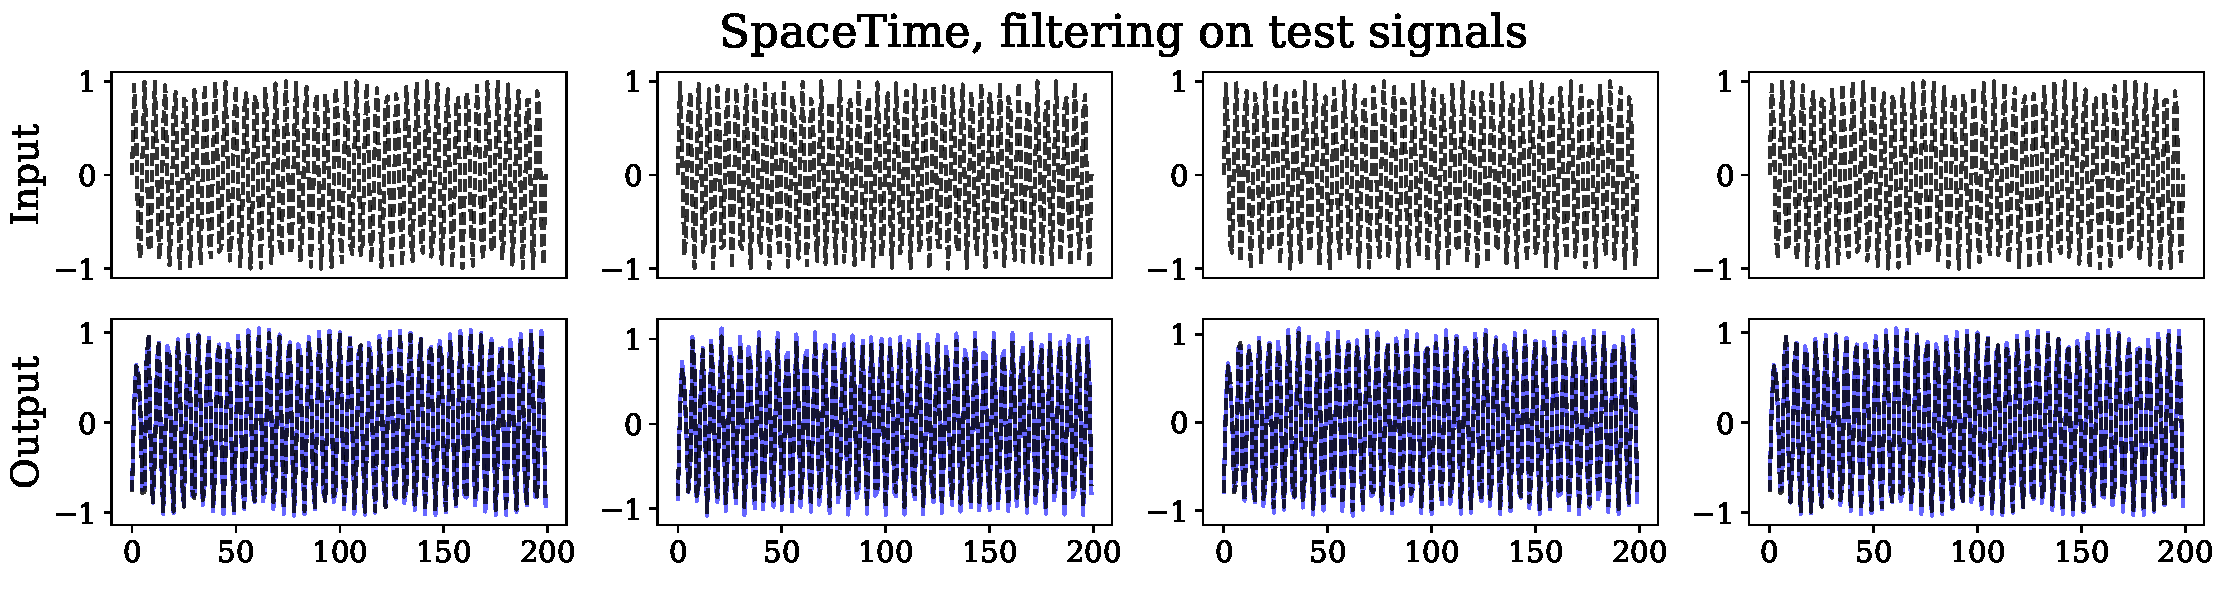
\includegraphics[width=0.99\columnwidth]{_ICLR2023_paper/figures/dsp_SpaceTime.pdf}
%     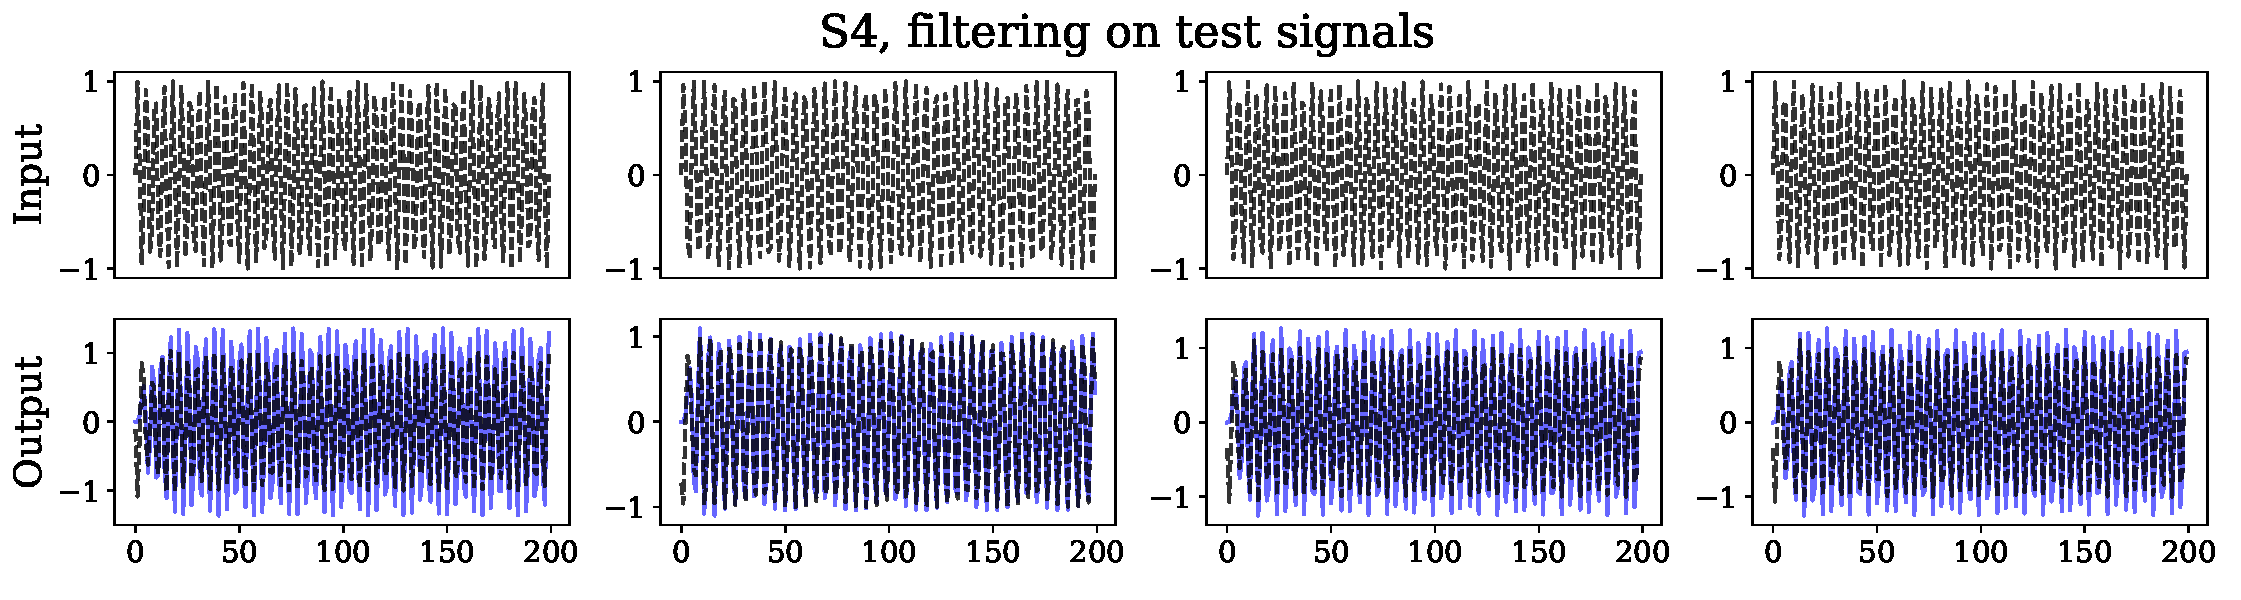
\includegraphics[width=0.99\columnwidth]{_ICLR2023_paper/figures/dsp_S4.pdf}
%     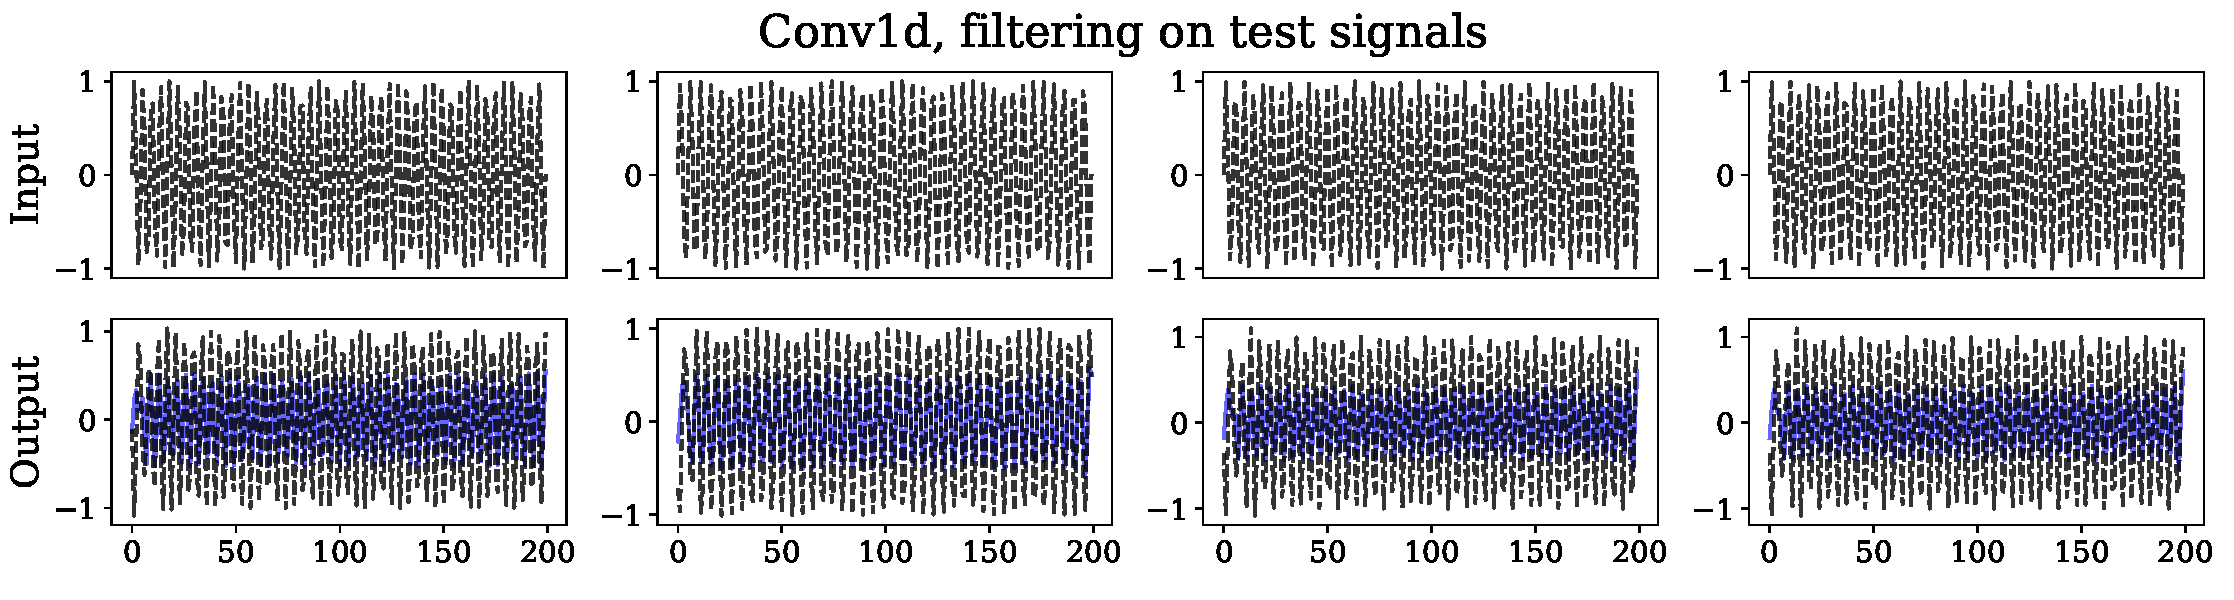
\includegraphics[width=0.99\columnwidth]{_ICLR2023_paper/figures/dsp_Conv1d.pdf}
%     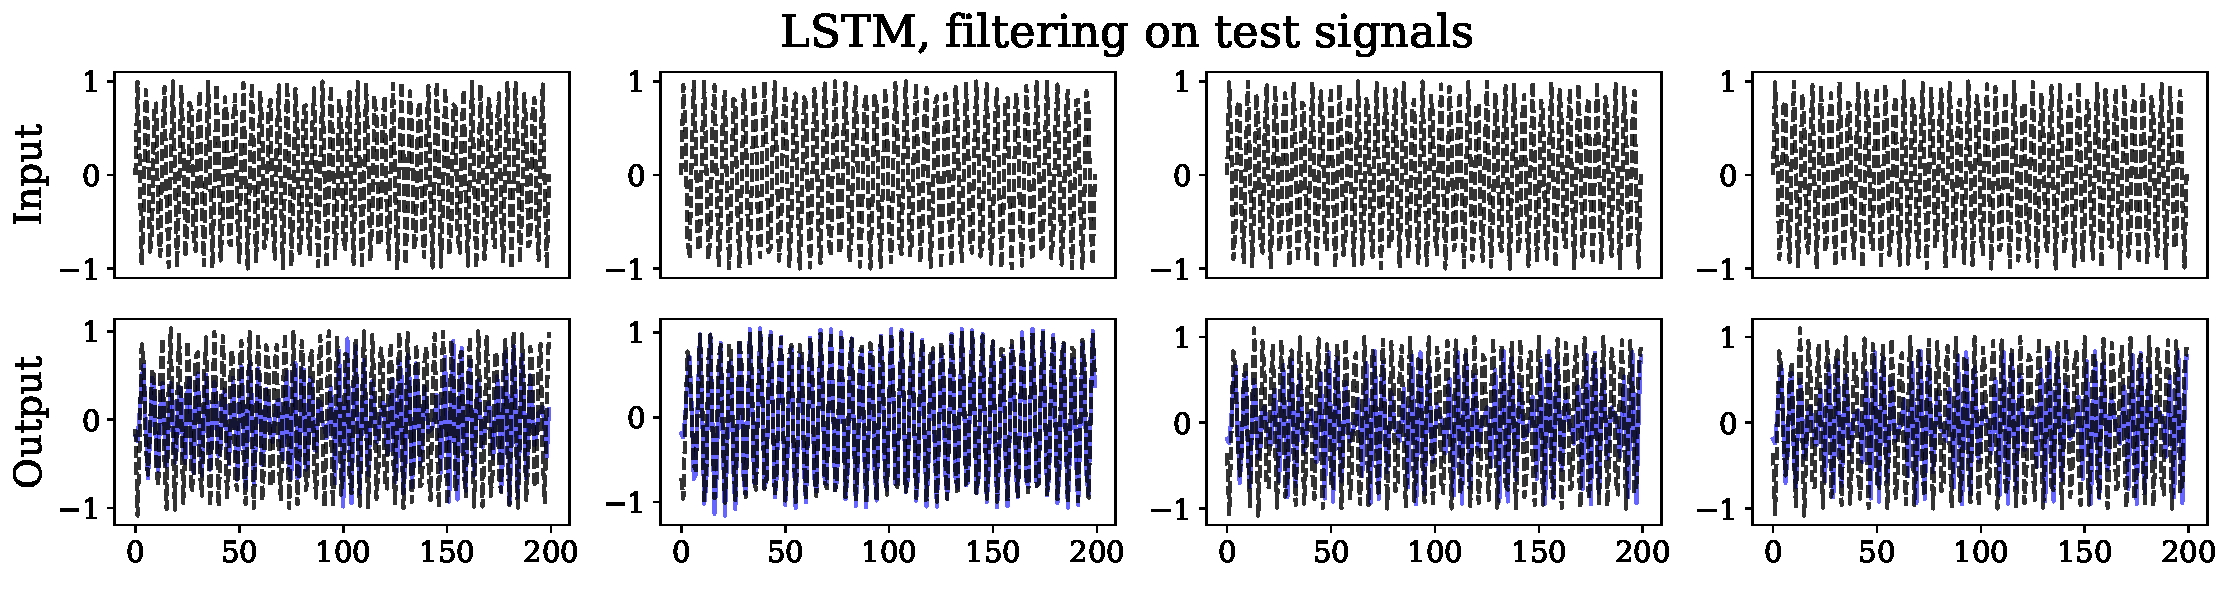
\includegraphics[width=0.99\columnwidth]{_ICLR2023_paper/figures/dsp_LSTM.pdf}
%     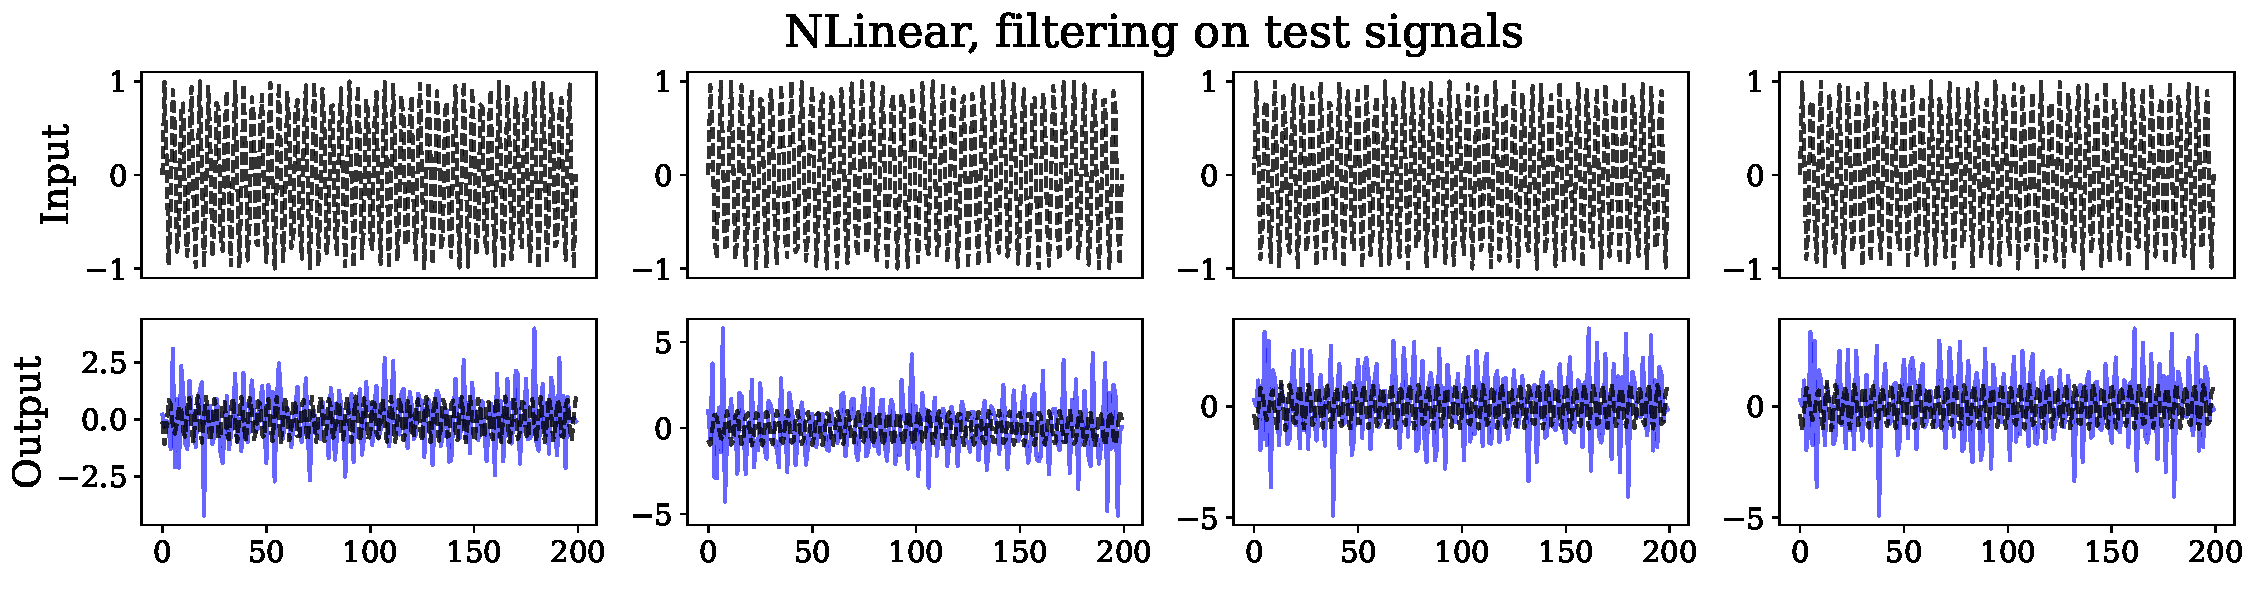
\includegraphics[width=0.99\columnwidth]{_ICLR2023_paper/figures/dsp_NLinear.pdf}
%     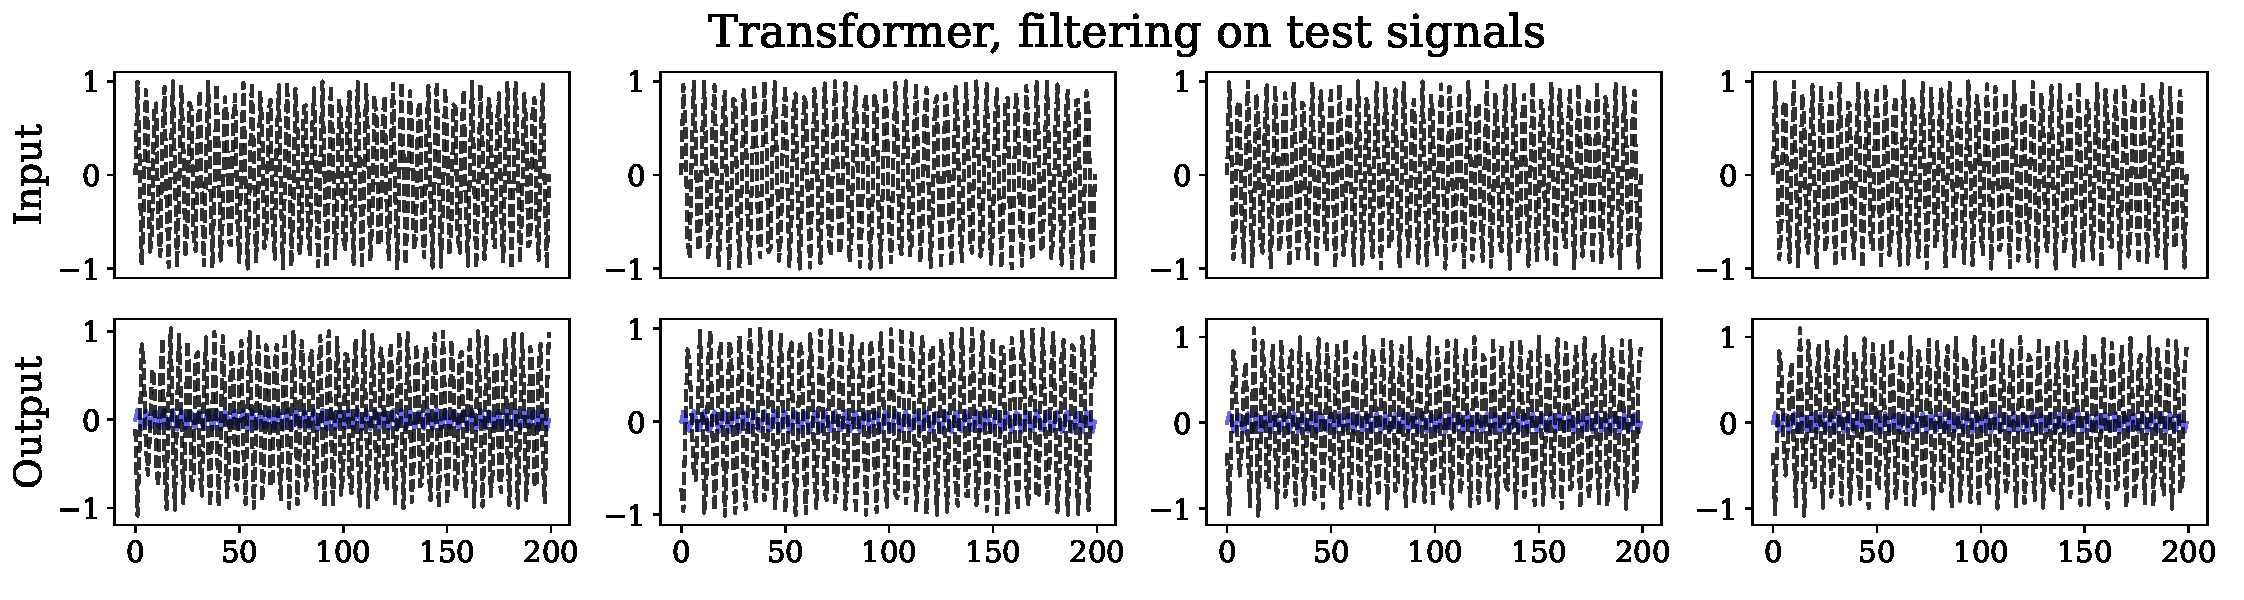
\includegraphics[width=0.99\columnwidth]{_ICLR2023_paper/figures/dsp_Transformer.pdf}
%     \vspace{-2mm}
%     \caption{Testing the capability of different sequence--to--sequence models to approximate the input--output map of digital filters. In blue, we show the output signal filtered by each model. The ground--truth digital filter is a Butterworth of order $10$.}
%     \label{fig:dsp_synthetic}
% \end{figure}
% %


% \begin{sidewaystable}[t]
%     \small
%     \centering
%     \begin{tabular}{c|c|cccccc|ccccc}
%     \toprule
%     %
%     Dataset  & \ourmethod & SES & Theta & TBATS & ETS & (DHR-)ARIMA & PR & CatBoost & DeepAR & N-BEATS & WaveNet & Transformer \\
%     %
%     \midrule
%     M1 Yearly & \underline{135508.3} & 193829.5 & 171458.1 & \textbf{116850.9} & 167739.0 & 175343.8 & 152038.7 & 237644.5 & 173075.1 & 192489.8 & 312821.8 & 182850.6 \\
    
%     M1 Quarterly & \underline{2200.3} & 2545.7&	2282.7	&2673.9&	2408.5&	2538.5&	1909.3&	2161.0& 2313.3&	2267.3&	2271.7&	2231.5  \\    
    
%     M1 Monthly & 2601.1 & 2725.8 & 2564.9 & 2594.5 & 2264.0 & 2450.6 & 2478.8 & 2461.7 & 2202.2 & \textbf{2183.4} & 2578.9 & 3129.8  \\

%     M3 Yearly & 1412.4 & 1172.9&	1106.1&	1386.3	&1189.2	&1662.2	&1181.8&	1341.7&		1157.9&	1117.4&	1147.6&	1084.8 \\
    
%     M3 Quarterly & 676.1 & 670.6&	567.7&	653.6&	598.7&	650.8&	605.5&	698.0&	606.6&	582.8&	606.8&	819.2\\ 
    
%     M3 Monthly & 897.12 & 893.9	&754.0&	765.2	&755.3&	790.8&	830.0&	874.2&	873.7&	796.9&	845.3&	948.4 \\
    
%     M3 Other & 265.56 & 309.7	&242.1&	217.0&	224.1	&220.8	&262.3&	349.9&	277.7&	248.5&	277.0	&271.0 \\
    
%     M4 Quarterly & 718.2 & 732.8&	673.2&	672.7&	674.3&	710.0&	711.9&	714.2&	700.3&	684.7&	697.0&	739.1 \\
    
%     M4 Monthly & 1092.2 & 755.5	&683.7&	743.4&	705.7&	702.1&	720.5&	734.8&	740.3&	705.2&	787.9&	902.4\\ 
    
%     M4 Weekly & \textbf{348.3}& 412.6	&405.2&	356.7&	408.5	&386.3&	350.3&	420.8&	422.2&	330.8&	437.3&	456.9\\ 
    
%     M4 Daily &\textbf{183.2}& 209.8&	210.4&	\underline{208.4}&	230.0	&212.6&	213.0&	263.1	&343.5&	221.7&	220.5&	233.6\\ 
    
%     M4 Hourly & \textbf{255.2} & 1476.8	&1483.7	&469.9&	3830.4&	1563.1&	\underline{313.0} &	344.6&	1095.1&	501.2&	468.1&	391.2\\
    
%     Tourism Yearly & \textbf{74799.2}& 106665.2&	99914.2&	105799.4&	104700.5&	106082.6&	89645.6	&87489.0&	78470.7&	78241.7	&77581.3&	80089.3\\
    
%     Tourism Quarterly & 11608.32& 15000.0&	9254.6&	12001.5	&10812.3	&12564.8	&11746.9	&12788.0	&11762.0&	11306.0	&11546.6	&11724.1 \\
    
%     Tourism Monthly & 3181.2& 7039.4&	2702.0	&3661.5	&2543.0	&3132.4&	2739.4&	3102.8&	2359.9&	2596.2&	2694.2&	2660.1\\
    
%     Pedestrian & 69.6& 228.1&	228.2	&261.3&	278.3&	820.3&	61.8&	60.8&	65.8&	99.3&	68.0&	70.2\\
    
%     Weather & \textbf{2.7}& 2.9	&3.3&	2.9&	3.0&	3.1	&9.1&	3.1&	\textbf{2.7}	&3.1&	3.0	&2.8\\
    
%     NN5 Weekly & \textbf{16.9}& 18.8&	18.7&	18.5&	18.8&	18.6&	18.6&	18.7&	18.5&	17.4&	24.2&	24.0 \\
    
%     Solar $10$ min &7.4& 7.2&	7.2	&10.7&	7.2	&5.6&	7.2	&8.7&	7.2	&6.6&	8.0&	7.2\\
    
%     Solar Weekly &1423.7& 1331.3&	1341.6&	1049.0&	1264.4&	967.9&	1168.2&	1754.2&	873.6&	1307.8&	2569.3&	693.8\\
    
%     Electricity Hourly & \textbf{475.1} & 1026.3&	1026.4&	743.4&	1524.9&	1082.4&	689.9&	582.7&	\underline{478.0} &	510.9&	489.9&	514.7\\
    
%     Electricity Weekly &37802.2& 77067.9&	76935.6&	28039.7	&70369.0&	32594.8&	47802.1&	37289.7	&53100.3&	35576.8	&63916.9&	78894.7\\
    
%     Fred-MD &3743.6& 3103.0&	3898.7&	2295.7&	2341.7	&3312.5&	9736.9&	2679.4&	4638.7&	2813.0&	2779.5&	5098.9\\
    
%     Traffic Hourly &0.03& 0.04&	0.04	&0.05&	0.04	&0.04&	0.03	&0.03&	0.02&	0.02	&0.03&	0.02\\
    
%     Traffic Weekly &\textbf{1.3}& 1.5&	1.5	&1.5&	1.5	&1.5&	1.5&	1.5	&1.5&	1.4	&1.6&	1.9\\
    
%     Hospital &40.1& 26.6&	22.6&	21.3&	22.0	&23.7&	23.5&	23.5&	22.0&	24.2&	23.4&	40.5\\
    
%     Covid &490.1& 403.4&	370.1&	113.0&	102.1&	100.5&	394.1&	607.9&	230.5&	186.5&	1135.4&	480.0\\
    
%     Saugeen & \textbf{24.0} & 39.8	&39.8	&42.6&	50.4&	43.2&	47.7&	\underline{39.3} &	45.3&	48.9&	43.0&	49.1\\
    
%     US Births &630.2& 1369.5&	735.5&	606.5&	607.2&	705.5&	732.1&	618.4&	684.0&	627.7&	768.8&	686.5\\
    
%     Sunspot &3.1& 5.0	&5.0&	3.0	&5.0&	3.0	&4.0&	2.4	&1.1&	14.5&	0.7	&0.5\\
    
%     Car Parts & 0.64 & 0.71&	0.65	&0.71&	0.71&	0.71&	\underline{0.58}&	0.71&	\textbf{0.50}&	1.0&	\underline{0.58}&	0.5\\
    
%     Vehicle Trips &30.4& 36.5&	37.4&	25.7&	37.6&	35.0&	31.7&	27.3&	26.5&	33.6&	29.0&	33.0\\
%     \bottomrule
%     %
%     \end{tabular}
%     \caption{Monash forecasting. We report test RMSE of \ourmethod for each dataset (best result selected via validation RMSE, average of $3$ runs).}
%     \label{tab:monash}
% \end{sidewaystable}


% \begin{table}[t]
%     \small
%     \centering
%     \begin{tabular}{c|cccc}
%     \toprule
%     %
%     Dataset  & Ours & S4S & S4D & S4DPLR  \\
%     %
%     \midrule
%     M1 Yearly & {\color{red!50}$154770.78$} & {\color{red!50}$177978.63$} & $161463.53$ &  \\
%     M1 Quarterly \\
%     M1 Monthly \\
%     M3 Yearly \\
%     M3 Quarterly \\ 
%     M3 Other \\ 
%     M4 Monthly \\ 
%     M4 Weekly \\ 
%     M4 Daily \\ 
%     Tourism Yearly \\
%     Tourism Monthly \\
%     Dominick \\
%     Pedestrian \\
%     Weather
%     NN5 \\
%     Solar $10$ min & $6.72$ &\\
%     Solar Weekly \\
%     Electricity Hourly \\
%     Electricity Weekly \\
%     Fred-MD \\
%     Traffic Hourly \\
%     Traffic Weekly \\
%     Hospital \\
%     Covid \\
%     Saugeen \\
%     US Births \\
%     \bottomrule
%     %
%     \end{tabular}
%     \caption{Monash forecasting. We report average test RMSE of \ourmethod for each dataset ($5$ runs each).}
%     \label{tab:my_label}
% \end{table}


% \begin{sidewaystable}[t]
%     \small
%     \centering
%     \begin{tabular}{c|c|cccccc|ccccc}
%     \toprule
%     %
%     Dataset  & Ours & SES & Theta & TBATS & ETS & (DHR-)ARIMA & PR & CatBoost & FFNN & DeepAR & N-BEATS & WaveNet & Transformer \\
%     %
%     \midrule
%     M1 Yearly & $2$ & $11$ & $6$ & $1$ & $5$ & $8$ & $3$ & $12$ & $4$ & $7$ & $10$ & $13$ & $9$ \\
%     M1 Quarterly \\
%     M1 Monthly \\
%     M3 Yearly \\
%     M3 Quarterly \\ 
%     M3 Other \\ 
%     M4 Monthly \\ 
%     M4 Weekly \\ 
%     M4 Daily \\ 
%     Tourism Yearly \\
%     Tourism Monthly \\
%     Dominick \\
%     Pedestrian \\
%     Weather
%     NN5 \\
%     Solar $10$ min & $6.72$ &\\
%     Solar Weekly \\
%     Electricity Hourly \\
%     Electricity Weekly \\
%     Fred-MD \\
%     Traffic Hourly \\
%     Traffic Weekly \\
%     Hospital \\
%     Covid \\
%     Saugeen \\
%     US Births \\
%     \bottomrule
%     %
%     \end{tabular}
%     \caption{Monash foreacasting. Model rankings (based on test RMSE).}
%     \label{tab:my_label}
% \end{sidewaystable}
\section{Experiment Details}
\label{sec:experiment_details}

\subsection{Model Configurations and Hyperparameters}

We summarize the details required to replicate our experiments below.

\subsubsection{Image Classification}

\textbf{Baseline Model:} For dense models, we use standard implementations of
ViT~\citep{dosovitskiy2020image}, MLP-Mixer{tolstikhin2021mlp} from the
\texttt{timm} library and from the T2T-ViT codebase~\citep{yuan2021tokens}.

The Monarch version of these models simply swap out the dense weight matrices in the attention blocks (projection matrices) and in the FFN block (linear layers) with Monarch matrices.
We set the number of blocks in the block-diagonal matrices to 4.
We also reduce the amount of regularization (stochastic depth) as our Monarch models are smaller than the dense models.

We adopt the hyperparameters (optimizer, learning rate, learning rate
scheduler) from~\citet{yuan2021tokens}.
Details are in~\cref{table:imagenet_hparams}.

We measure the wall-clock training time on V100 GPUs.

\begin{table}[!htbp]
 \caption{Configuration of the ImageNet experiment}   
\centering
\resizebox{0.8\linewidth}{!}{
\noindent\begin{tabular}{@{}c||ccccccc@{}}
  \specialrule{.15em}{.05em}{.05em}
Model&\multicolumn{1}{c}{Optimizer}&\multicolumn{1}{c}{Weight Decay}&\multicolumn{1}{c}{Learning Rate}&\multicolumn{1}{c}{Drop Path}&\multicolumn{1}{c}{Warmup/Epoch}\\
  \specialrule{.15em}{.05em}{.05em}
ViT-Small& AdamW & 0.05 & 0.001 & 0.1& 5/300 \\
Monarch-ViT-Small& AdamW & 0.05 & 0.001 &0& 5/300 \\
ViT-Base& AdamW & 0.05 & 0.001 &0.1& 5/300 \\
Monarch-ViT-Base& AdamW & 0.05 & 0.001 &0& 5/300 \\
  \specialrule{.15em}{.05em}{.05em}
Mixer-Small &AdamW& 0.1 &0.001&0.1& 5/300 \\
Monarch-Mixer-Small &AdamW&0.1 &0.001& 0 & 5/300 \\
Mixer-Base &AdamW& 0.1 &0.001&0.1& 5/300 \\
Monarch-Mixer-Base &AdamW &0.1 &0.001& 0 & 5/300 \\
  \specialrule{.15em}{.05em}{.05em}
\end{tabular}
}
\label{table:imagenet_hparams}
\end{table}

We follow the naming convention in the Vision Transformer paper and MLP-Mixer paper. In particular, ViT-S and ViT-B refers to the small and base ViT models respectively, and 16 refers to the patch size of 16x16. The MLP-Mixer models follow the same convention.

\subsubsection{Language Modeling}
For dense models, we use standard implementations of
GPT-2~\citep{radford2019language} from Huggingface \texttt{transformers} library and from Nvidia's Megatron-LM repo. 
We follow the training recipe of the Megatron-LM repo.

The Monarch version of these models simply swap out the dense weight matrices in the attention blocks (projection matrices) and in the FFN block (linear layers) with Monarch matrices.
We set the number of blocks in the block-diagonal matrices to 4.
We also reduce the regularization strength (dropout) as our model is smaller.

We report the hyperparameters used in~\cref{table:wt103} and~\cref{table:owt}.
We use an effective batch size of 512, and use gradient accumulation to fit into available GPU memory.

We measure the wall-clock training time on V100 GPUs.
\begin{table}[!h]
    \vspace{-0.5cm}
\centering
\caption{Configuration of the WikiText-103 experiments}
\resizebox{0.8\linewidth}{!}{
\noindent\begin{tabular}{@{}c||ccccccc@{}}
  \specialrule{.15em}{.05em}{.05em}
Model&\multicolumn{1}{c}{Optimizer}&\multicolumn{1}{c}{Weight Decay}&\multicolumn{1}{c}{Learning Rate}&\multicolumn{1}{c}{Dropout}&\multicolumn{1}{c}{Warmup/Epoch}\\
  \specialrule{.15em}{.05em}{.05em}
GPT-2-small& AdamW & 0.1 & 6e-4 & 0.1& 10/100 \\
Monarch-GPT-2-small& AdamW & 0.1 & 6e-4 & 0.0 & 10/100 \\
GPT-2-medium& AdamW & 0.1 & 1.5e-4 & 0.1& 10/100 \\
Monarch-GPT-2-medium & AdamW & 0.1 & 1.5e-4 & 0.0 & 10/100 \\
  \specialrule{.15em}{.05em}{.05em}
\end{tabular}
}
\label{table:wt103}
\end{table}

\begin{table}[!h]
\vspace{-0.5cm}
\centering
\caption{Configuration of the OpenWebText experiments}
\resizebox{0.8\linewidth}{!}{
\noindent\begin{tabular}{@{}c||ccccccc@{}}
  \specialrule{.15em}{.05em}{.05em}
Model&\multicolumn{1}{c}{Optimizer}&\multicolumn{1}{c}{Weight Decay}&\multicolumn{1}{c}{Learning Rate}&\multicolumn{1}{c}{Dropout}&\multicolumn{1}{c}{Warmup/Total iterations}\\
  \specialrule{.15em}{.05em}{.05em}
GPT-2-Small& AdamW & 0.1 & 6e-4 & 0.1& 4k/400k \\
Monarch-GPT-2-Small & AdamW & 0.1 & 6e-4 & 0.0 & 4k/400k \\
GPT-2-Medium& AdamW & 0.1 & 1.5e-4 & 0.1& 4k/400k \\
Monarch-GPT-2-Medium & AdamW & 0.1 & 1.5e-4 & 0.0 & 4k/400k \\
  \specialrule{.15em}{.05em}{.05em}
\end{tabular}
}
\label{table:owt}
\end{table}


\subsection{Details for PDE Solving}
We adopt the experiment setting and data generation of Navier-Stokes Equation from FNO~\citep{li2020fourier}. It considers the 2-d Navier-Stokes equation for a viscous, incompressible fliud in vorticity form on the unit tortus:
\begin{align}
    \partial_{t} w(x, t) + u(x, t) \cdot \nabla w(x, t) & = v \Delta w(x, t) + f(x), & x \in (0, 1)^2, t \in (0, T] \\
    \nabla w(x, t) & = 0, & x \in (0, 1)^2, t \in (0, T] \\
    w(x, 0) & = w_0(x), & x \in (0, 1)^2 \\
\end{align}
where $u \in C([, T0])$;$H_{per}((0, 1)^2; \mathbb{R}^2))$ for any $r>0$ is the velocity field, $w=\nabla \times u$ is the vorticity, $w_0 \in L^2_{per}((0, 1)^2; \mathbb{R})$ is the initial vorticity, $v \in \mathbb{R_{+}}$ is the viscosity coefficient, and $f \in L_{per}^2((0, 1)^2; \mathbb{R})$ is the forcing function. 
$T$ represents the time interval since it is time-dependent equation. $v$ represents the viscosity. N represents the number of training pairs or data. \cref{table:pde} shows the results for viscosities $v=1e-3, 1e-4, 1e-5$, $T=50, 30, 20$ respectively and use $N=1000$. 

\subsection{Details for GPT-2 Downstream Tasks}
We train Pixelfly-GPT2-small on a larger scale dataset, OpenWebText, and evaluate the downstream quality on zero-shot generation and classification tasks from~\citep{zhao2021calibrate}, achieving comparable and even better performance to the dense model. Specifically, the datasets contains five popular classification tasks: SST2, Trec, CB, Agnews, and Dbpedia. We also adapated the calibrated metric from~\citep{zhao2021calibrate} for evaluation. Results for each individual task are shown in~\cref{table:gpt_finetune_full}. 

\begin{table}[h]
  \small
  \centering
  \vspace{-3mm}
  \caption{\label{table:gpt_finetune_full}The performance (accuracy) of GPT-2-medium trained with Monarch reverse sparsification and with conventional dense training on text classification benchmarks.}
  \setlength{\tabcolsep}{5pt}
  \vspace{1em}
   \resizebox{0.7\linewidth}{!}{
  \begin{tabular}{@{}c||ccccc@{}}
    \specialrule{.15em}{.05em}{.05em}
    Model&\multicolumn{1}{c}{OpenWebText (ppl)}&\multicolumn{1}{c}{Speedup}& \multicolumn{1}{c}{Classification (avg acc)} \\
    \specialrule{.15em}{.05em}{.05em}
    GPT-2m& 68.3 & 37.0 & 10.7 & 52.0 & 26.6\\
    Monarch-GPT-2m& 72 & 38.6 & 12.5 & 47.3 & 23.0 \\
    \specialrule{.15em}{.05em}{.05em}
  \end{tabular}
  }
  \vspace{-3mm}
\end{table}

\subsection{Details for BERT Pretraining}
\label{subsec:bert_details}

We follow the training procedure and hyperparameters of the reference
implementation from Nvidia Deep Learning examples
(\url{https://github.com/NVIDIA/DeepLearningExamples}).
In particular, we use the LAMB optimizer with learning rate 4e-3.
We use as large a minibatch size as possible that still fits in the GPU memory
(A100-40GB), and use gradient accumulation to reach an effective batch size of
64k sequences for phase 1 (maximum sequence length 128) and 32k for phase 2
(maximum sequence legnth 512).
We train is mixed precision (fp16 and fp32).

We use all the optimizations that were in Nvidia's BERT implementation
in MLPerf 1.1:
\begin{enumerate}
  \item Only compute the prediction scores (last layer) for masked tokens as
  the outputs of other tokens are not used to compute the masked language
  modeling loss.
  \item Remove padding tokens and only compute the attention for non-padding
  tokens.
  \item Use a fused CUDA kernel (FMHA) that combines 4 steps into one kernel: computes
  $Q K^T$, take softmax, apply dropout, multiply by $V$, where $Q, K, V$ are the
  query, key, and value respectively.
  \item Fuse matrix multiplication and adding bias into one CUDA kernel in the feed-forward network
  (FFN) layers. The gradient of the bias is also fused with the matrix
  multiplication the backward pass.
  \item Fuse matrix multiplication and adding bias into one CUDA kernel in the
  attention output projection.
  \item Fuse dropout and adding residual in the residual connection at the end
  on the attention and FFN blocks.
\end{enumerate}

We train with DeepSpeed~\citep{rasley2020deepspeed} ZeRO optimizer stage 1 to
shard the optimizer states, thus reducing GPU memory usage and allowing us to
use larger batch sizes.
For the Nvidia MLPerf implementation, we report the speed for both Apex's
automatic mix-precision (AMP) level O2 (as in the original implementation), and
DeepSpeed ZeRO optimizer.

\subsection{Accelerated Multi-coil MRI Reconstruction}
\label{sec:experiment_details_mri}

\subsubsection{Background}
In multi-coil MRI, multiple receiver coils (i.e. sensors) acquire complex-valued measurements in the spatial frequency (a.k.a. \textit{k-space}) domain. These measurements are modulated by the spatially-varying sensitivity maps, which characterize the sensitivity of each coil to the imaging target. In accelerated MRI, scan times are reduced by decreasing the number of samples acquired in k-space. Because the data is sampled below the Nyquist rate, reconstructing the underlying image is an ill-posed problem.

The forward problem for accelerated multi-coil MRI can be written as the matrix equation
\begin{equation*}
    y = \Omega\boldsymbol{F}\boldsymbol{S}x + \epsilon
\end{equation*}
where $\Omega$ is the binary undersampling mask that indexes acquired samples in k-space, $y$ is the vectorized measured signal in k-space, $\boldsymbol{F}$ is the discrete Fourier transform matrix, $\boldsymbol{S}$ is the receiver coil sensitivity maps,  $x$ is the ground-truth signal in image-space, and $\epsilon$ is additive complex Gaussian noise. The acceleration factor is given by $R = \frac{\sum_i^{|N|} \Omega_i}{|\Omega|}$.

\subsubsection{Experimental Details}

\paragraph{Dataset.} We benchmark our method on the SKM-TEA Raw Data Track, which consists of dual-echo 3D MRI scans \citep{desai2021skm}. Scans are accelerated using Poisson Disc undersampling masks distributed with the dataset. During training, Poisson Disc masks are generated, cached, and applied to mask the k-space data to simulate accelerated scans.

\paragraph{Matrix Shape.} Like all matrices, Monarch matrices have an explicit shape constraint, which is a limitation of these matrices for MRI reconstruction tasks. Thus, the SKM-TEA dataset was filtered to include scans of shape $512 \times 512 \times 160$, which is the most frequently occuring scan shape. A total of 3 scans were dropped from the original 155 scans in the dataset. Our method and all baselines were trained on this filtered dataset.

\begin{table}[!ht]
    \vspace{-0.5cm}
\centering
\caption{Baseline configurations of the SKM-TEA MRI reconstruction experiments.}
\resizebox{0.6\linewidth}{!}{
\noindent\begin{tabular}{c||cccccc}
  \specialrule{.15em}{.05em}{.05em}
Model & Params & Optimizer & Weight Decay & Learning Rate & Epoch \\
  \specialrule{.15em}{.05em}{.05em}
SENSE & --- & --- & --- & --- & --- \\
U-Net &  7.8M & Adam & 1e-4 & 1e-3 & 20 \\
mSENSE  & 57.5K & Adam & 1e-4 & 1e-3 & 20 \\
  \specialrule{.15em}{.05em}{.05em}
\end{tabular}
}
\label{table:skmtea-config}
\end{table}


\paragraph{Baselines.} We compare our method to two baselines, SENSE and U-Net. Parameter count and hyperparameters are available in Table \ref{table:skmtea-config}.
\begin{itemize}
    \item \textit{SENSE}: SENSE performs a linear combination of the images acquired on each coil \citep{pruessmann1999sense}. Here, the inverse fsat Fourier transform (IFFT) is applied to the acquired k-space for each coil. The resulting images are combined into a single complex image by weighting each coil image by corresponding coil sensitivity maps. In accelerated MRI, the unsampled frequencies are zero-valued; thus, SENSE produces a \textit{zero-filled image}. Note, SENSE does not require any training.
    \item \textit{U-Net}: U-Net is a popular fully convolutional neural network baseline for MRI reconstruction \citep{ronneberger2015u}. We use the default implementation and hyperparameters used by \citet{desai2021skm} to benchmark the SKM-TEA dataset. In this approach, the SENSE-reconstructed zero-filled image is mapped to SENSE-reconstructed ground truth images.
\end{itemize}

\paragraph{Monarch-SENSE (mSENSE):} We propose a modification to the SENSE method, in which the (IFFT) is parameterized by a factorized Monarch matrix. This matrix is initialized to the IFFT but, unlike SENSE, is learnable. While mSENSE is trainable, it has 137x fewer trainable parameters than U-Net.

\paragraph{Metrics:} We evaluate reconstruction performance using peak signal-to-noise ratio (pSNR) and structural similarity (SSIM) on both echoes (echo1 - E1, echo2 - E2) separately. Both metrics were computed on the 3D volume of each echo.

\paragraph{Extended Results.} We provide sample reconstructions of SENSE, mSENSE, and U-Net in data-limited settings for first (Fig.~\ref{fig:mri-data-limited-echo1}) and second (Fig.~\ref{fig:mri-data-limited-echo2}) echoes. Both SENSE and U-Net reconstructed images have aliasing artifacts. Due to the random Poisson Disc undersampling pattern, these artifacts are incoherent, causing them to manifest as blurring around fine structures and edges. In contrast, mSENSE can recover these structures with higher fidelity. Even in the second echo, which has lower signal-to-noise ratio (SNR) than the first echo, mSENSE does not overblur the image.

\begin{figure}
    \centering
    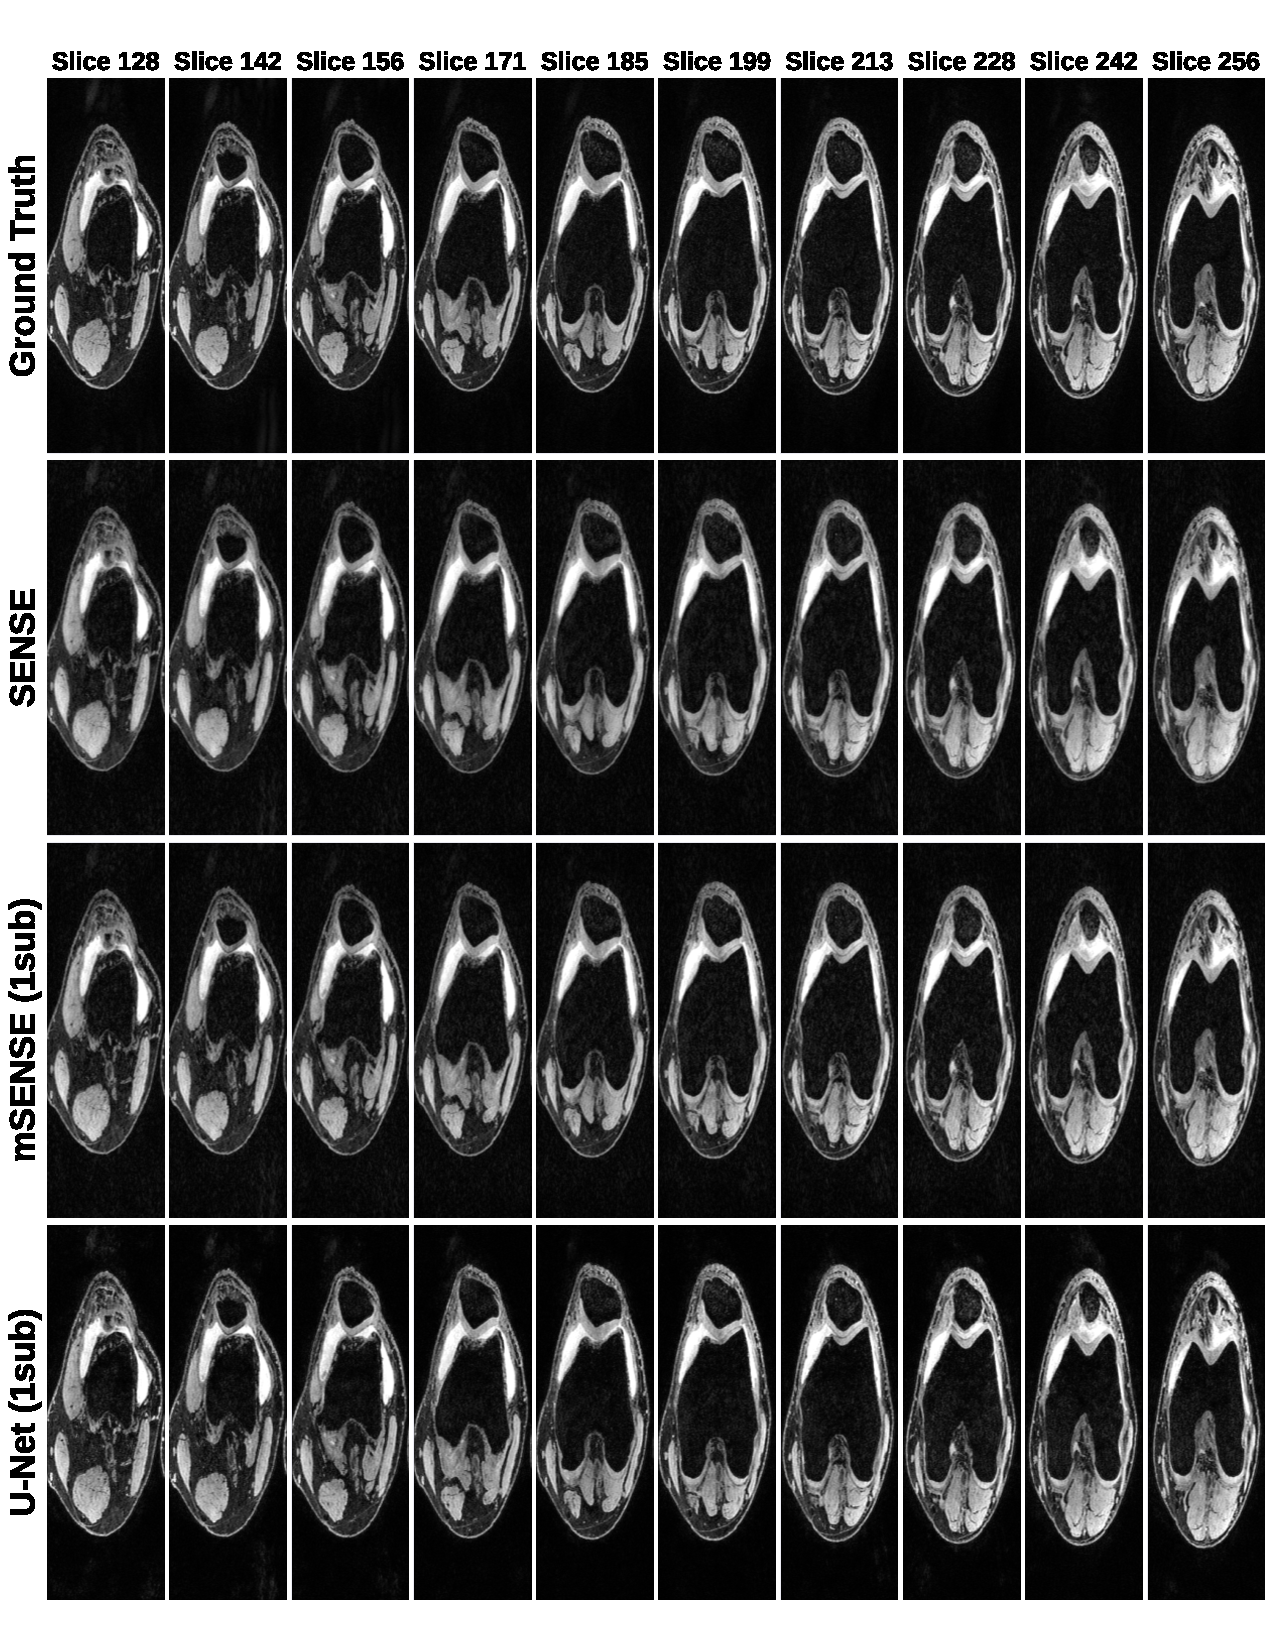
\includegraphics[width=0.9\linewidth]{figures/sample-mri-echo1.pdf}
    \vspace{-1em}
    \caption{Sample reconstructions at 2x acceleration for the first echo in the SKM-TEA dataset using SENSE, Monarch-SENSE (mSENSE), and U-Net. Both mSENSE and U-Net are trained with 1 training scan. SENSE is an untrained method.}
    \label{fig:mri-data-limited-echo1}
\end{figure}

\begin{figure}
    \centering
    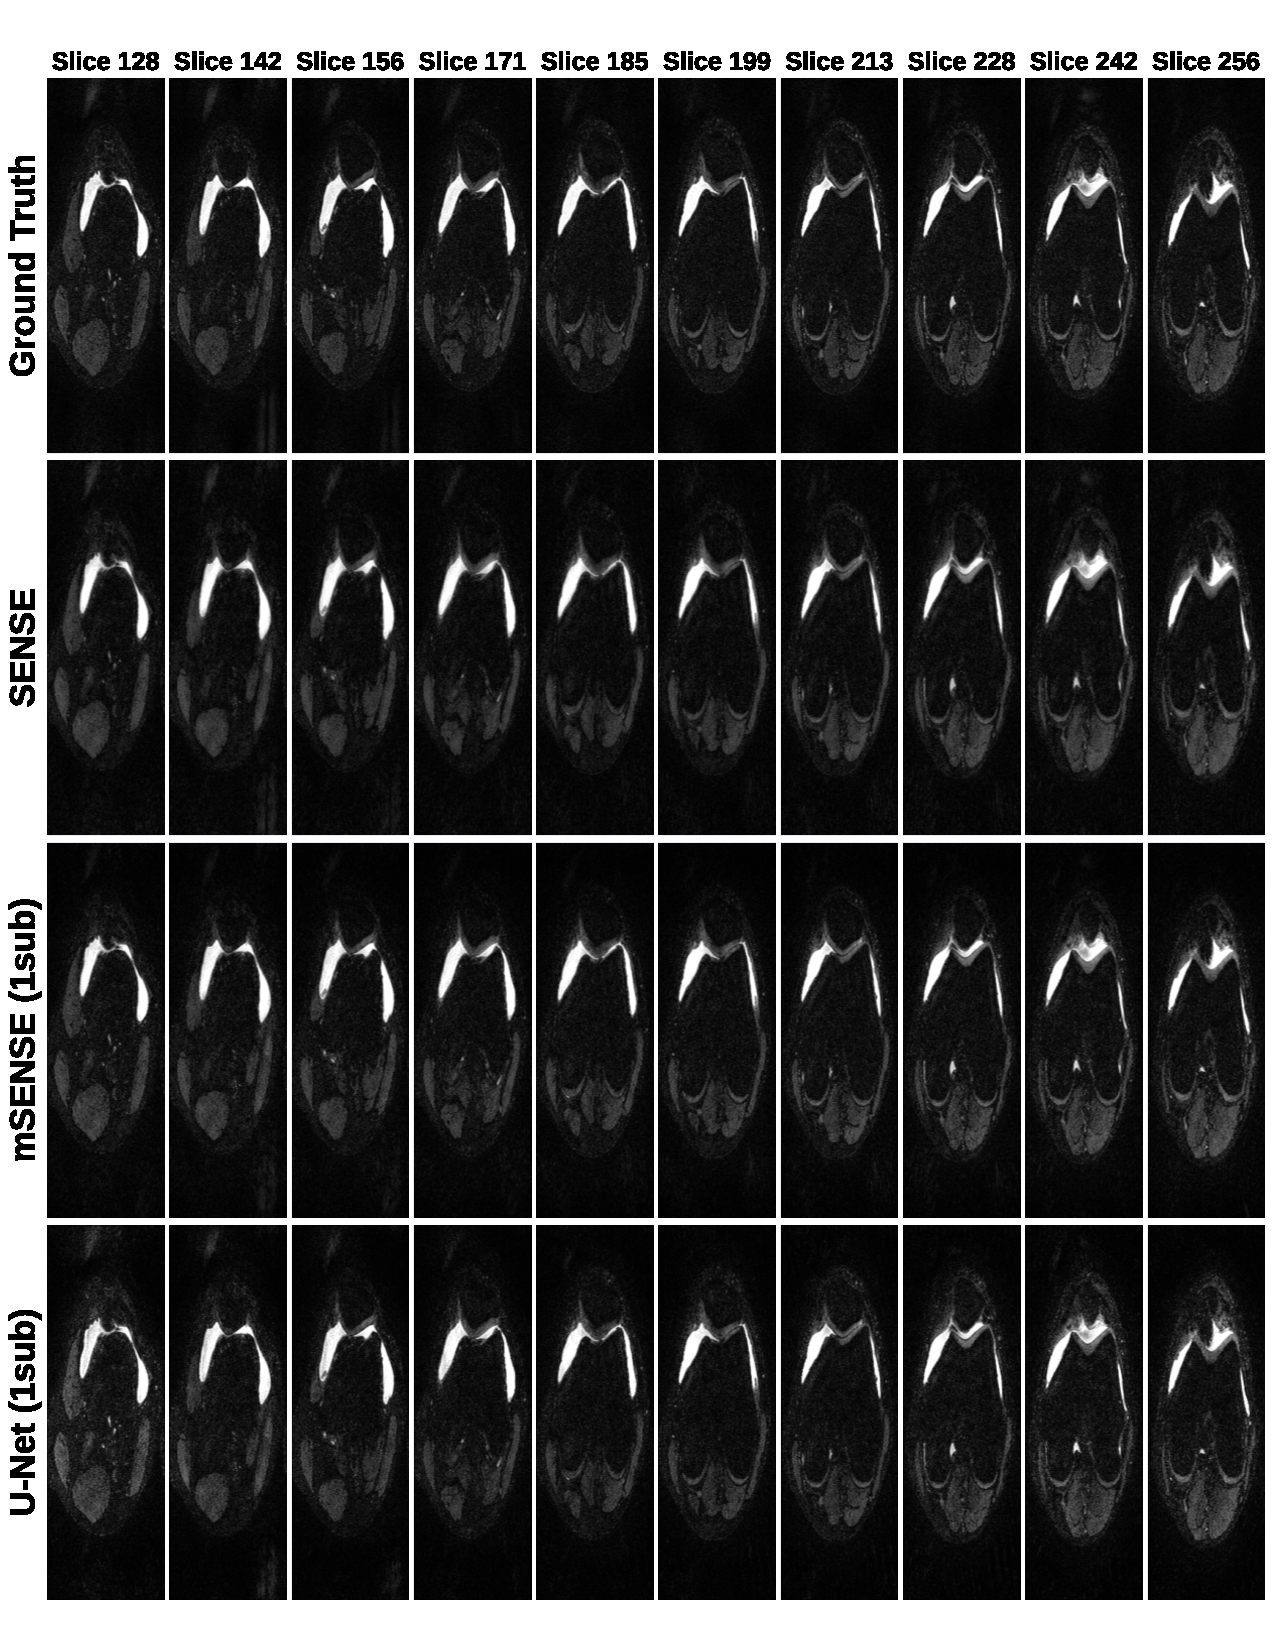
\includegraphics[width=6in]{figures/sample-mri-echo2.pdf}
    \vspace{-1em}
    \caption{Sample reconstructions at 2x acceleration for the second echo in the SKM-TEA dataset using SENSE, Monarch SENSE (mSENSE), and U-Net. Both mSENSE and U-Net are trained with 1 training scan. SENSE is an untrained method.}
    \label{fig:mri-data-limited-echo2}
\end{figure}







\section{Extended experimental results} \label{app:exp_results}

\subsection{Expressivity on digital filters}

% {\ourmethod{} can approximate the frequency response of digital filters}

We experimentally verify whether \ourmethod{} can approximate the input--output map of digital filter admitting a state--space representation, with improved generalization over baseline models given test inputs of unseen frequencies.

We generate a dataset of $1028$ sinusoidal signals of length $200$
\[
x(t) = \sin{(2\pi \omega t})
\]
where $\omega \in [2, 40]~\bigcup~[50, 100]$ in the training set and $\omega \in (40, 50)$ in the test set. The outputs are obtained by filtering $x$, i.e., $y = \mathcal{F}(x)$  where $\mathcal{F}$ is in the family of digital filters. 

We introduce common various sequence-to-sequence layers or models as baselines: the original S4 diagonal plus low--rank \citep{gu2021efficiently}, a single-layer LSTM, a single 1d convolution (Conv1d), a dense linear layer (NLinear), a single self--attention layer. All models are trained for $800$ epochs with batch size $256$, learning rate $10^{-3}$ and Adam. We repeat this experiment for digital filters of different orders \citep{oppenheim1999discrete}. The results are shown in Figure \ref{fig:dsp_synthetic}. \ourmethod{} learns to match the frequency response of the target filter, producing the correct output for inputs at test frequencies. 


\begin{table}[h]
\caption{Comparing sequence models on the task of approximating the input--output map defined by digital filters of different orders. Test RMSE on held-out inputs at unseen frequencies.}
    \label{tab:my_label}
    \centering
    \begin{tabular}{cc|ccccccc}
    \toprule
    %
    Filter & Order & \ourmethod & S4 & Conv1D & LSTM & NLinear & Transformer \\
    %
    \midrule
    Butterworth & $2$ & $0.0055$ & $0.0118$ & $0.0112$ & $0.0115$ & $1.8420$ & $0.5535$ \\
    & $3$ & $0.0057$ & $0.3499$ & $0.0449$ & $0.0231$ & $1.7085$ & $0.6639$ \\
    & $10$ & $0.0039$ & $0.8077$ & $0.4747$ & $0.2753$  & $1.5162$ & $0.7191$ \\
    \midrule
    Chebyshev $1$ & $2$ & $0.0187$ & $0.0480$ & $0.0558$ & $0.0285$ & $1.9313$ & $0.2452$ \\
    & $3$ & $0.0055$ & $0.0467$ & $0.0615$ & $0.0178$ & $1.8077$ & $0.4028$ \\
    & $10$ & $0.0620$ & $0.6670$ & $0.1961$ & $0.1463$ & $1.5069$ & $0.7925$ \\
    \midrule
    Chebyshev $2$ & $2$ & $0.0112$ & $0.0121$ & $0.0067$ & $0.0019$ & $0.4101$ & $0.0030$ \\
    & $3$ & $0.0201$ & $0.0110$ & $0.0771$ & $0.0102$ & $0.4261$ & $0.0088$\\
    & $10$ & $0.0063$ &  $0.6209$ & $0.3361$ & $0.1911$ & $1.5584$ & $0.7936$\\
    \midrule
    Elliptic & $2$ & $0.0001$ & $0.0300$ & $0.0565$ & $0.0236$ & $1.9150$ & $0.2445$ \\
    & $3$ & $0.0671$ & $0.0868$ & $0.0551$ & $0.0171$ & $1.8782$  & $0.4198$ \\
    & $10$ & $0.0622$ & $0.0909$ & $0.1352$ & $0.1344$ & $1.4901$ & $0.7368$ \\
    %
    \bottomrule
    %
    \end{tabular}
    
\end{table}
%
% \begin{figure}[h]
%     \centering
%     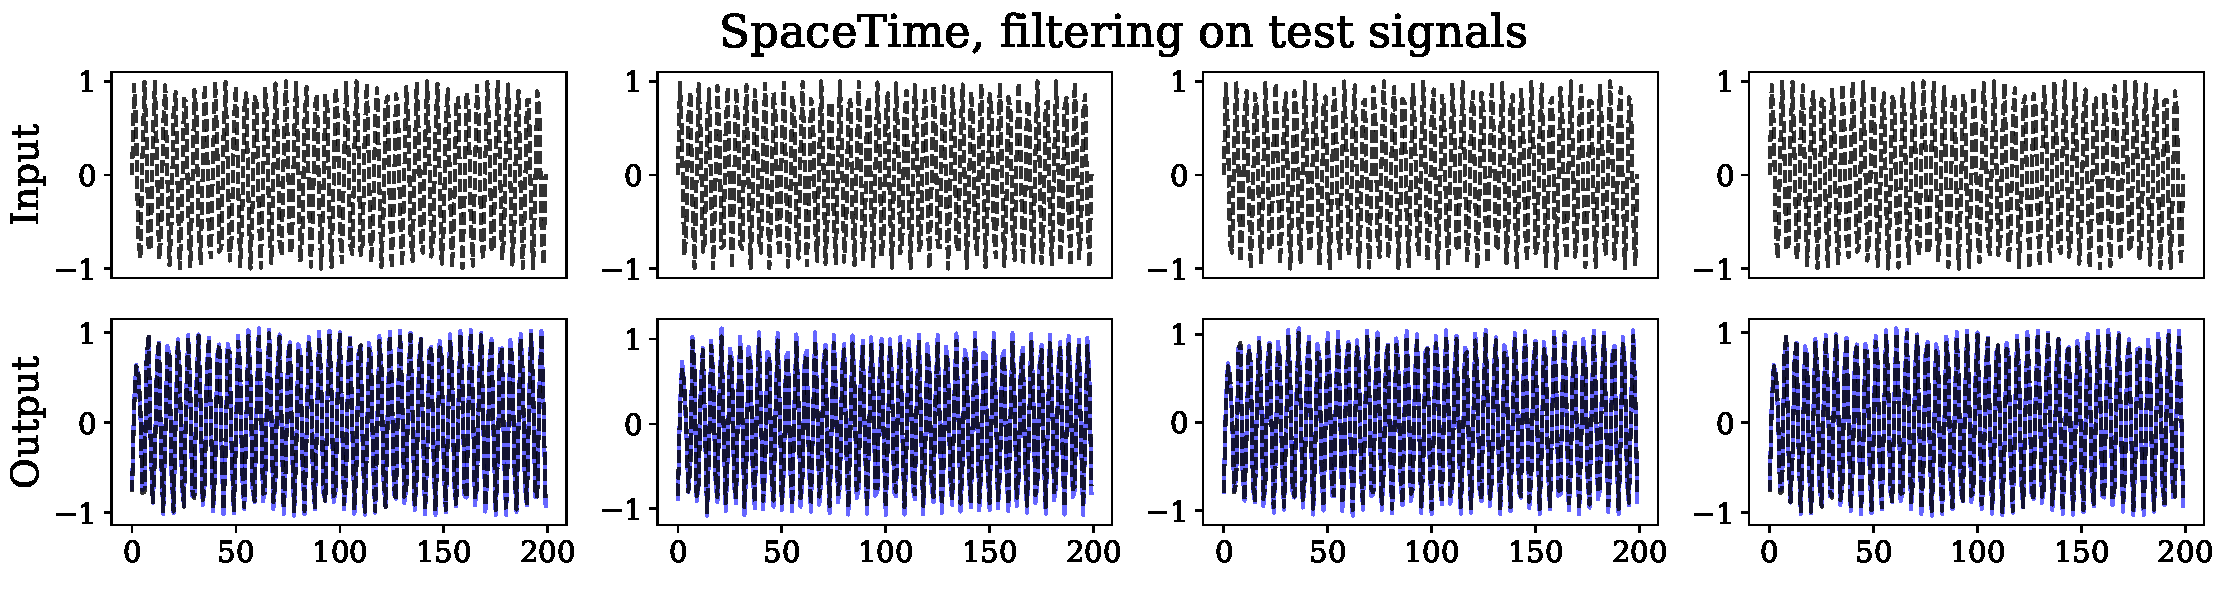
\includegraphics[width=0.99\columnwidth]{_ICLR2023_paper/figures/dsp_SpaceTime.pdf}
%     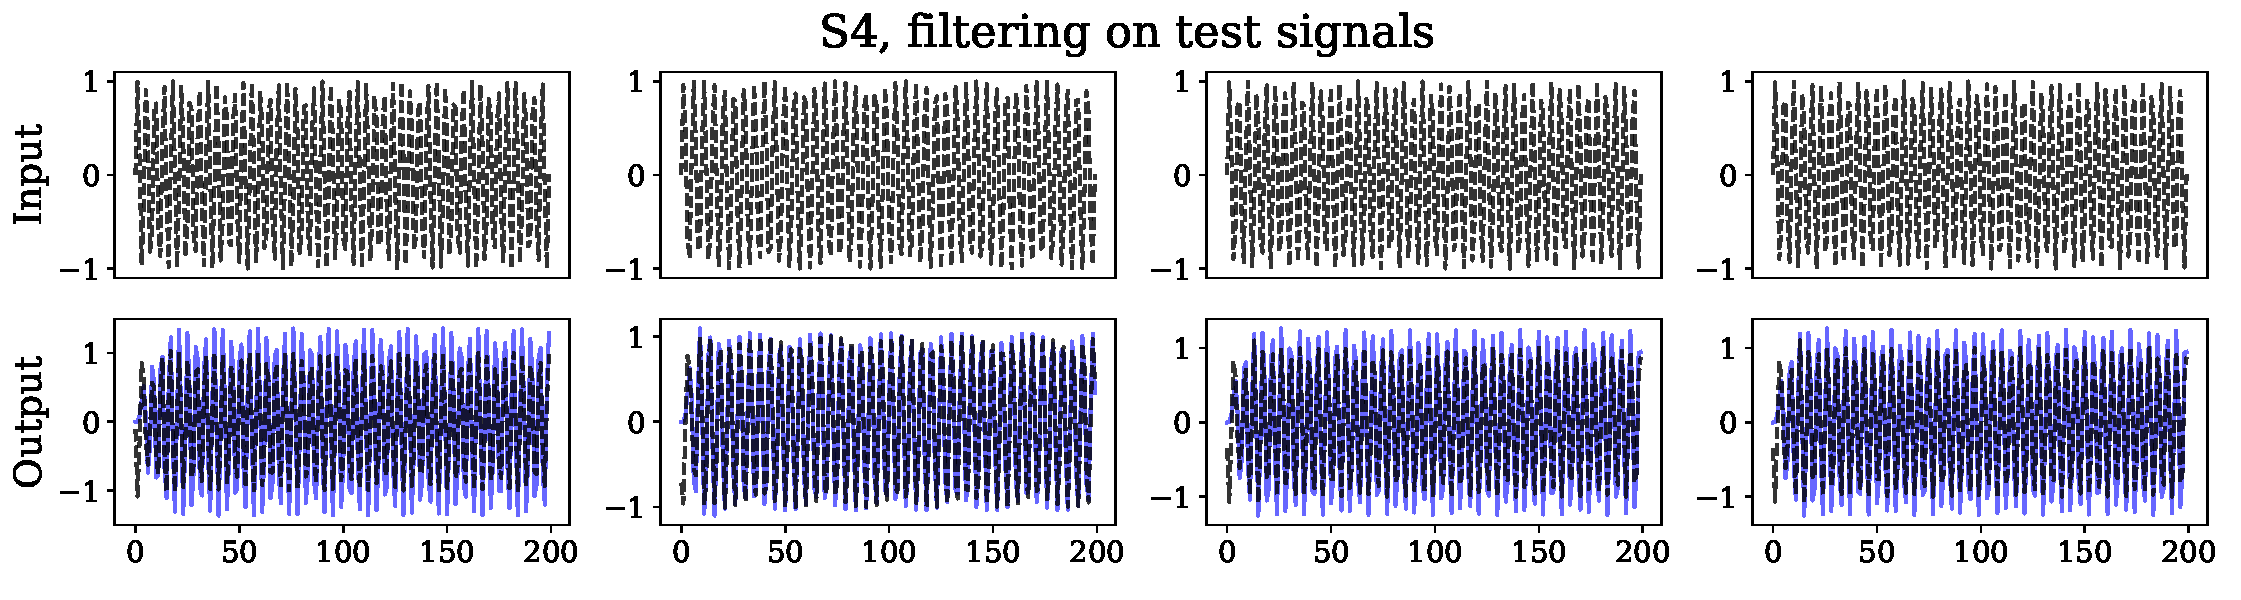
\includegraphics[width=0.99\columnwidth]{_ICLR2023_paper/figures/dsp_S4.pdf}
%     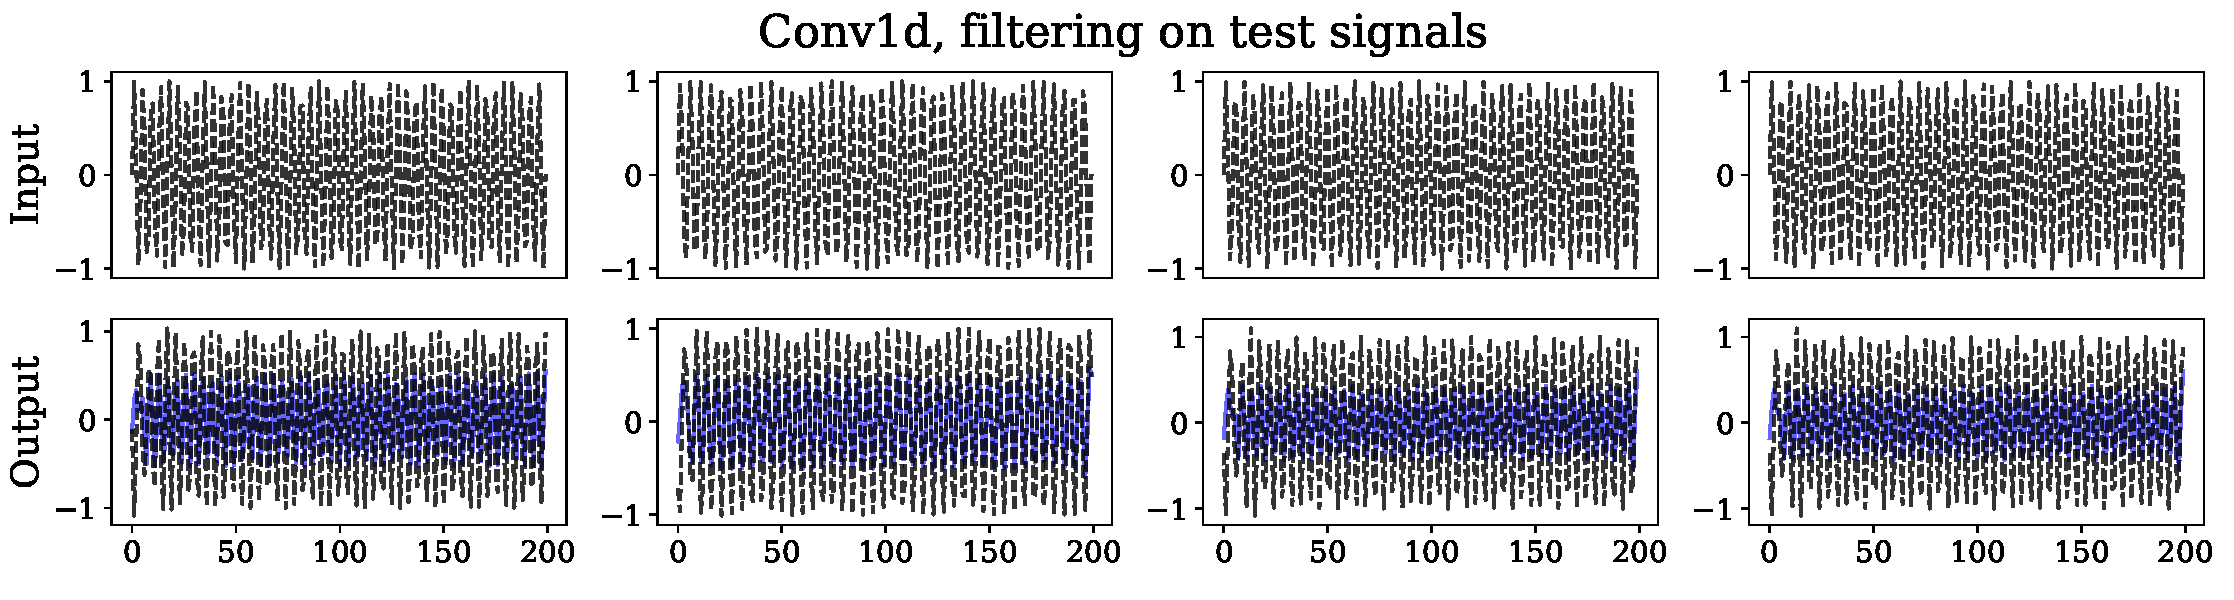
\includegraphics[width=0.99\columnwidth]{_ICLR2023_paper/figures/dsp_Conv1d.pdf}
%     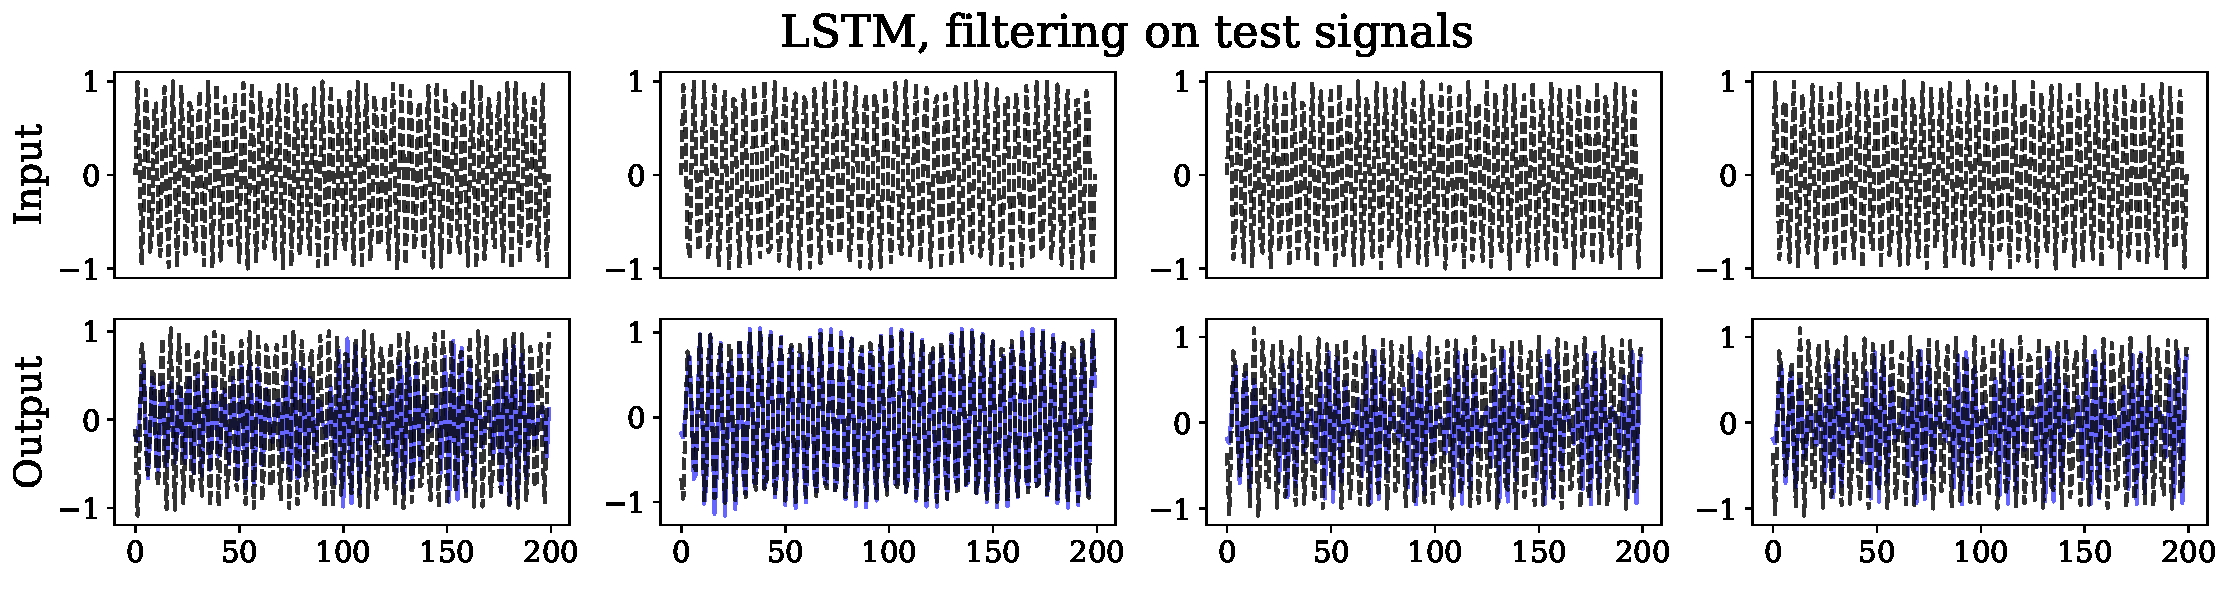
\includegraphics[width=0.99\columnwidth]{_ICLR2023_paper/figures/dsp_LSTM.pdf}
%     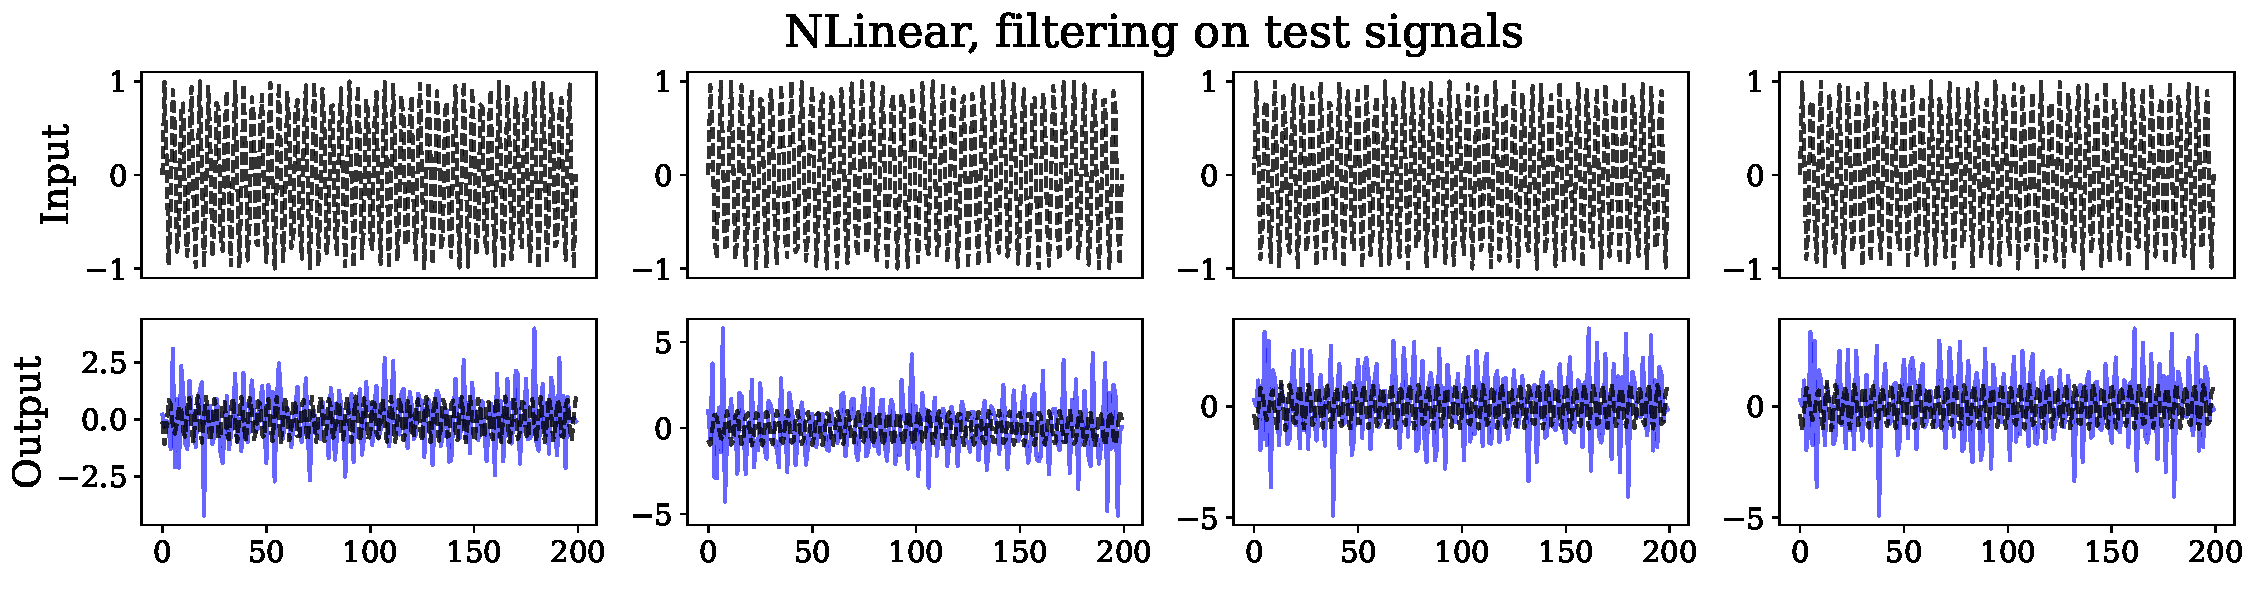
\includegraphics[width=0.99\columnwidth]{_ICLR2023_paper/figures/dsp_NLinear.pdf}
%     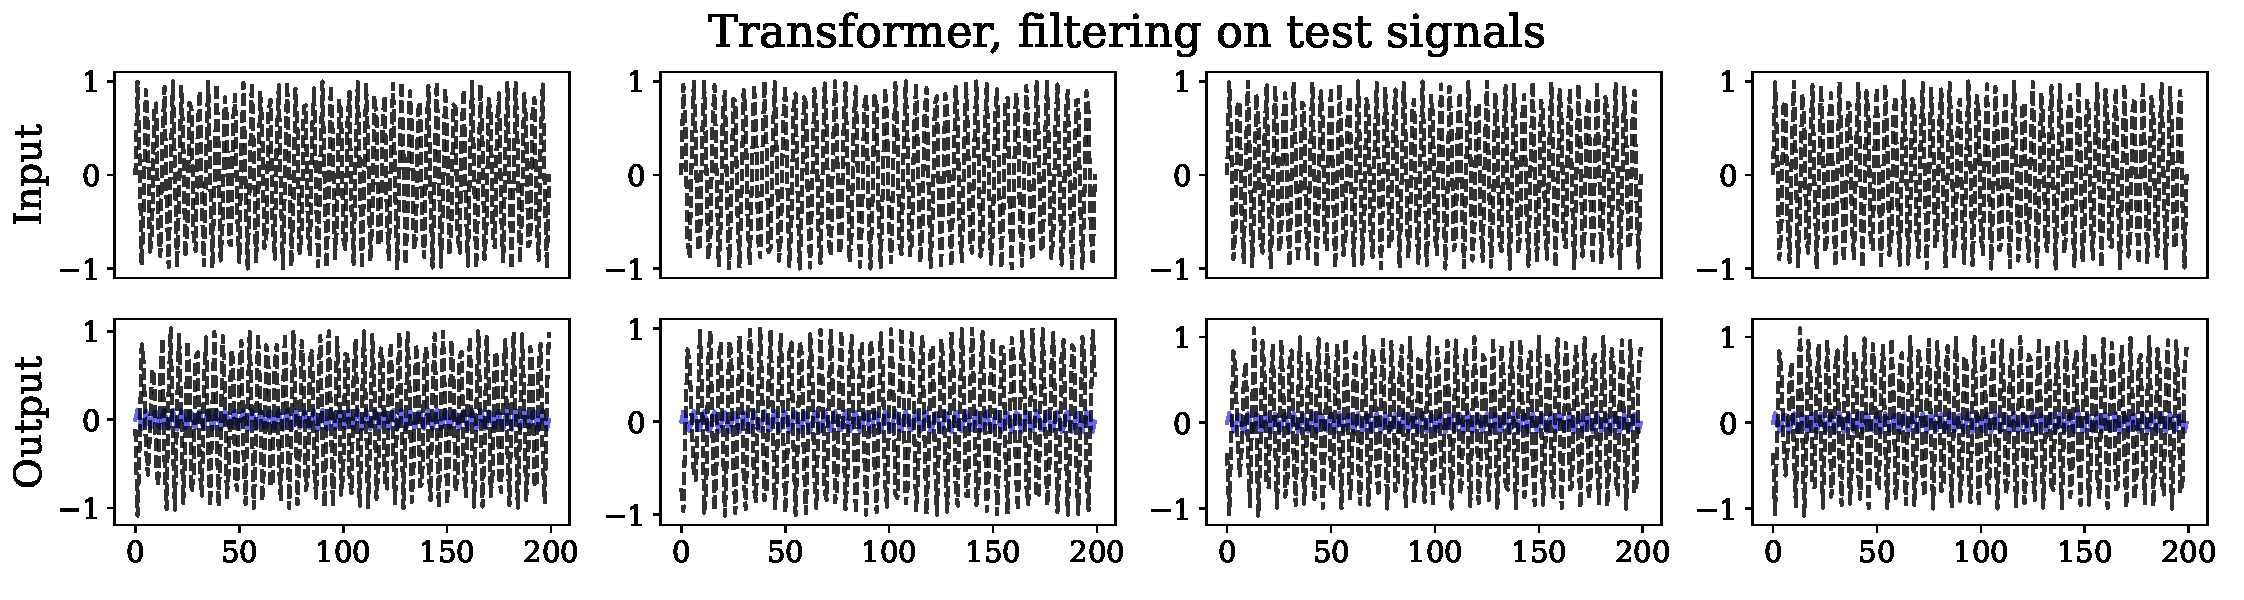
\includegraphics[width=0.99\columnwidth]{_ICLR2023_paper/figures/dsp_Transformer.pdf}
%     \caption{Testing the capability of different sequence--to--sequence models to approximate the input--output map of digital filters. In blue, we show the output signal filtered by each model. The ground--truth digital filter is a Butterworth of order $10$.}
%     \label{fig:dsp_synthetic}
% \end{figure}
% %




\subsection{Informer Forecasting}\label{appendix:informer_extended}

\textbf{Univariate long horizon forecasts with Informer splits.} Beyond the ETT datasets and horizons evaluated on in Table~\ref{tab:informer-s-long-original}, we also compare \ourmethod{} to alternative time series methods on the complete datasets and horizons used in the original Informer paper~\citep{zhou2021informer}. We compare against recent architectures which similarly evaluate on these settings, including ETSFormer~\citep{woo2022etsformer}, SCINet~\citep{liu2021time}, and Yformer~\citep{madhusudhanan2021yformer}, and other comparison methods found in the Informer paper, such as Reformer~\citep{kitaev2020reformer} and ARIMA.
\ourmethod{} obtains best results on 20 out of 25 settings, the most of any method.

\begin{table}[!t]
\caption{ \textbf{Univariate forecasting} results on Informer datasets. \textbf{Best} results in \textbf{bold}. \ourmethod{} obtains best MSE on 19 out of 25 and best MAE on 20 out of 25 dataset and horizon tasks.}
\resizebox{\linewidth}{!}{
\begin{tabular}{@{}c|cbcbcbcbcbcbcbcbcbcbcbcbc@{}}
% \begin{tabular}{@{}c|ccccccccccccccccccccccccc@{}}
\toprule
\multicolumn{2}{c}{Methods}        & \multicolumn{2}{c}{\textbf{\ourmethod{}}} & \multicolumn{2}{c}{ETSFormer}   & \multicolumn{2}{c}{SCINet} & \multicolumn{2}{c}{S4}          & \multicolumn{2}{c}{Yformer}     & \multicolumn{2}{c}{Informer} & \multicolumn{2}{c}{LogTrans} & \multicolumn{2}{c}{Reformer} & \multicolumn{2}{c}{N-BEATS} & \multicolumn{2}{c}{DeepAR} & \multicolumn{2}{c}{ARIMA} & \multicolumn{2}{c}{Prophet} \\ \midrule
\multicolumn{2}{c}{Metric}         & MSE                & MAE               & MSE            & MAE            & MSE          & MAE         & MSE            & MAE            & MSE            & MAE            & MSE           & MAE          & MSE           & MAE          & MSE           & MAE          & MSE          & MAE          & MSE          & MAE         & MSE         & MAE         & MSE          & MAE          \\ \midrule
\parbox[t]{2mm}{\multirow{5}{*}{\rotatebox[origin=c]{90}{ETTh1}}}   & 24  & \textbf{0.026}     & \textbf{0.124}    & 0.030          & 0.132          & 0.031        & 0.132       & 0.061          & 0.191          & 0.082          & 0.230          & 0.098         & 0.247        & 0.103         & 0.259        & 0.222         & 0.389        & 0.042        & 0.156        & 0.107        & 0.280       & 0.108       & 0.284       & 0.115        & 0.275        \\
\multicolumn{1}{c|}{}        & 48  & \textbf{0.038}     & \textbf{0.153}    & 0.041          & 0.154          & 0.051        & 0.173       & 0.079          & 0.220          & 0.139          & 0.308          & 0.158         & 0.319        & 0.167         & 0.328        & 0.284         & 0.445        & 0.065        & 0.200        & 0.162        & 0.327       & 0.175       & 0.424       & 0.168        & 0.330        \\
\multicolumn{1}{c|}{}        & 168 & 0.066              & 0.209             & \textbf{0.065} & \textbf{0.203} & 0.081        & 0.222       & 0.104          & 0.258          & 0.111          & 0.268          & 0.183         & 0.346        & 0.207         & 0.375        & 1.522         & 1.191        & 0.106        & 0.255        & 0.239        & 0.422       & 0.396       & 0.504       & 1.224        & 0.763        \\
\multicolumn{1}{c|}{}        & 336 & \textbf{0.069}     & \textbf{0.212}    & 0.071          & 0.215          & 0.094        & 0.242       & 0.080          & 0.229          & 0.195          & 0.365          & 0.222         & 0.387        & 0.230         & 0.398        & 1.860         & 1.124        & 0.127        & 0.284        & 0.445        & 0.552       & 0.468       & 0.593       & 1.549        & 1.820        \\
\multicolumn{1}{c|}{}        & 720 & \textbf{0.075}     & \textbf{0.226}    & 0.079          & 0.227          & 0.176        & 0.343       & 0.116          & 0.271          & 0.226          & 0.394          & 0.269         & 0.435        & 0.273         & 0.463        & 2.112         & 1.436        & 0.269        & 0.422        & 0.658        & 0.707       & 0.659       & 0.766       & 2.735        & 3.253        \\ \midrule
\parbox[t]{2mm}{\multirow{5}{*}{\rotatebox[origin=c]{90}{ETTh2}}}   & 24  & \textbf{0.064}     & \textbf{0.189}    & 0.087          & 0.232          & 0.070        & 0.194       & 0.095          & 0.234          & 0.082          & 0.221          & 0.093         & 0.240        & 0.102         & 0.255        & 0.263         & 0.437        & 0.078        & 0.210        & 0.098        & 0.263       & 3.554       & 0.445       & 0.199        & 0.381        \\
\multicolumn{1}{c|}{}        & 48  & \textbf{0.095}     & \textbf{0.230}    & 0.112          & 0.263          & 0.102        & 0.242       & 0.191          & 0.346          & 0.172          & 0.334          & 0.155         & 0.314        & 0.169         & 0.348        & 0.458         & 0.545        & 0.123        & 0.271        & 0.163        & 0.341       & 3.190       & 0.474       & 0.304        & 0.462        \\
\multicolumn{1}{c|}{}        & 168 & \textbf{0.144}     & \textbf{0.300}    & 0.169          & 0.325          & 0.157        & 0.311       & 0.167          & 0.333          & 0.174          & 0.337          & 0.232         & 0.389        & 0.246         & 0.422        & 1.029         & 0.879        & 0.244        & 0.393        & 0.255        & 0.414       & 2.800       & 0.595       & 2.145        & 1.068        \\
\multicolumn{1}{c|}{}        & 336 & \textbf{0.169}     & \textbf{0.333}    & 0.216          & 0.379          & 0.177        & 0.340       & 0.189          & 0.361          & 0.224          & 0.391          & 0.263         & 0.417        & 0.267         & 0.437        & 1.668         & 1.228        & 0.270        & 0.418        & 0.604        & 0.607       & 2.753       & 0.738       & 2.096        & 2.543        \\
\multicolumn{1}{c|}{}        & 720 & 0.188              & \textbf{0.352}    & 0.226          & 0.385          & 0.253        & 0.403       & \textbf{0.187} & 0.358          & 0.211          & 0.382          & 0.277         & 0.431        & 0.303         & 0.493        & 2.030         & 1.721        & 0.281        & 0.432        & 0.429        & 0.580       & 2.878       & 1.044       & 3.355        & 4.664        \\ \midrule
\parbox[t]{2mm}{\multirow{5}{*}{\rotatebox[origin=c]{90}{ETTm1}}}   & 24  & \textbf{0.010}     & \textbf{0.074}    & 0.013          & 0.084          & 0.019        & 0.088       & 0.024          & 0.117          & 0.024          & 0.118          & 0.030         & 0.137        & 0.065         & 0.202        & 0.095         & 0.228        & 0.031        & 0.117        & 0.091        & 0.243       & 0.090       & 0.206       & 0.120        & 0.290        \\
\multicolumn{1}{c|}{}        & 48  & \textbf{0.019}     & \textbf{0.101}    & 0.020          & 0.107          & 0.045        & 0.143       & 0.051          & 0.174          & 0.048          & 0.173          & 0.069         & 0.203        & 0.078         & 0.220        & 0.249         & 0.390        & 0.056        & 0.168        & 0.219        & 0.362       & 0.179       & 0.306       & 0.133        & 0.305        \\
\multicolumn{1}{c|}{}        & 96  & \textbf{0.026}     & \textbf{0.121}    & 0.030          & 0.132          & 0.072        & 0.198       & 0.086          & 0.229          & 0.143          & 0.311          & 0.194         & 0.372        & 0.199         & 0.386        & 0.920         & 0.767        & 0.095        & 0.234        & 0.364        & 0.496       & 0.272       & 0.399       & 0.194        & 0.396        \\
\multicolumn{1}{c|}{}        & 288 & \textbf{0.051}     & \textbf{0.176}    & 0.053          & 0.179          & 0.117        & 0.266       & 0.160          & 0.327          & 0.150          & 0.316          & 0.401         & 0.554        & 0.411         & 0.572        & 1.108         & 1.245        & 0.157        & 0.311        & 0.948        & 0.795       & 0.462       & 0.558       & 0.452        & 0.574        \\
\multicolumn{1}{c|}{}        & 672 & 0.078              & 0.220             & \textbf{0.075} & \textbf{0.214} & 0.180        & 0.328       & 0.292          & 0.466          & 0.305          & 0.476          & 0.512         & 0.644        & 0.598         & 0.702        & 1.793         & 1.528        & 0.207        & 0.370        & 2.437        & 1.352       & 0.639       & 0.697       & 2.747        & 1.174        \\ \midrule
\parbox[t]{2mm}{\multirow{5}{*}{\rotatebox[origin=c]{90}{Weather}}} & 24  & \textbf{0.088}     & \textbf{0.205}    & -              & -              & -            & -           & 0.125          & 0.254          & -              & -              & 0.117         & 0.251        & 0.136         & 0.279        & 0.231         & 0.401        & -            & -            & 0.128        & 0.274       & 0.219       & 0.355       & 0.302        & 0.433        \\
\multicolumn{1}{c|}{}        & 48  & \textbf{0.134}     & \textbf{0.258}    & -              & -              & -            & -           & 0.181          & 0.305          & -              & -              & 0.178         & 0.318        & 0.206         & 0.356        & 0.328         & 0.423        & -            & -            & 0.203        & 0.353       & 0.273       & 0.409       & 0.445        & 0.536        \\
\multicolumn{1}{c|}{}        & 168 & 0.221              & 0.349             & -              & -              & -            & -           & \textbf{0.198} & \textbf{0.333} & -              & -              & 0.266         & 0.398        & 0.309         & 0.439        & 0.654         & 0.634        & -            & -            & 0.293        & 0.451       & 0.503       & 0.599       & 2.441        & 1.142        \\
\multicolumn{1}{c|}{}        & 336 & \textbf{0.268}     & \textbf{0.380}    & -              & -              & -            & -           & 0.300          & 0.417          & -              & -              & 0.297         & 0.416        & 0.359         & 0.484        & 1.792         & 1.093        & -            & -            & 0.585        & 0.644       & 0.728       & 0.730       & 1.987        & 2.468        \\
\multicolumn{1}{c|}{}        & 720 & 0.345              & 0.451             & -              & -              & -            & -           & \textbf{0.245} & \textbf{0.375} & -              & -              & 0.359         & 0.466        & 0.388         & 0.499        & 2.087         & 1.534        & -            & -            & 0.499        & 0.596       & 1.062       & 0.943       & 3.859        & 1.144        \\ \midrule
\parbox[t]{2mm}{\multirow{5}{*}{\rotatebox[origin=c]{90}{ECL} }}    & 48  & \textbf{0.184}     & \textbf{0.306}    & -              & -              & -            & -           & 0.222          & 0.350          & 0.194          & 0.322          & 0.239         & 0.359        & 0.280         & 0.429        & 0.971         & 0.884        & -            & -            & 0.204        & 0.357       & 0.879       & 0.764       & 0.524        & 0.595        \\
\multicolumn{1}{c|}{}        & 168 & \textbf{0.250}     & \textbf{0.353}    & -              & -              & -            & -           & 0.331          & 0.421          & 0.260          & 0.361          & 0.447         & 0.503        & 0.454         & 0.529        & 1.671         & 1.587        & -            & -            & 0.315        & 0.436       & 1.032       & 0.833       & 2.725        & 1.273        \\
\multicolumn{1}{c|}{}        & 336 & 0.288              & 0.382             & -              & -              & -            & -           & 0.328          & 0.422          & \textbf{0.269} & \textbf{0.375} & 0.489         & 0.528        & 0.514         & 0.563        & 3.528         & 2.196        & -            & -            & 0.414        & 0.519       & 1.136       & 0.876       & 2.246        & 3.077        \\
\multicolumn{1}{c|}{}        & 720 & \textbf{0.355}     & \textbf{0.446}    & -              & -              & -            & -           & 0.428          & 0.494          & 0.427          & 0.479          & 0.540         & 0.571        & 0.558         & 0.609        & 4.891         & 4.047        & -            & -            & 0.563        & 0.595       & 1.251       & 0.933       & 4.243        & 1.415        \\
\multicolumn{1}{c|}{}        & 960 & \textbf{0.393}     & \textbf{0.478}    & -              & -              & -            & -           & 0.432          & 0.497          & 0.595          & 0.573          & 0.582         & 0.608        & 0.624         & 0.645        & 7.019         & 5.105        & -            & -            & 0.657        & 0.683       & 1.370       & 0.982       & 6.901        & 4.260        \\ \midrule
\multicolumn{2}{c}{Count}          & \textbf{19}        & \textbf{20}       & 2              & 2              & 0            & 0           & 3              & 2              & 1              & 1              & 0             & 0            & 0             & 0            & 0             & 0            & 0            & 0            & 0            & 0           & 0           & 0           & 0            & 0            \\ \bottomrule
\end{tabular}
}
\label{tab:informer-s-long-original}
\end{table}


% \begin{table}[!t]
% \caption{ \textbf{Univariate forecasting} results on Informer datasets. \textbf{Best} results in \textbf{bold}. \ourmethod{} obtains best MSE on 19 out of 25 and best MAE on 20 out of 25 dataset and horizon tasks.}
% \resizebox{\linewidth}{!}{
% \begin{tabular}{@{}c|cbcbcbcbcbcbcbcbcbcbcbcbc@{}}
% \toprule
% \multicolumn{2}{c}{Methods}                         & \multicolumn{2}{c}{\textbf{\ourmethod{}}}   & \multicolumn{2}{c}{ETSFormer}   & \multicolumn{2}{c}{SCINet} & \multicolumn{2}{c}{S4}          & \multicolumn{2}{c}{Yformer}     & \multicolumn{2}{c}{Informer} & \multicolumn{2}{c}{LogTrans} & \multicolumn{2}{c}{Reformer} & \multicolumn{2}{c}{DeepAR} & \multicolumn{2}{c}{ARIMA} & \multicolumn{2}{c}{Prophet} \\ \midrule
% \multicolumn{2}{c}{Metric}                          & MSE            & MAE            & MSE            & MAE            & MSE          & MAE         & MSE            & MAE            & MSE            & MAE            & MSE           & MAE          & MSE           & MAE          & MSE           & MAE          & MSE          & MAE         & MSE         & MAE         & MSE          & MAE          \\ \midrule
% \parbox[t]{2mm}{\multirow{5}{*}{\rotatebox[origin=c]{90}{ETTh1}}}   & 24  & \textbf{0.026} & \textbf{0.124} & 0.030          & 0.132          & 0.031        & 0.132       & 0.061          & 0.191          & 0.082          & 0.230          & 0.098         & 0.247        & 0.103         & 0.259        & 0.222         & 0.389        & 0.107        & 0.280       & 0.108       & 0.284       & 0.115        & 0.275        \\
% \multicolumn{1}{c|}{}                         & 48  & \textbf{0.038} & \textbf{0.153} & 0.041          & 0.154          & 0.051        & 0.173       & 0.079          & 0.220          & 0.139          & 0.308          & 0.158         & 0.319        & 0.167         & 0.328        & 0.284         & 0.445        & 0.162        & 0.327       & 0.175       & 0.424       & 0.168        & 0.330        \\
% \multicolumn{1}{c|}{}                         & 168 & 0.066          & 0.209          & \textbf{0.065} & \textbf{0.203} & 0.081        & 0.222       & 0.104          & 0.258          & 0.111          & 0.268          & 0.183         & 0.346        & 0.207         & 0.375        & 1.522         & 1.191        & 0.239        & 0.422       & 0.396       & 0.504       & 1.224        & 0.763        \\
% \multicolumn{1}{c|}{}                         & 336 & \textbf{0.069} & \textbf{0.212} & 0.071          & 0.215          & 0.094        & 0.242       & 0.080          & 0.229          & 0.195          & 0.365          & 0.222         & 0.387        & 0.230         & 0.398        & 1.860         & 1.124        & 0.445        & 0.552       & 0.468       & 0.593       & 1.549        & 1.820        \\
% \multicolumn{1}{c|}{}                         & 720 & \textbf{0.075} & \textbf{0.226} & 0.079          & 0.227          & 0.176        & 0.343       & 0.116          & 0.271          & 0.226          & 0.394          & 0.269         & 0.435        & 0.273         & 0.463        & 2.112         & 1.436        & 0.658        & 0.707       & 0.659       & 0.766       & 2.735        & 3.253        \\ \midrule
% \parbox[t]{2mm}{\multirow{5}{*}{\rotatebox[origin=c]{90}{ETTh2}}}   & 24  & \textbf{0.064} & \textbf{0.189} & 0.087          & 0.232          & 0.070        & 0.194       & 0.095          & 0.234          & 0.082          & 0.221          & 0.093         & 0.240        & 0.102         & 0.255        & 0.263         & 0.437        & 0.098        & 0.263       & 3.554       & 0.445       & 0.199        & 0.381        \\
% \multicolumn{1}{c|}{}                         & 48  & \textbf{0.095} & \textbf{0.230} & 0.112          & 0.263          & 0.102        & 0.242       & 0.191          & 0.346          & 0.172          & 0.334          & 0.155         & 0.314        & 0.169         & 0.348        & 0.458         & 0.545        & 0.163        & 0.341       & 3.190       & 0.474       & 0.304        & 0.462        \\
% \multicolumn{1}{c|}{}                         & 168 & \textbf{0.144} & \textbf{0.300} & 0.169          & 0.325          & 0.157        & 0.311       & 0.167          & 0.333          & 0.174          & 0.337          & 0.232         & 0.389        & 0.246         & 0.422        & 1.029         & 0.879        & 0.255        & 0.414       & 2.800       & 0.595       & 2.145        & 1.068        \\
% \multicolumn{1}{c|}{}                         & 336 & \textbf{0.169} & \textbf{0.333} & 0.216          & 0.379          & 0.177        & 0.340       & 0.189          & 0.361          & 0.224          & 0.391          & 0.263         & 0.417        & 0.267         & 0.437        & 1.668         & 1.228        & 0.604        & 0.607       & 2.753       & 0.738       & 2.096        & 2.543        \\
% \multicolumn{1}{c|}{}                         & 720 & \textbf{0.188} & \textbf{0.352} & 0.226          & 0.385          & 0.253        & 0.403       & 0.187          & 0.358          & 0.211          & 0.382          & 0.277         & 0.431        & 0.303         & 0.493        & 2.030         & 1.721        & 0.429        & 0.580       & 2.878       & 1.044       & 3.355        & 4.664        \\ \midrule
% \parbox[t]{2mm}{\multirow{5}{*}{\rotatebox[origin=c]{90}{ETTm1}}}   & 24  & \textbf{0.010} & \textbf{0.074} & 0.013          & 0.084          & 0.019        & 0.088       & 0.024          & 0.117          & 0.024          & 0.118          & 0.030         & 0.137        & 0.065         & 0.202        & 0.095         & 0.228        & 0.091        & 0.243       & 0.090       & 0.206       & 0.120        & 0.290        \\
% \multicolumn{1}{c|}{}                         & 48  & \textbf{0.019} & \textbf{0.101} & 0.020          & 0.107          & 0.045        & 0.143       & 0.051          & 0.174          & 0.048          & 0.173          & 0.069         & 0.203        & 0.078         & 0.220        & 0.249         & 0.390        & 0.219        & 0.362       & 0.179       & 0.306       & 0.133        & 0.305        \\
% \multicolumn{1}{c|}{}                         & 96  & \textbf{0.026} & \textbf{0.121} & 0.030          & 0.132          & 0.072        & 0.198       & 0.086          & 0.229          & 0.143          & 0.311          & 0.194         & 0.372        & 0.199         & 0.386        & 0.920         & 0.767        & 0.364        & 0.496       & 0.272       & 0.399       & 0.194        & 0.396        \\
% \multicolumn{1}{c|}{}                         & 288 & \textbf{0.051} & \textbf{0.176} & 0.053          & 0.179          & 0.117        & 0.266       & 0.160          & 0.327          & 0.150          & 0.316          & 0.401         & 0.554        & 0.411         & 0.572        & 1.108         & 1.245        & 0.948        & 0.795       & 0.462       & 0.558       & 0.452        & 0.574        \\
% \multicolumn{1}{c|}{}                         & 672 & 0.078          & 0.220          & \textbf{0.075} & \textbf{0.214} & 0.180        & 0.328       & 0.292          & 0.466          & 0.305          & 0.476          & 0.512         & 0.644        & 0.598         & 0.702        & 1.793         & 1.528        & 2.437        & 1.352       & 0.639       & 0.697       & 2.747        & 1.174        \\ \midrule
% \parbox[t]{2mm}{\multirow{5}{*}{\rotatebox[origin=c]{90}{Weather}}}  & 24  & \textbf{0.088} & \textbf{0.205} & -              & -              & -            & -           & 0.125          & 0.254          & -              & -              & 0.117         & 0.251        & 0.136         & 0.279        & 0.231         & 0.401        & 0.128        & 0.274       & 0.219       & 0.355       & 0.302        & 0.433        \\
% \multicolumn{1}{c|}{}                         & 48  & \textbf{0.134} & \textbf{0.258} & -              & -              & -            & -           & 0.181          & 0.305          & -              & -              & 0.178         & 0.318        & 0.206         & 0.356        & 0.328         & 0.423        & 0.203        & 0.353       & 0.273       & 0.409       & 0.445        & 0.536        \\
% \multicolumn{1}{c|}{}                         & 168 & 0.221          & 0.349          & -              & -              & -            & -           & \textbf{0.198} & \textbf{0.333} & -              & -              & 0.266         & 0.398        & 0.309         & 0.439        & 0.654         & 0.634        & 0.293        & 0.451       & 0.503       & 0.599       & 2.441        & 1.142        \\
% \multicolumn{1}{c|}{}                         & 336 & \textbf{0.268} & \textbf{0.380} & -              & -              & -            & -           & 0.300          & 0.417          & -              & -              & 0.297         & 0.416        & 0.359         & 0.484        & 1.792         & 1.093        & 0.585        & 0.644       & 0.728       & 0.730       & 1.987        & 2.468        \\
% \multicolumn{1}{c|}{}                         & 720 & 0.345          & 0.451          & -              & -              & -            & -           & \textbf{0.245} & \textbf{0.375} & -              & -              & 0.359         & 0.466        & 0.388         & 0.499        & 2.087         & 1.534        & 0.499        & 0.596       & 1.062       & 0.943       & 3.859        & 1.144        \\ \midrule
% \parbox[t]{2mm}{\multirow{5}{*}{\rotatebox[origin=c]{90}{ECL}}}      & 48  & \textbf{0.184} & \textbf{0.306} & -              & -              & -            & -           & 0.222          & 0.350          & 0.194          & 0.322          & 0.239         & 0.359        & 0.280         & 0.429        & 0.971         & 0.884        & 0.204        & 0.357       & 0.879       & 0.764       & 0.524        & 0.595        \\
% \multicolumn{1}{c|}{}                         & 168 & \textbf{0.250} & \textbf{0.353} & -              & -              & -            & -           & 0.331          & 0.421          & 0.260          & 0.361          & 0.447         & 0.503        & 0.454         & 0.529        & 1.671         & 1.587        & 0.315        & 0.436       & 1.032       & 0.833       & 2.725        & 1.273        \\
% \multicolumn{1}{c|}{}                         & 336 & 0.288          & 0.382          & -              & -              & -            & -           & 0.328          & 0.422          & \textbf{0.269} & \textbf{0.375} & 0.489         & 0.528        & 0.514         & 0.563        & 3.528         & 2.196        & 0.414        & 0.519       & 1.136       & 0.876       & 2.246        & 3.077        \\
% \multicolumn{1}{c|}{}                         & 720 & \textbf{0.355} & \textbf{0.446} & -              & -              & -            & -           & 0.428          & 0.494          & 0.427          & 0.479          & 0.540         & 0.571        & 0.558         & 0.609        & 4.891         & 4.047        & 0.563        & 0.595       & 1.251       & 0.933       & 4.243        & 1.415        \\
% \multicolumn{1}{c|}{}                         & 960 & \textbf{0.393} & \textbf{0.478} & -              & -              & -            & -           & 0.432          & 0.497          & 0.595          & 0.573          & 0.582         & 0.608        & 0.624         & 0.645        & 7.019         & 5.105        & 0.657        & 0.683       & 1.370       & 0.982       & 6.901        & 4.260        \\ \midrule
% \multicolumn{2}{c}{Count}                           & \textbf{20}             & \textbf{20}             & 2              & 2              & 0            & 0           & 2              & 2              & 1              & 1              & 0             & 0            & 0             & 0            & 0             & 0            & 0            & 0           & 0           & 0           & 0            & 0            \\ \bottomrule
% \end{tabular}
% }
% \label{tab:informer-s-long-original}
% \end{table}




\textbf{Multivariate signals.} We additionally compare the performance of \ourmethod{} to state-of-the-art comparison methods on ETT multivariate settings. We focus on horizon length $720$, the longest evaluated in prior works. In Table \ref{tab:informer-m-long}, we find \ourmethod{} is competitive with NLinear, which achieves best performance among compparison methods. \ourmethod{} also notably outperforming S4 by large margins, supporting the companion matrix representation once more.   

% Please add the following required packages to your document preamble:
% \usepackage{booktabs}
\begin{table}[!t]
\caption{\textbf{Multivariate forecasting} results on Informer datasets. \textbf{Best} results in \textbf{bold}. \ourmethod{} obtains MSE and MAE competitive with NLinear, the prior state-of-the-art.}
\resizebox{\linewidth}{!}{
\begin{tabular}{@{}ccbcbcbcbcbcbcbc@{}}
\toprule
\multicolumn{2}{c}{Methods}      & \multicolumn{2}{c}{\ourmethod{}}   & \multicolumn{2}{c}{NLinear}     & \multicolumn{2}{c}{FiLM} & \multicolumn{2}{c}{S4} & \multicolumn{2}{c}{FEDformer} & \multicolumn{2}{c}{Autoformer} & \multicolumn{2}{c}{Informer} \\ \midrule
\multicolumn{2}{c}{Metric}       & MSE            & MAE            & MSE            & MAE            & MSE         & MAE        & MSE        & MAE       & MSE           & MAE           & MSE            & MAE           & MSE           & MAE          \\ \midrule
\multicolumn{1}{c|}{ETTh1} & 720 & 0.499          & 0.480           & \textbf{0.440}  & \textbf{0.453} & 0.465       & 0.472      & 1.074      & 0.814     & 0.506         & 0.507         & 0.514          & 0.512         & 1.181         & 0.865        \\
\multicolumn{1}{c|}{ETTh2} & 720 & 0.402          & \textbf{0.434} & \textbf{0.394} & 0.436          & 0.439       & 0.456      & 2.973      & 1.333     & 0.463         & 0.474         & 0.515          & 0.511         & 3.647         & 1.625        \\
\multicolumn{1}{c|}{ETTm1} & 720 & \textbf{0.408} & \textbf{0.415} & 0.433          & 0.422          & 0.420       & 0.420      & 0.738      & 0.655     & 0.543         & 0.49          & 0.671          & 0.561         & 1.166         & 0.823        \\
\multicolumn{1}{c|}{ETTm2} & 720 & \textbf{0.358} & \textbf{0.378} & 0.368 & 0.384 & 0.393       & 0.422      & 2.074      & 1.074     & 0.421         & 0.415         & 0.433          & 0.432         & 3.379         & 1.338        \\ \bottomrule
\end{tabular}
}
\label{tab:informer-m-long}
\end{table}


\subsection{Monash Forecasting} \label{app:monash_exps}

We report the results across all datasets in Table \ref{tab:monash}. We also investigate the performance of models by aggregating datasets based on common characteristics. Concretely, we generate sets of tasks\footnote{A task can belong to multiple splits, resulting in overlapping splits. For example, a task can involve both long context as well as long forecasting horizon.} based on the following properties: 
\begin{itemize}
    \item \textit{Large dataset:} the dataset contains more than $2000$ effective training samples.
    \item \textit{Long context:} the models are provided a context of length greater than $20$ as input.
    \item \textit{Long horizon:} and the models are asked to forecast longer than $20$ steps in the future.
\end{itemize} 
Figure \ref{fig:monash_rankings} shows the average $x/13$ model ranking in terms of test RMSE across splits. We contextualize \ourmethod{} results with best classical and deep learning methods (TBATS and DeepAR). \ourmethod{} relative performance is noticeably higher when context and forecasting horizons are longer, and when a larger number of samples is provided during training. 


%\begin{wrapfigure}[23]{r}{0.55\textwidth}
\begin{figure}[ht]
    \centering
    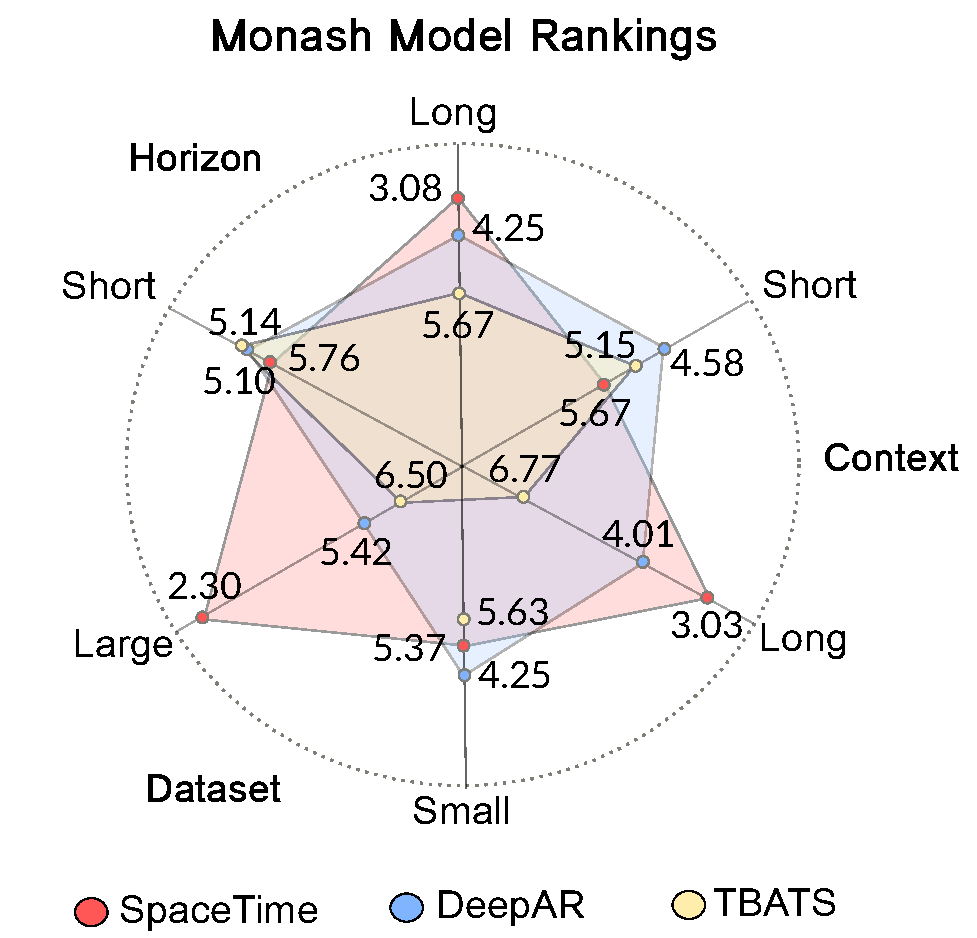
\includegraphics[width=0.5\linewidth]{_ICLR2023_paper/figures/monash_rankings2.pdf}
    \caption{ Relative test RMSE rankings ($*/13$ models) across different slices of the $33$ datasets in the Monash repository \citep{godahewa2021monash}. \ourmethod{} sets best overall ranking across all tasks and is significantly more accurate on tasks involving long forecast horizon and larger number of training samples.}
    \label{fig:monash_rankings}
\end{figure}
%\end{wrapfigure}


\subsection{ECG Classification}\label{appendix:ecg_results}

In addition to our results table in the main paper, we also provide the mean and standard deviations of the two models we ran in house (\ourmethod{} and S4) in Table \ref{tab:ecg_stats}.

\begin{table}[H]
    \centering
    \caption{ \textbf{ECG statement classification} on PTB-XL (100 Hz version). We report the mean and standard deviation over three random seeds for the three methods we ran in house.}
    \label{tab:ecg_stats}
    \begin{tabular}{@{}lcccccc@{}}
\toprule
Task AUROC & All            & Diag           & Sub-diag       & Super-diag     & Form           & Rhythm         \\ \midrule
\ourmethod{}            & $93.6 (0.13)$   & $94.1 (0.12)$ & $93.3(0.34)$ & $92.9 (0.09)$ & $88.3(0.63)$          & $96.7 (0.05)$    \\
S4    & $93.8 (0.38)$ & $93.9 (0.15)$  & $92.9 (0.11)$ & $93.1 (0.07)$    & $89.5 (0.66)$  & $97.7 (0.04)$ \\
Transformer    & $85.7 (0.30)$ & $87.6 (0.41)$  & $88.2 (0.20)$ & $88.7 (0.28)$    & $77.1 (0.45)$  & $83.1 (0.72)$ \\
\bottomrule
\end{tabular}
    
\end{table}


\subsection{Efficiency Results}

We additionally empirically validate that \ourmethod{} trains in near-linear time with horizon sequence length. We also use synthetic data, scaling horizon from $1 - 1000$. 

\begin{figure}[H]
  \centering
    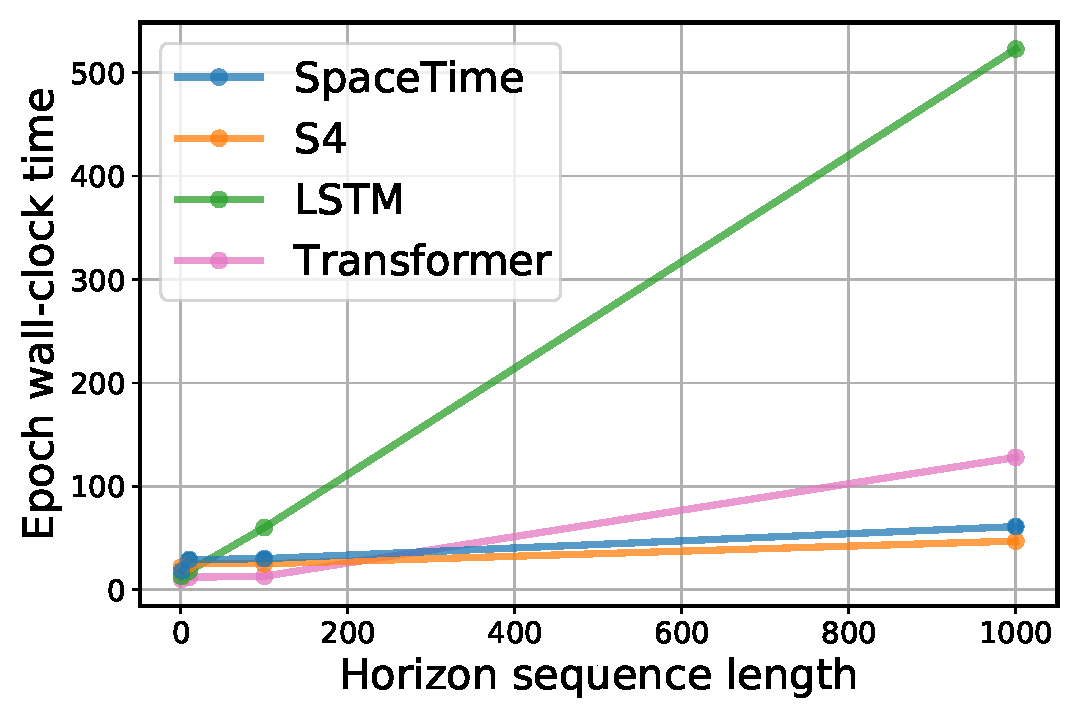
\includegraphics[width=0.5\textwidth]{_ICLR2023_paper/figures/speed_benchmark_horizon.pdf}
  \caption{Training wall-clock time versus horizon length for \ourmethod{}, S4, LSTM, and Transformer. }
  \label{fig:horizon_efficiency} 
\end{figure}


\subsection{\ourmethod{} Ablations}\label{appendix:ablations}
To better understand how the proposed \ourmethod{} SSMs lead to the improved empirical performance, we include ablations on the individual closed-loop forecasting SSM (Section~\ref{sec:forecasting_ssm}) and preprocessing SSMs (Section~\ref{sec:preprocessing_ssms}). 

\subsubsection{Closed-loop Forecasting SSM}\label{appendix:ablations_closed_loop_ssm}
To study how the closed-loop SSM improves long horizon forecasting accuracy, we remove the closed-loop SSM component in our default \ourmethod{} forecasting architecture (\cf{} Appendix~\ref{appendix:architectures}, and compare the default \ourmethod{} with one without any closed-loop SSMs on Informer forecasting tasks. For models without closed-loop SSMs, we replace the last layer with the standard ``open-loop'' SSM framework in Section~\ref{sec:method_spacetime_layer}), and keep all other layers the same. Finally, for baseline comparison against another SSM without the closed-loop component, we compare against S4. 

In Table~\ref{tab:ablation_results_closed_loop_ssm}, we report standardized MSE on Informer ETT datasets. Adding the closed-loop SSM consistently improves forecasting accuracy, on average lowering relative MSE by 33.2\%. Meanwhile, even without the closed-loop SSM, \ourmethod{} outperforms S4, again suggesting that the companion matrix parameterization is beneficial for autoregressive time series forecasting. 

\begin{table}[H]
    \centering
    \caption{ \textbf{Closed-loop SSM Ablation} We ablate the closed-loop SSM component in \ourmethod{}, comparing against the prior S4 SSM on four Informer time series forecasting tasks. Removing the closed-loop SSM consistently hurts forecasting accuracy for \ourmethod{}. }
    \label{tab:ablation_results_closed_loop_ssm}
    \begin{tabular}{@{}lbcbcbcbc@{}}
\toprule
                            & \multicolumn{2}{c}{ETTh1 (720)} & \multicolumn{2}{c}{ETTh2 (720)} & \multicolumn{2}{c}{ETTm1 (720)} & \multicolumn{2}{c}{ETTm2 (720)} \\ \cmidrule(l){2-9} 
Method / Ablation                      & MSE            & MAE            & MSE            & MAE            & MSE            & MAE            & MSE            & MAE            \\ \midrule
\ourmethod{}                & 0.076          & 0.222          & 0.188          & 0.352          & 0.074          & 0.213          & 0.166          & 0.318          \\
\ourmethod{} No Closed-loop & 0.114          & 0.271          & 0.278          & 0.431          & 0.156          & 0.310          & 0.213          & 0.365          \\
S4 (No Closed-loop)         & 0.190          & 0.355          & 0.630          & 0.662          & 0.254          & 0.433          & 0.482          & 0.567          \\ \bottomrule
\end{tabular}
    
\end{table}

\subsubsection{Preprocessing SSM}\label{appendix:ablations_preprocessing_ssm}

To study how the preprocessing SSM improves long horizon forecasting accuracy, we next compare how \ourmethod{} performs with and without the weight-initializing preprocessing SSMs introduced in Section~\ref{sec:preprocessing_ssms}. We compare the default \ourmethod{} architecture (Table~\ref{tab:spacetime_forecasting_arch} with (1) replacing the preprocessing SSMs with randomly initialized default companion SSMs, and (2) removing the preprocessing SSMs altogether. For the former, we preserve the number of layers, but now train the first-layer SSM weights. For the latter, there is one-less layer, but the same number of trainable parameters (as we fix and freeze the weights for each preprocessing SSM). 


In Table~\ref{tab:ablation_results_preprocessing_ssm}, we report standardized MSE on Informer ETT datasets. We find fixing the first layer SSMs of a \ourmethod{} network to preprocessing SSMs consistently improves forecasting performance, achieving 4.55\% lower MSE on average than the ablation with just trainable companion matrices. Including the preprocessing layer also improves MSE by 9.26\% on average compared to removing the layer altogether. These results suggest that preprocessing SSMs are beneficial for time series forecasting, \eg{} by performing classic time series modeling techniques on input data. Unlike other approaches, \ourmethod{} is able to flexibly and naturally incorporate these operations into its network layers via simple weight initializations of the same general companion SSM structure. 


\begin{table}[H]
    \centering
    \caption{ \textbf{Preprocessing SSM Ablation} We ablate the preprocessing SSM layer in \ourmethod{}, comparing against either replacing the SSMs with companion SSMs (Companion) or removing the layer (Removed). Including preprocessing SSMs consistently improves forecasting accuracy. }
    \label{tab:ablation_results_preprocessing_ssm}
\resizebox{\linewidth}{!}{
\begin{tabular}{@{}lbcbcbcbc@{}}
\toprule
                                           & \multicolumn{2}{c}{ETTh1 (720)} & \multicolumn{2}{c}{ETTh2 (720)} & \multicolumn{2}{c}{ETTm1 (720)} & \multicolumn{2}{c}{ETTm2 (720)} \\ \cmidrule(l){2-9} 
Method / Ablation                          & MSE            & MAE            & MSE            & MAE            & MSE            & MAE            & MSE            & MAE            \\ \midrule
SpaceTime                                  & 0.076          & 0.222          & 0.188          & 0.352          & 0.074          & 0.213          & 0.166          & 0.318          \\
SpaceTime No Preprocessing (Companion)     & 0.076          & 0.224          & 0.194          & 0.358          & 0.079          & 0.218          & 0.182          & 0.336          \\
SpaceTime No Preprocessing (Removed) & 0.078          & 0.227          & 0.204          & 0.367          & 0.087          & 0.232          & 0.188          & 0.326          \\ \bottomrule
\end{tabular}
}    
\end{table}


\subsection{\ourmethod{} Architectures}\label{appendix:architectures}

We provide the specific \ourmethod{} architecture configurations used for forecasting and classification tasks. Each configuration follows the general architecture presented in Section~\ref{sec:expressive_ssm_layer} and Figure~\ref{fig:arch_overview}, and consists of repeated Multi-SSM \ourmethod{} layers. We first provide additional details on specific instantiations of the companion SSMs we use in our models, \eg{} how we instantiate preprocessing SSMs to recover specific techniques (Section~\ref{sec:preprocessing_ssms}). We then include the layer-specific details of the number and type of SSM used in each network. 

\subsubsection{Specific SSM parameterizations}\label{appendix:specific_ssm_parameterizations}
In Section~\ref{sec:expressive_ssm_with_companion}, we described the general form of the companion SSM used in this work. By default, for any individual SSM we learn the $a$ column in $\zA$ and the vectors $\zB, \zC$ as trainable parameters in a neural net module. We refer to these SSMs specifically as \textbf{companion SSMs}. 

In addition, as discussed in Sections~\ref{sec:expressive_ssm_with_companion} and ~\ref{sec:preprocessing_ssms}, we can also fix $a$, $\zB$, or $\zC$ to specific values to recover useful operations when computing the SSM outputs. We describe specific instantiations of the companion SSM used in our models below (with dimensionality referring to one SSM). 

\header{Shift SSM}
We fix the $\boldsymbol{a}$ vector in the companion state matrix $\zA \in \mathbb{R}^{d \times d}$ to the $\boldsymbol{0}$ vector $\in \mathbb{R}^d$, such that $\zA$ is the shift matrix (see Eq.~\ref{eq:shift_matrix_example} for an example). This is a generalization of a 1-D ``sliding window'' convolution with fixed kernel size equal to SSM state dimension $d$. To see how, note that if $\zB$ is also fixed to the first basis vector $\boldsymbol{e_1} \in \mathbb{R}^{d \times 1}$, then this exactly recovers a 1-D convolution with kernel determined by $\zC$.

\header{Differencing SSM}
As a specific version of the preprocessing SSM discussed in Section~\ref{sec:preprocessing_ssms}, we fix $\boldsymbol{a} = \boldsymbol{0}$, $\zB = \boldsymbol{e_1}$, and set $\zC$ to recover various order differencing when computing the SSM, \ie{}
% \begin{align}
% \zC = \bmatrix 1 & -1 & 0 & \ldots & 0}\;\;\;\text{(1st-order differencing)}
% \end{align}
\begin{align}
    \zC &= 
    \begin{bmatrix}
    1 & \phantom{-}0 & 0 & \phantom{-}0 & 0 & \ldots & 0 \\
    \end{bmatrix}
    \;\;\;\;\;\;
    \begin{matrix}
    \hfill\text{(0-order differencing, \ie{} an identity function)} \\
    \end{matrix} \\
    \zC &= 
    \begin{bmatrix}
    1 & -1 & 0 & \phantom{-}0 & 0 & \ldots & 0 \\
    \end{bmatrix}
    \;\;\;\;\;\;
    \begin{matrix}
    \hfill\text{(1st-order differencing)} \\
    \end{matrix} \\
    \zC &= 
    \begin{bmatrix}
    1 & -2 & 1 & \phantom{-}0 & 0 & \ldots & 0 \\
    \end{bmatrix}
    \;\;\;\;\;\;
    \begin{matrix}
    \hfill\text{ (2nd-order differencing)} \\
    \end{matrix} \\
    \zC &= 
    \begin{bmatrix}
    1 & -3 & 3 & -1 & 0 & \ldots & 0 \\
    \end{bmatrix}
    \;\;\;\;\;\;
    \begin{matrix}
    \hfill\text{ (3rd-order differencing)} \\
    \end{matrix}
\end{align}
 In this work, we only use the above 0, 1st, 2nd, or 3rd-order differencing instantiations. With multiple differencing SSMs in a multi-SSM \ourmethod{} layer, we initialize differencing SSMs by running through the orders repeatedly in sequence. For example, given five differencing SSMs, the first four SSMs perform 0, 1st, 2nd, and 3rd-order differencing respectively, while the fifth performs 0-order differencing again.

\header{Moving Average Residual (MA residual) SSM}
As another version of the preprocessing SSM, we can fix $\boldsymbol{a} = \boldsymbol{0}$, $\zB = \boldsymbol{e_1}$, and set $\zC$ such that the SSM outputs sample residuals from a moving average applied over the input sequence. For an $n$-order moving average, we compute outputs with $\zC$ specified as
\begin{align}
    \zC &= 
    \begin{bmatrix}
    1 - 1/n, & -1/n, & \ldots & -1/n, & 0 & \ldots & 0 \\
    \end{bmatrix}
    \;\;\;\;\;\;
    \begin{matrix}
    \hfill\text{($n$-order moving average residual)} \\
    \end{matrix}
\end{align}
For each MA residual SSM, we randomly initialize the order by uniform-randomly sampling an integer in the range $[4, d]$, where $d$ is again the state-space dimension size (recall $\zC \in \mathbb{R}^{1 \times d}$). We pick $4$ as a heuristic which was not finetuned; we leave additional optimization here for further work.

\subsubsection{Task-specific \ourmethod{} Architectures}\label{appendix:specific_spacetime_architectures}

Here we provide layer-level details on the \ourmethod{} networks used in this work. For each task, we describe number of layers, number of SSMs per layer, state-space dimension (fixed for all SSMs in a network), and which SSMs are used in each layer. 

Expanding on this last detail, as previously discussed in Section~\ref{sec:method_spacetime_layer}, in each \ourmethod{} layer we can specify multiple SSMs in each layer, computing their outputs in parallel to produce a multidimensional output that is fed as the input to the next \ourmethod{} layer. The ``types'' of SSMs do not all have to be the same per layer, and we list the type (companion, shift, differencing, MA residual) and closed-loop designation (standard, closed-loop) of the SSMs in each layer below.

For an additional visual overview of a \ourmethod{} network, please refer back to Figure~\ref{fig:arch_overview}.

\header{Forecasting: Informer and Monash}
We describe the architecture in Table~\ref{tab:spacetime_forecasting_arch}. We treat the first \ourmethod{} layer as ``preprocessing'' layer, which performs differencing and moving average residual operations on the input sequence. We treat the last \ourmethod{} layer as a ``forecasting'' layer, which autoregressively outputs future horizon predictions given the second-to-last layer's outputs as an input sequence.

% \[
% \begin{aligned}
%     \begin{matrix}
%     \text{\phantom{-}} \\
%     \end{matrix}
%     \\
%     &
%     \begin{bmatrix}
%     \text{\phantom{-} Differencing \phantom{-}}   \\ \text{(standard)} \\
%     \end{bmatrix}
%     \times 192 
%     \\
%     \begin{matrix}
%     \text{\phantom{-}} \\
%     \end{matrix}
%     \\
%     &
%     &
%     \begin{bmatrix}
%     \text{\phantom{-} MA Residual\phantom{-} }   \\ \text{(standard)} \\
%     \end{bmatrix}
%      \times 64 
%      \\
%      \begin{matrix}
%     \text{\phantom{-}} \\
%     \end{matrix}
%     \\
% \end{aligned}
% \]

% \[
% \begin{aligned}
%     \begin{matrix}
%     \text{\phantom{-}} \\
%     \end{matrix}
%     \\
%     &
%     \begin{bmatrix}
%     \text{\phantom{-} Differencing \phantom{-}}   \\ \text{(standard)} \\
%     \end{bmatrix}
%     \times 256 
%     \\
%      \begin{matrix}
%     \text{\phantom{-}} \\
%     \end{matrix}
%     \\
% \end{aligned}
% \]


% \[
% \begin{aligned}
%     \begin{matrix}
%     \text{\phantom{-}} \\
%     \end{matrix}
%     \\
%     &
%     \begin{bmatrix}
%     \text{\phantom{-} Differencing \phantom{-}}   \\ \text{(standard)} \\
%     \end{bmatrix}
%     \times 192 
%     \\
%      \begin{matrix}
%     \text{\phantom{-}} \\
%     \end{matrix}
%     \\
% \end{aligned}
% \]

% \[
% \begin{aligned}
%     \begin{matrix}
%     \text{\phantom{-}} \\
%     \end{matrix}
%     \\
%     \begin{bmatrix}
%     \text{\phantom{-} Companion \phantom{-}}   \\ \text{(standard)} \\
%     \end{bmatrix}
%     \times 256 
%     \\
%     \begin{matrix}
%     \text{\phantom{-}} \\
%     \end{matrix}
%     \\
% \end{aligned}
% \]


% \[
% \begin{aligned}
%     \begin{matrix}
%     \text{\phantom{-}} \\
%     \end{matrix}
%     \\
%     \begin{bmatrix}
%     \text{\phantom{-} Shift \phantom{-}}   \\ \text{(standard)} \\
%     \end{bmatrix}
%     \times 256 
%     \\
%     \begin{matrix}
%     \text{\phantom{-}} \\
%     \end{matrix}
%     \\
% \end{aligned}
% \]


% \[
% \begin{aligned}
%     \begin{matrix}
%     \text{\phantom{-}} \\
%     \end{matrix}
%     \\
%     &
%     \begin{bmatrix}
%     \text{\phantom{-} Companion \phantom{-}}   \\ \text{(standard)} \\
%     \end{bmatrix}
%     \times 128 
%     \\
%     \begin{matrix}
%     \text{\phantom{-}} \\
%     \end{matrix}
%     \\
%     &
%     &
%     \begin{bmatrix}
%     \text{\phantom{-} Shift \phantom{-} }   \\ \text{(standard)} \\
%     \end{bmatrix}
%      \times 128  
%      \\
%      \begin{matrix}
%     \text{\phantom{-}} \\
%     \end{matrix}
%     \\
% \end{aligned}
% \]

% \[
% \begin{aligned}
%     \begin{matrix}
%     \text{\phantom{-}} \\
%     \end{matrix}
%     \\
%     \begin{bmatrix}
%     \text{\phantom{-} Companion \phantom{-} }   \\ \text{(closed-loop)} \\
%     \end{bmatrix}
%     \times 128 
%     \\
%     \begin{matrix}
%     \text{\phantom{-}} \\
%     \end{matrix}
%     \\
% \end{aligned}
% \]


\header{Classification: ECG}
We describe the architectures for each ECG classification task in Tables~\ref{tab:spacetime_ecg_superdiag}--\ref{tab:spacetime_ecg_all}. For all models, we use state-space dimension $d = 64$. As described in the experiments, for classification we compute logits with a mean pooling over the output sequence, where pooling is computed over the sequence length. 

\header{Classification: Speech Audio}
We describe the architecture for the Speech Audio task in Table~\ref{tab:spacetime_speech}. We use state-space dimension $d = 1024$. As described in the experiments, for classification we compute logits with a mean pooling over the output sequence, where pooling is computed over the sequence length. 


\begin{table}[]
\centering
\caption{\ourmethod{} forecasting architecture. For all SSMs, we keep state-space dimension $d = 128$. Repeated Identity denotes repeating the input to match the number of SSMs in the next layer, \ie{} 128 SSMs in this case. For each forecasting task, $d'$ denotes time series samples' number of features, $\ell$ denotes the lag size (number of past samples given as input), and $h$ denotes the horizon size (number of future samples to be predicted).}
\label{tab:spacetime_forecasting_arch}
\begin{tabular}{@{}c|c|c|c@{}}
Layer                             & Details                                                                                                                                                                                                                                                                                                                                                                                                                                                                                     & Input Size        & Output Size       \\ \midrule
\multicolumn{1}{c|}{Decoder}     & Linear                                                                                                                                                                                                                                                                                                                                                                                                                                                                                     & $128 \times \ell$ &  $d' \times h$   \\ \midrule
\multicolumn{1}{c|}{SSM Layer 3} & \begin{math}\begin{aligned}    \begin{matrix}    \text{\phantom{-}} \\    \end{matrix}    \\    \begin{bmatrix}    \text{\phantom{-} Companion \phantom{-} } \\ \text{(closed-loop)} \\    \end{bmatrix}    \times 128     \\    \begin{matrix}    \text{\phantom{-}} \\    \end{matrix}    \\\end{aligned}\end{math}                                                                                                                                                                        & $128 \times \ell$ & $128 \times \ell$ \\ \midrule
\multicolumn{1}{c|}{SSM Layer 2} & \begin{math}\begin{aligned}    \begin{matrix}    \text{\phantom{-}} \\    \end{matrix}    \\    \begin{bmatrix}    \text{\phantom{-} Companion \phantom{-}}  \\ \text{(standard)} \\    \end{bmatrix}    \times 128     \\    \begin{matrix}    \text{\phantom{-}} \\    \end{matrix}    \\\end{aligned}\end{math}                                                                                                                                                                             & $128 \times \ell$ & $128 \times \ell$ \\ \midrule
\multicolumn{1}{c|}{\text{SSM Layer 1}} & \begin{math}\begin{aligned}    \begin{matrix}    \text{\phantom{-}} \\    \end{matrix}    \\    &    \begin{bmatrix}    \text{\phantom{-} Differencing \phantom{-}}  \\ \text{(standard)} \\    \end{bmatrix}    \times 64     \\    \begin{matrix}    \text{\phantom{-}} \\    \end{matrix}    \\    &    \begin{bmatrix}    \text{\phantom{-} MA Residual\phantom{-} }  \\ \text{(standard)} \\    \end{bmatrix}     \times 64      \\     \begin{matrix}    \text{\phantom{-}} \\    \end{matrix}    \\\end{aligned}\end{math} & $128 \times \ell$ & $128 \times \ell$ \\ \midrule
\multicolumn{1}{c|}{Encoder}     & Repeated Identity                                                                                                                                                                                                                                                                                                                                                                                                                                                                                   & $d' \times \ell$   & $128 \times \ell$ \\ \bottomrule
\end{tabular}
\end{table}


\begin{table}[]
\centering
\caption{\ourmethod{} architecture for ECG SuperDiagnostic classification. For all SSMs, we keep state-space dimension $d = 64$. Input samples have $d' = 12$ features and are length $\ell = 1000$ time-steps long. The number of classes $c = 5$.}
\label{tab:spacetime_ecg_superdiag}
\begin{tabular}{@{}c|c|c|c@{}}
Layer       & Details                                                                                                                                                                                                                                                                                                                 & Input Size        & Output Size       \\ \midrule
Classifier  & Mean Pooling                                                                                                                                                                                                                                                                                                            & $c \times \ell$   & $c \times 1$      \\ \midrule
Decoder     & Linear                                                                                                                                                                                                                                                                                                                  & $256 \times \ell$ & $c \times \ell$   \\ \midrule
SSM Layer 5 & \begin{math}\begin{aligned}    \begin{matrix}    \text{\phantom{-}} \\    \end{matrix}    \\    \begin{bmatrix}    \text{\phantom{-} Companion \phantom{-}}  \\ \text{(standard)} \\    \end{bmatrix}    \times 256     \\    \begin{matrix}    \text{\phantom{-}} \\    \end{matrix}    \\\end{aligned}\end{math}          & $256 \times \ell$ & $256 \times \ell$ \\ \midrule
SSM Layer 4 & \begin{math}\begin{aligned}    \begin{matrix}    \text{\phantom{-}} \\    \end{matrix}    \\    \begin{bmatrix}    \text{\phantom{-} Companion \phantom{-}} \\ \text{(standard)} \\    \end{bmatrix}    \times 256     \\    \begin{matrix}    \text{\phantom{-}} \\    \end{matrix}    \\\end{aligned}\end{math}          & $256 \times \ell$ & $256 \times \ell$ \\ \midrule
SSM Layer 3 & \begin{math}\begin{aligned}    \begin{matrix}    \text{\phantom{-}} \\    \end{matrix}    \\    \begin{bmatrix}    \text{\phantom{-} Companion \phantom{-}} \\ \text{(standard)} \\    \end{bmatrix}    \times 256     \\    \begin{matrix}    \text{\phantom{-}} \\    \end{matrix}    \\\end{aligned}\end{math}          & $256 \times \ell$ & $256 \times \ell$ \\ \midrule
SSM Layer 2 & \begin{math}\begin{aligned}    \begin{matrix}    \text{\phantom{-}} \\    \end{matrix}    \\    \begin{bmatrix}    \text{\phantom{-} Companion \phantom{-}} \\ \text{(standard)} \\    \end{bmatrix}    \times 256     \\    \begin{matrix}    \text{\phantom{-}} \\    \end{matrix}    \\\end{aligned}\end{math}          & $256 \times \ell$ & $256 \times \ell$ \\ \midrule
SSM Layer 1 & \begin{math}\begin{aligned}    \begin{matrix}    \text{\phantom{-}} \\    \end{matrix}    \\    &    \begin{bmatrix}    \text{\phantom{-} Differencing \phantom{-}} \\ \text{(standard)} \\    \end{bmatrix}    \times 256     \\     \begin{matrix}    \text{\phantom{-}} \\    \end{matrix}    \\\end{aligned}\end{math} & 256 $\times \ell$ & 256 $\times \ell$ \\ \midrule
Encoder     & Linear & $d' \times \ell$  & $256 \times \ell$ \\ \bottomrule
\end{tabular}
\end{table}

\begin{table}[]
\centering
\caption{\ourmethod{} architecture for ECG SubDiagnostic classification. For all SSMs, we keep state-space dimension $d = 64$. Input samples have $d' = 12$ features and are length $\ell = 1000$ time-steps long. The number of classes $c = 23$.}
\label{tab:spacetime_ecg_subdiag}
\begin{tabular}{@{}c|c|c|c@{}}
Layer       & Details                                                                                                                                                                                                                                                                                                                 & Input Size        & Output Size       \\ \midrule
Classifier  & Mean Pooling                                                                                                                                                                                                                                                                                                            & $c \times \ell$   & $c \times 1$      \\ \midrule
Decoder     & Linear                                                                                                                                                                                                                                                                                                                  & $256 \times \ell$ & $c \times \ell$   \\ \midrule
SSM Layer 5 & \begin{math}\begin{aligned}    \begin{matrix}    \text{\phantom{-}} \\    \end{matrix}    \\    \begin{bmatrix}    \text{\phantom{-} Shift \phantom{-}} \\ \text{(standard)} \\    \end{bmatrix}    \times 256     \\    \begin{matrix}    \text{\phantom{-}} \\    \end{matrix}    \\\end{aligned}\end{math}              & $256 \times \ell$ & $256 \times \ell$ \\ \midrule
SSM Layer 4 & \begin{math}\begin{aligned}    \begin{matrix}    \text{\phantom{-}} \\    \end{matrix}    \\    \begin{bmatrix}    \text{\phantom{-} Shift \phantom{-}}  \\ \text{(standard)} \\    \end{bmatrix}    \times 256     \\    \begin{matrix}    \text{\phantom{-}} \\    \end{matrix}    \\\end{aligned}\end{math}              & $256 \times \ell$ & $256 \times \ell$ \\ \midrule
SSM Layer 3 & \begin{math}\begin{aligned}    \begin{matrix}    \text{\phantom{-}} \\    \end{matrix}    \\    \begin{bmatrix}    \text{\phantom{-} Shift \phantom{-}} \\ \text{(standard)} \\    \end{bmatrix}    \times 256     \\    \begin{matrix}    \text{\phantom{-}} \\    \end{matrix}    \\\end{aligned}\end{math}              & $256 \times \ell$ & $256 \times \ell$ \\ \midrule
SSM Layer 2 & \begin{math}\begin{aligned}    \begin{matrix}    \text{\phantom{-}} \\    \end{matrix}    \\    \begin{bmatrix}    \text{\phantom{-} Shift \phantom{-}} \\ \text{(standard)} \\    \end{bmatrix}    \times 256     \\    \begin{matrix}    \text{\phantom{-}} \\    \end{matrix}    \\\end{aligned}\end{math}              & $256 \times \ell$ & $256 \times \ell$ \\ \midrule
SSM Layer 1 & \begin{math}\begin{aligned}    \begin{matrix}    \text{\phantom{-}} \\    \end{matrix}    \\    &    \begin{bmatrix}    \text{\phantom{-} Differencing \phantom{-}} \\ \text{(standard)} \\    \end{bmatrix}    \times 256     \\     \begin{matrix}    \text{\phantom{-}} \\    \end{matrix}    \\\end{aligned}\end{math} & $256 \times \ell$ & $256 \times \ell$ \\ \midrule
Encoder     & Linear                                                                                                                                                                                                                                                                                                                  & $d' \times \ell$  & $256 \times \ell$ \\ \bottomrule
\end{tabular}
\end{table}

\begin{table}[]
\centering
\caption{\ourmethod{} architecture for ECG Diagnostic classification. For all SSMs, we keep state-space dimension $d = 64$. Input samples have $d' = 12$ features and are length $\ell = 1000$ time-steps long. The number of classes $c = 44$.}
\label{tab:spacetime_ecg_diag}
\begin{tabular}{@{}c|c|c|c@{}}
Layer       & Details                                                                                                                                                                                                                                                                                                                 & Input Size        & Output Size       \\ \midrule
Classifier  & Mean Pooling                                                                                                                                                                                                                                                                                                            & $c \times \ell$   & $c \times 1$      \\ \midrule
Decoder     & Linear                                                                                                                                                                                                                                                                                                                  & $256 \times \ell$ & $c \times \ell$   \\ \midrule
SSM Layer 5 & \begin{math}\begin{aligned}    \begin{matrix}    \text{\phantom{-}} \\    \end{matrix}    \\    \begin{bmatrix}    \text{\phantom{-} Shift \phantom{-}} \\ \text{(standard)} \\    \end{bmatrix}    \times 256     \\    \begin{matrix}    \text{\phantom{-}} \\    \end{matrix}    \\\end{aligned}\end{math}              & $256 \times \ell$ & $256 \times \ell$ \\ \midrule
SSM Layer 4 & \begin{math}\begin{aligned}    \begin{matrix}    \text{\phantom{-}} \\    \end{matrix}    \\    \begin{bmatrix}    \text{\phantom{-} Shift \phantom{-}}  \\ \text{(standard)} \\    \end{bmatrix}    \times 256     \\    \begin{matrix}    \text{\phantom{-}} \\    \end{matrix}    \\\end{aligned}\end{math}              & $256 \times \ell$ & $256 \times \ell$ \\ \midrule
SSM Layer 3 & \begin{math}\begin{aligned}    \begin{matrix}    \text{\phantom{-}} \\    \end{matrix}    \\    \begin{bmatrix}    \text{\phantom{-} Shift \phantom{-}}  \\ \text{(standard)} \\    \end{bmatrix}    \times 256     \\    \begin{matrix}    \text{\phantom{-}} \\    \end{matrix}    \\\end{aligned}\end{math}              & $256 \times \ell$ & $256 \times \ell$ \\ \midrule
SSM Layer 2 & \begin{math}\begin{aligned}    \begin{matrix}    \text{\phantom{-}} \\    \end{matrix}    \\    \begin{bmatrix}    \text{\phantom{-} Shift \phantom{-}} \\ \text{(standard)} \\    \end{bmatrix}    \times 256     \\    \begin{matrix}    \text{\phantom{-}} \\    \end{matrix}    \\\end{aligned}\end{math}              & $256 \times \ell$ & $256 \times \ell$ \\ \midrule
SSM Layer 1 & \begin{math}\begin{aligned}    \begin{matrix}    \text{\phantom{-}} \\    \end{matrix}    \\    &    \begin{bmatrix}    \text{\phantom{-} Differencing \phantom{-}} \\ \text{(standard)} \\    \end{bmatrix}    \times 256     \\     \begin{matrix}    \text{\phantom{-}} \\    \end{matrix}    \\\end{aligned}\end{math} & $256 \times \ell$ & $256 \times \ell$ \\ \midrule
Encoder     & Linear                                                                                                                                                                                                                                                                                                                  & $d' \times \ell$  & $256 \times \ell$ \\ \bottomrule
\end{tabular}
\end{table}


\begin{table}[]
\centering
\caption{\ourmethod{} architecture for ECG Form classification. For all SSMs, we keep state-space dimension $d = 64$. Input samples have $d' = 12$ features and are length $\ell = 1000$ time-steps long. The number of classes $c = 19$.}
\label{tab:spacetime_ecg_form}
\begin{tabular}{@{}c|c|c|c@{}}
Layer       & Details                                                                                                                                                                                                                                                                                                                                                                                                                                                                                                                                      & Input Size        & Output Size       \\ \midrule
Classifier  & Mean Pooling                                                                                                                                                                                                                                                                                                                                                                                                                                                                                                                                 & $c \times \ell$   & $c \times 1$      \\ \midrule
Decoder     & Linear                                                                                                                                                                                                                                                                                                                                                                                                                                                                                                                                       & $256 \times \ell$ & $c \times \ell$   \\ \midrule
SSM Layer 5 & \begin{math}\begin{aligned}    \begin{matrix}    \text{\phantom{-}} \\    \end{matrix}    \\    \begin{bmatrix}    \text{\phantom{-} Companion \phantom{-}}  \\ \text{(standard)} \\    \end{bmatrix}    \times 256     \\    \begin{matrix}    \text{\phantom{-}} \\    \end{matrix}    \\\end{aligned}\end{math}                                                                                                                                                                                                                               & $256 \times \ell$ & $256 \times \ell$ \\ \midrule
SSM Layer 4 & \begin{math}\begin{aligned}    \begin{matrix}    \text{\phantom{-}} \\    \end{matrix}    \\    \begin{bmatrix}    \text{\phantom{-} Companion \phantom{-}}   \\ \text{(standard)} \\    \end{bmatrix}    \times 256     \\    \begin{matrix}    \text{\phantom{-}} \\    \end{matrix}    \\\end{aligned}\end{math}                                                                                                                                                                                                                               & $256 \times \ell$ & $256 \times \ell$ \\ \midrule
SSM Layer 3 & \begin{math}\begin{aligned}    \begin{matrix}    \text{\phantom{-}} \\    \end{matrix}    \\    \begin{bmatrix}    \text{\phantom{-} Companion \phantom{-}}   \\ \text{(standard)} \\    \end{bmatrix}    \times 256     \\    \begin{matrix}    \text{\phantom{-}} \\    \end{matrix}    \\\end{aligned}\end{math}                                                                                                                                                                                                                               & $256 \times \ell$ & $256 \times \ell$ \\ \midrule
SSM Layer 2 & \begin{math}\begin{aligned}    \begin{matrix}    \text{\phantom{-}} \\    \end{matrix}    \\    \begin{bmatrix}    \text{\phantom{-} Companion \phantom{-}}   \\ \text{(standard)} \\    \end{bmatrix}    \times 256     \\    \begin{matrix}    \text{\phantom{-}} \\    \end{matrix}    \\\end{aligned}\end{math}                                                                                                                                                                                                                               & $256 \times \ell$ & $256 \times \ell$ \\ \midrule
SSM Layer 1 & \begin{math}\begin{aligned}    \begin{matrix}    \text{\phantom{-}} \\    \end{matrix}    \\    &    \begin{bmatrix}    \text{\phantom{-} Differencing \phantom{-}}   \\ \text{(standard)} \\    \end{bmatrix}    \times 192     \\    \begin{matrix}    \text{\phantom{-}} \\    \end{matrix}    \\    &    \begin{bmatrix}    \text{\phantom{-} MA Residual\phantom{-} }   \\ \text{(standard)} \\    \end{bmatrix}     \times 64      \\     \begin{matrix}    \text{\phantom{-}} \\    \end{matrix}    \\\end{aligned}\end{math} & $256 \times \ell$ & $256 \times \ell$ \\ \midrule
Encoder     & Linear                                                                                                                                                                                                                                                                                                                                                                                                                                                                                                                                       & $d' \times \ell$  & $256 \times \ell$ \\ \bottomrule
\end{tabular}
\end{table}



\begin{table}[]
\centering
\caption{\ourmethod{} architecture for ECG Rhythm classification. For all SSMs, we keep state-space dimension $d = 64$. Input samples have $d' = 12$ features and are length $\ell = 1000$ time-steps long. The number of classes $c = 12$.}
\label{tab:spacetime_ecg_rhythm}
\begin{tabular}{@{}c|c|c|c@{}}
Layer       & Details                                                                                                                                                                                                                                                                                                                                                                                                                                                                                                                                & Input Size        & Output Size       \\ \midrule
Classifier  & Mean Pooling                                                                                                                                                                                                                                                                                                                                                                                                                                                                                                                           & $c \times \ell$   & $c \times 1$      \\ \midrule
Decoder     & Linear                                                                                                                                                                                                                                                                                                                                                                                                                                                                                                                                 & $256 \times \ell$ & $c \times \ell$   \\ \midrule
SSM Layer 5 & \begin{math}\begin{aligned}    \begin{matrix}    \text{\phantom{-}} \\    \end{matrix}    \\    &    \begin{bmatrix}    \text{\phantom{-} Companion \phantom{-}}   \\ \text{(standard)} \\    \end{bmatrix}    \times 128     \\    \begin{matrix}    \text{\phantom{-}} \\    \end{matrix}    \\    &    \begin{bmatrix}    \text{\phantom{-} Shift \phantom{-} }   \\ \text{(standard)} \\    \end{bmatrix}     \times 128       \\     \begin{matrix}    \text{\phantom{-}} \\    \end{matrix}    \\\end{aligned}\end{math} & $256 \times \ell$ & $256 \times \ell$ \\ \midrule
SSM Layer 4 & \begin{math}\begin{aligned}    \begin{matrix}    \text{\phantom{-}} \\    \end{matrix}    \\    &    \begin{bmatrix}    \text{\phantom{-} Companion \phantom{-}}   \\ \text{(standard)} \\    \end{bmatrix}    \times 128     \\    \begin{matrix}    \text{\phantom{-}} \\    \end{matrix}    \\    &    \begin{bmatrix}    \text{\phantom{-} Shift \phantom{-} }   \\ \text{(standard)} \\    \end{bmatrix}     \times 128       \\     \begin{matrix}    \text{\phantom{-}} \\    \end{matrix}    \\\end{aligned}\end{math} & $256 \times \ell$ & $256 \times \ell$ \\ \midrule
SSM Layer 3 & \begin{math}\begin{aligned}    \begin{matrix}    \text{\phantom{-}} \\    \end{matrix}    \\    &    \begin{bmatrix}    \text{\phantom{-} Companion \phantom{-}}   \\ \text{(standard)} \\    \end{bmatrix}    \times 128     \\    \begin{matrix}    \text{\phantom{-}} \\    \end{matrix}    \\    &    \begin{bmatrix}    \text{\phantom{-} Shift \phantom{-} }   \\ \text{(standard)} \\    \end{bmatrix}     \times 128       \\     \begin{matrix}    \text{\phantom{-}} \\    \end{matrix}    \\\end{aligned}\end{math} & $256 \times \ell$ & $256 \times \ell$ \\ \midrule
SSM Layer 2 & \begin{math}\begin{aligned}    \begin{matrix}    \text{\phantom{-}} \\    \end{matrix}    \\    &    \begin{bmatrix}    \text{\phantom{-} Companion \phantom{-}}   \\ \text{(standard)} \\    \end{bmatrix}    \times 128     \\    \begin{matrix}    \text{\phantom{-}} \\    \end{matrix}    \\    &    \begin{bmatrix}    \text{\phantom{-} Shift \phantom{-} }   \\ \text{(standard)} \\    \end{bmatrix}     \times 128       \\     \begin{matrix}    \text{\phantom{-}} \\    \end{matrix}    \\\end{aligned}\end{math} & $256 \times \ell$ & $256 \times \ell$ \\ \midrule
SSM Layer 1 & \begin{math}\begin{aligned}    \begin{matrix}    \text{\phantom{-}} \\    \end{matrix}    \\    &    \begin{bmatrix}    \text{\phantom{-} Differencing \phantom{-}}   \\ \text{(standard)} \\    \end{bmatrix}    \times 256     \\     \begin{matrix}    \text{\phantom{-}} \\    \end{matrix}    \\\end{aligned}\end{math}                                                                                                                                                                                                                & $256 \times \ell$ & $256 \times \ell$ \\ \midrule
Encoder     & Linear                                                                                                                                                                                                                                                                                                                                                                                                                                                                                                                                 & $d' \times \ell$  & $256 \times \ell$ \\ \bottomrule
\end{tabular}
\end{table}


\begin{table}[]
\centering
\caption{\ourmethod{} architecture for ECG All classification. For all SSMs, we keep state-space dimension $d = 64$. Input samples have $d' = 12$ features and are length $\ell = 1000$ time-steps long. The number of classes $c = 71$.}
\label{tab:spacetime_ecg_all}
\begin{tabular}{@{}c|c|c|c@{}}
Layer       & Details                                                                                                                                                                                                                                                                                                                                                                                                                                                                                                                                      & Input Size        & Output Size       \\ \midrule
Classifier  & Mean Pooling                                                                                                                                                                                                                                                                                                                                                                                                                                                                                                                                 & $c \times \ell$   & $c \times 1$      \\ \midrule
Decoder     & Linear                                                                                                                                                                                                                                                                                                                                                                                                                                                                                                                                       & $256 \times \ell$ & $c \times \ell$   \\ \midrule
SSM Layer 5 & \begin{math}\begin{aligned} \begin{matrix} \text{\phantom{-}} \\ \end{matrix} \\ \begin{bmatrix} \text{\phantom{-} Shift \phantom{-}}   \\ \text{(standard)} \\ \end{bmatrix} \times 256 \\ \begin{matrix} \text{\phantom{-}} \\ \end{matrix} \\\end{aligned}\end{math}                                                                                                                                                                                                                                                                           & $256 \times \ell$ & $256 \times \ell$ \\ \midrule
SSM Layer 4 & \begin{math}\begin{aligned} \begin{matrix} \text{\phantom{-}} \\ \end{matrix} \\ \begin{bmatrix} \text{\phantom{-} Shift \phantom{-}}   \\ \text{(standard)} \\ \end{bmatrix} \times 256 \\ \begin{matrix} \text{\phantom{-}} \\ \end{matrix} \\\end{aligned}\end{math}                                                                                                                                                                                                                                                                           & $256 \times \ell$ & $256 \times \ell$ \\ \midrule
SSM Layer 3 & \begin{math}\begin{aligned} \begin{matrix} \text{\phantom{-}} \\ \end{matrix} \\ \begin{bmatrix} \text{\phantom{-} Shift \phantom{-}}   \\ \text{(standard)} \\ \end{bmatrix} \times 256 \\ \begin{matrix} \text{\phantom{-}} \\ \end{matrix} \\\end{aligned}\end{math}                                                                                                                                                                                                                                                                           & $256 \times \ell$ & $256 \times \ell$ \\ \midrule
SSM Layer 2 & \begin{math}\begin{aligned}    \begin{matrix}    \text{\phantom{-}} \\    \end{matrix}    \\    \begin{bmatrix}    \text{\phantom{-} Shift \phantom{-}}   \\ \text{(standard)} \\    \end{bmatrix}    \times 256     \\    \begin{matrix}    \text{\phantom{-}} \\    \end{matrix}    \\\end{aligned}\end{math}                                                                                                                                                                                                                                   & $256 \times \ell$ & $256 \times \ell$ \\ \midrule
SSM Layer 1 & \begin{math}\begin{aligned}    \begin{matrix}    \text{\phantom{-}} \\    \end{matrix}    \\    &    \begin{bmatrix}    \text{\phantom{-} Differencing \phantom{-}}   \\ \text{(standard)} \\    \end{bmatrix}    \times 192     \\    \begin{matrix}    \text{\phantom{-}} \\    \end{matrix}    \\    &    \begin{bmatrix}    \text{\phantom{-} MA Residual\phantom{-} }   \\ \text{(standard)} \\    \end{bmatrix}     \times 64      \\     \begin{matrix}    \text{\phantom{-}} \\    \end{matrix}    \\\end{aligned}\end{math} & $256 \times \ell$ & $256 \times \ell$ \\ \midrule
Encoder     & Linear                                                                                                                                                                                                                                                                                                                                                                                                                                                                                                                                       & $d' \times \ell$  & $256 \times \ell$ \\ \bottomrule
\end{tabular}
\end{table}


\begin{table}[]
\centering
\caption{\ourmethod{} architecture for Speech Audio classification. For all SSMs, we keep state-space dimension $d = 1024$. Input samples have $d' = 1$ features and are length $\ell = 16000$ time-steps long. The number of classes $c = 10$.}
\label{tab:spacetime_speech}
\begin{tabular}{@{}c|c|c|c@{}}
Layer       & Details                                                                                                                                                                                                                                                                                                        & Input Size                              & Output Size                             \\ \midrule
Classifier  & Mean Pooling                                                                                                                                                                                                                                                                                                   & \cellcolor[HTML]{FFFFFF}$c \times \ell$ & $c \times 1$                            \\ \midrule
Decoder     & Linear                                                                                                                                                                                                                                                                                                         & $256 \times \ell$                       & \cellcolor[HTML]{FFFFFF}$c \times \ell$ \\ \midrule
SSM Layer 6 & \begin{math}\begin{aligned}    \begin{matrix}    \text{\phantom{-}} \\    \end{matrix}    \\    \begin{bmatrix}    \text{\phantom{-} Companion \phantom{-}}   \\ \text{(standard)} \\    \end{bmatrix}    \times 256     \\    \begin{matrix}    \text{\phantom{-}} \\    \end{matrix}    \\\end{aligned}\end{math} & $256 \times \ell$                       & $256 \times \ell$                       \\ \midrule
SSM Layer 5 & \begin{math}\begin{aligned}    \begin{matrix}    \text{\phantom{-}} \\    \end{matrix}    \\    \begin{bmatrix}    \text{\phantom{-} Companion \phantom{-}}   \\ \text{(standard)} \\    \end{bmatrix}    \times 256     \\    \begin{matrix}    \text{\phantom{-}} \\    \end{matrix}    \\\end{aligned}\end{math} & $256 \times \ell$                       & $256 \times \ell$                       \\ \midrule
SSM Layer 4 & \begin{math}\begin{aligned}    \begin{matrix}    \text{\phantom{-}} \\    \end{matrix}    \\    \begin{bmatrix}    \text{\phantom{-} Companion \phantom{-}}   \\ \text{(standard)} \\    \end{bmatrix}    \times 256     \\    \begin{matrix}    \text{\phantom{-}} \\    \end{matrix}    \\\end{aligned}\end{math} & $256 \times \ell$                       & $256 \times \ell$                       \\ \midrule
SSM Layer 3 & \begin{math}\begin{aligned}    \begin{matrix}    \text{\phantom{-}} \\    \end{matrix}    \\    \begin{bmatrix}    \text{\phantom{-} Companion \phantom{-}}   \\ \text{(standard)} \\    \end{bmatrix}    \times 256     \\    \begin{matrix}    \text{\phantom{-}} \\    \end{matrix}    \\\end{aligned}\end{math} & $256 \times \ell$                       & $256 \times \ell$                       \\ \midrule
SSM Layer 2 & \begin{math}\begin{aligned}    \begin{matrix}    \text{\phantom{-}} \\    \end{matrix}    \\    \begin{bmatrix}    \text{\phantom{-} Companion \phantom{-}}   \\ \text{(standard)} \\    \end{bmatrix}    \times 256     \\    \begin{matrix}    \text{\phantom{-}} \\    \end{matrix}    \\\end{aligned}\end{math} & $256 \times \ell$                       & $256 \times \ell$                       \\ \midrule
SSM Layer 1 & \begin{math}\begin{aligned}    \begin{matrix}    \text{\phantom{-}} \\    \end{matrix}    \\    \begin{bmatrix}    \text{\phantom{-} Companion \phantom{-}}   \\ \text{(standard)} \\    \end{bmatrix}    \times 256     \\    \begin{matrix}    \text{\phantom{-}} \\    \end{matrix}    \\\end{aligned}\end{math} & $256 \times \ell$                       & $256 \times \ell$                       \\ \midrule
Encoder     & Linear                                                                                                                                                                                                                                                                                                         & $d' \times \ell$                        & $256 \times \ell$                       \\ \bottomrule
\end{tabular}
\end{table}




\begin{figure}[h]
    \centering
    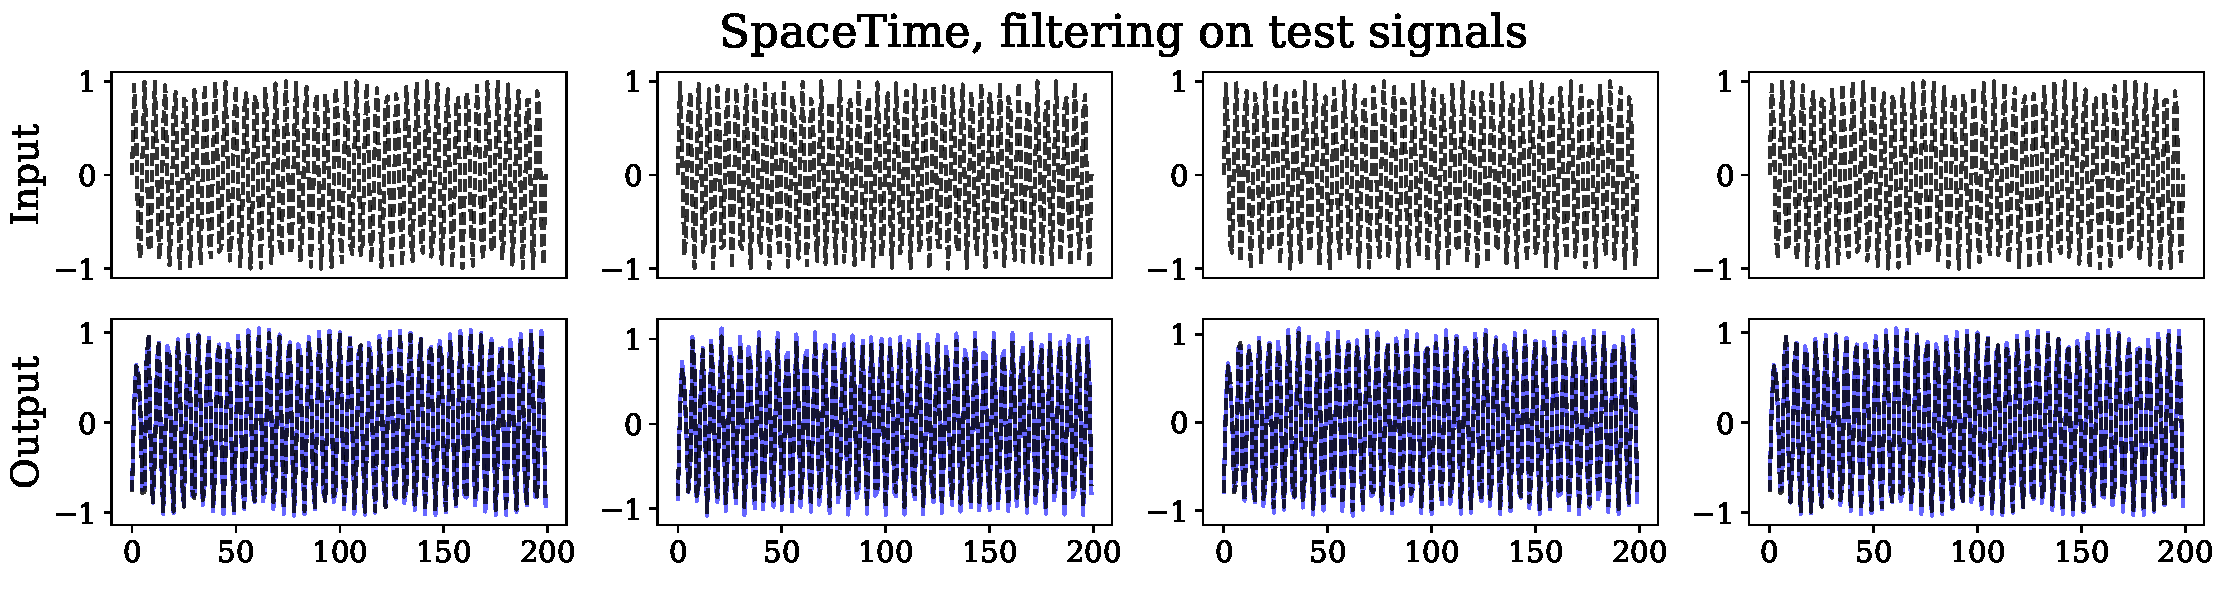
\includegraphics[scale=0.35]{_ICLR2023_paper/figures/dsp_SpaceTime.pdf}
    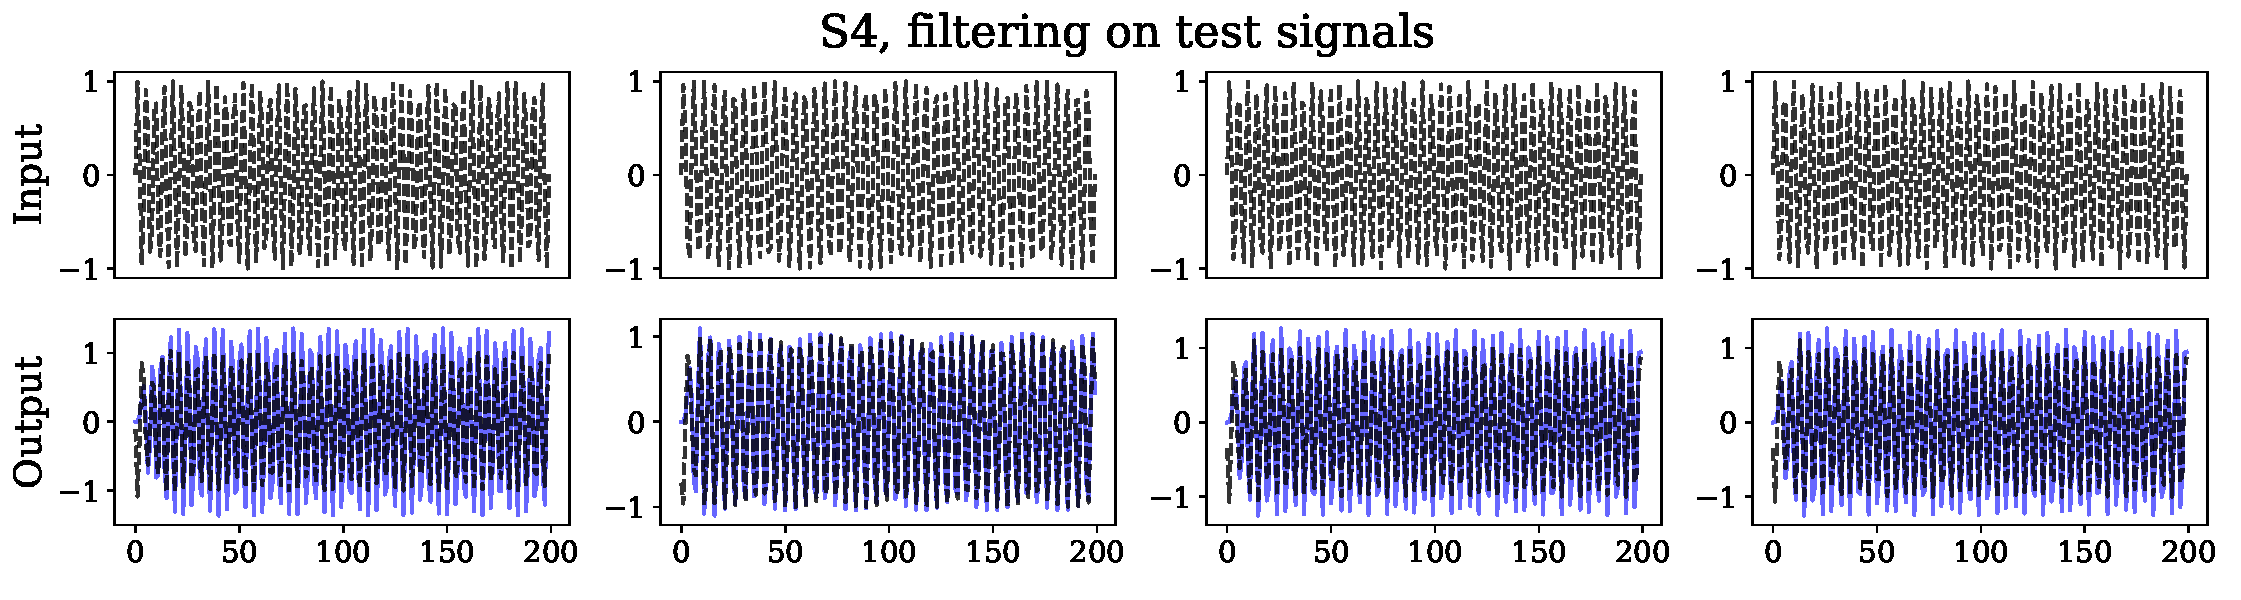
\includegraphics[scale=0.35]{_ICLR2023_paper/figures/dsp_S4.pdf}
    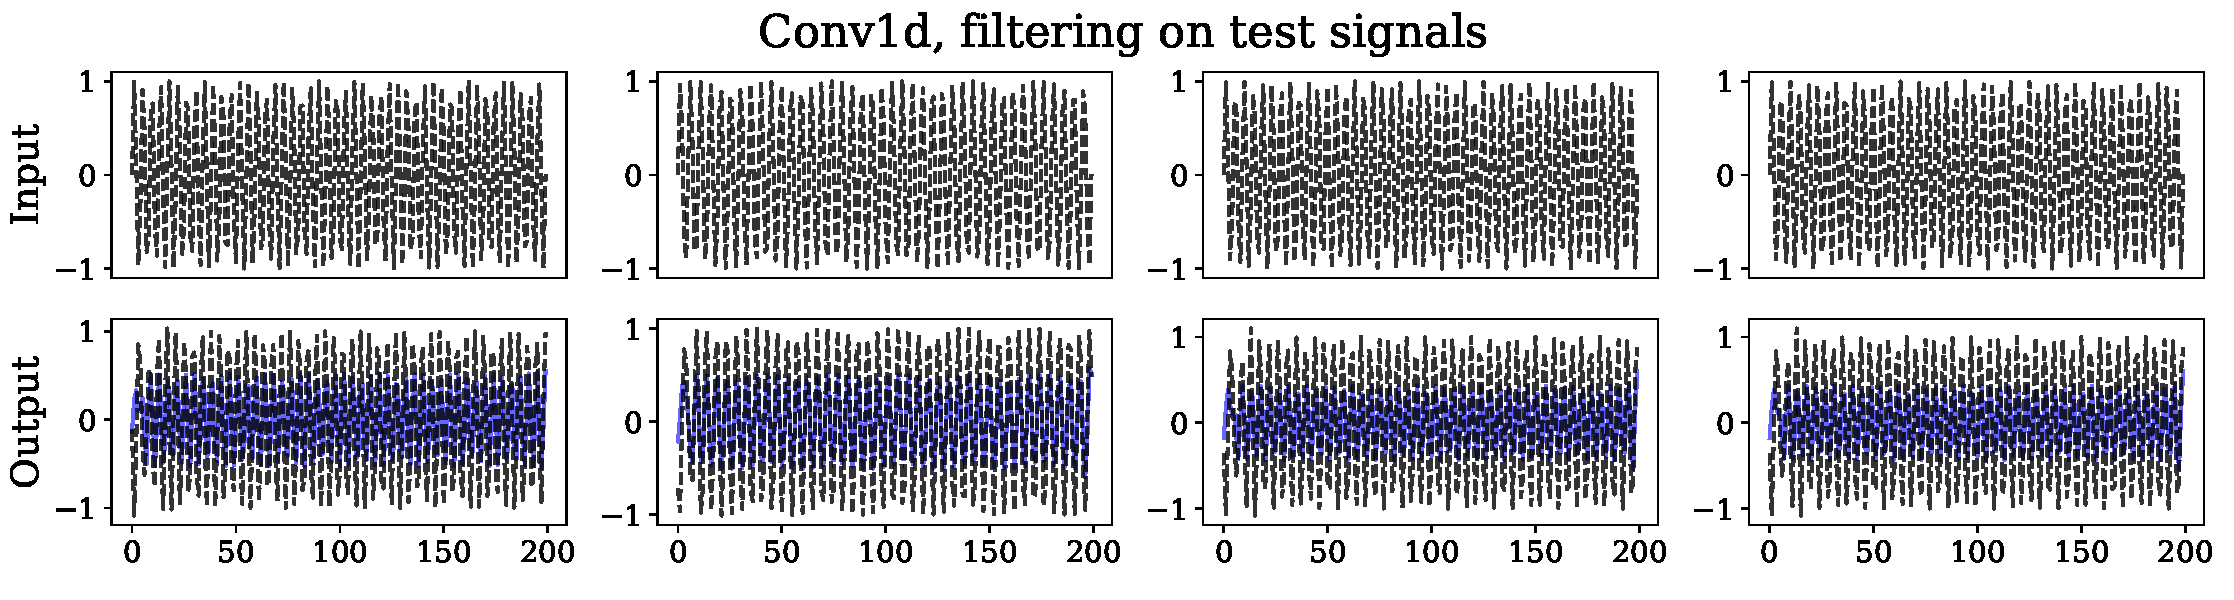
\includegraphics[scale=0.35]{_ICLR2023_paper/figures/dsp_Conv1d.pdf}
    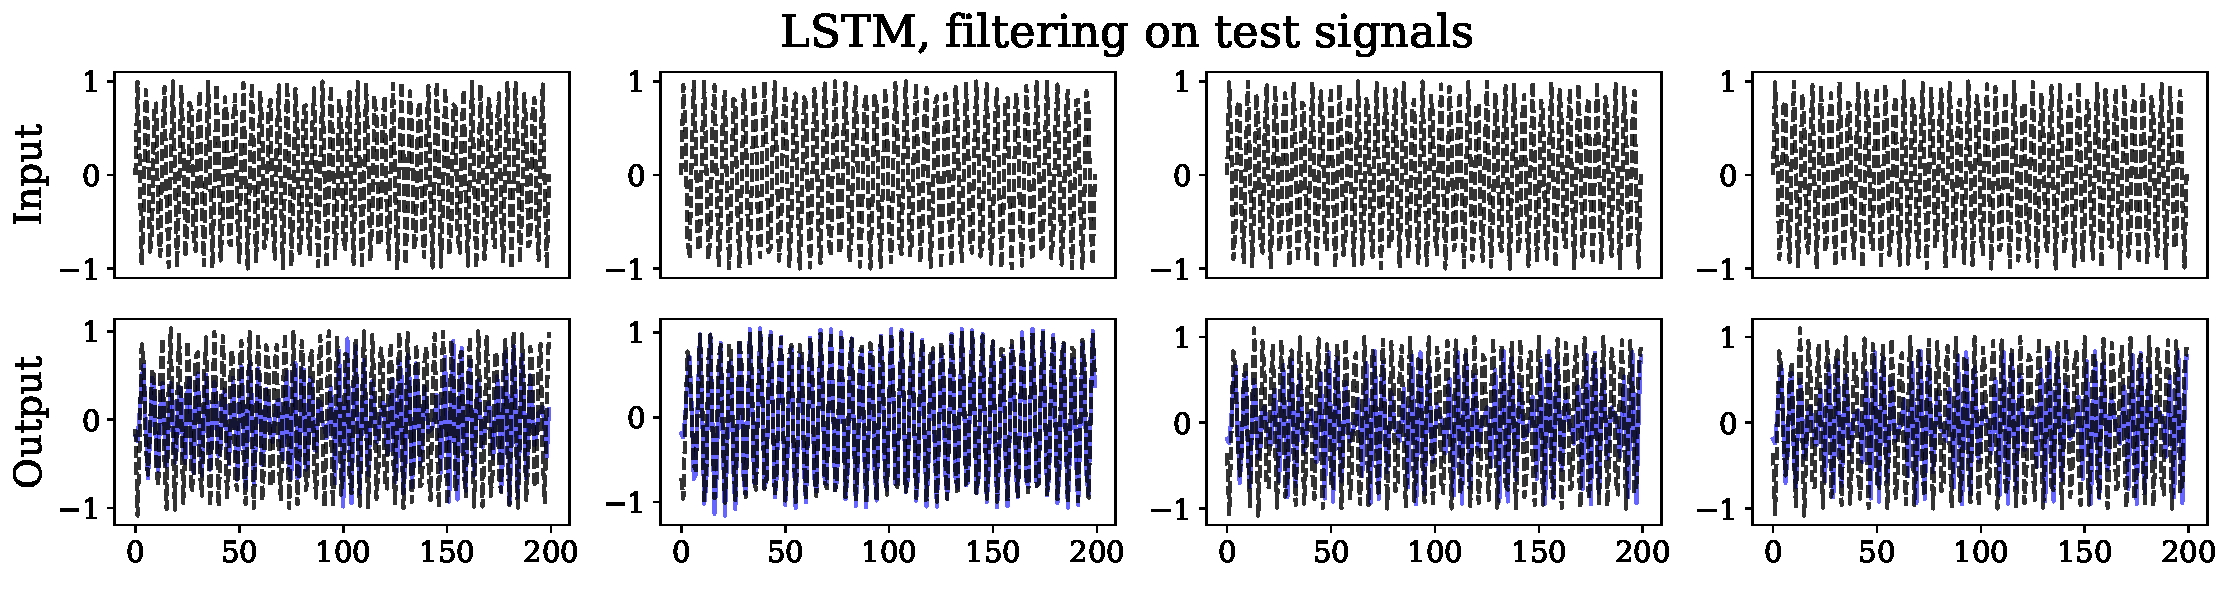
\includegraphics[scale=0.35]{_ICLR2023_paper/figures/dsp_LSTM.pdf}
    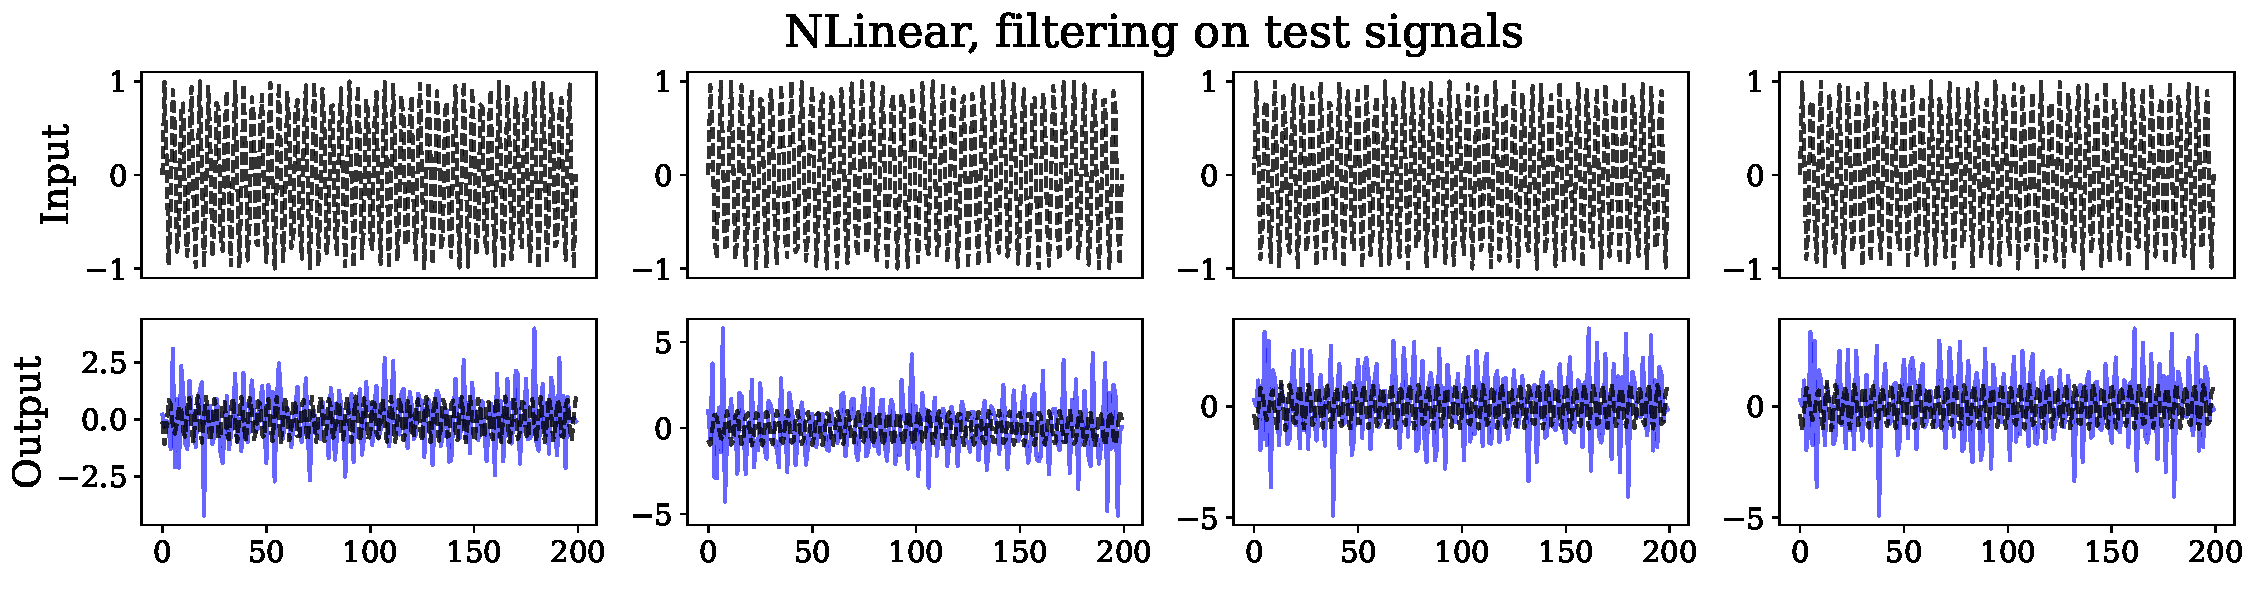
\includegraphics[scale=0.35]{_ICLR2023_paper/figures/dsp_NLinear.pdf}
    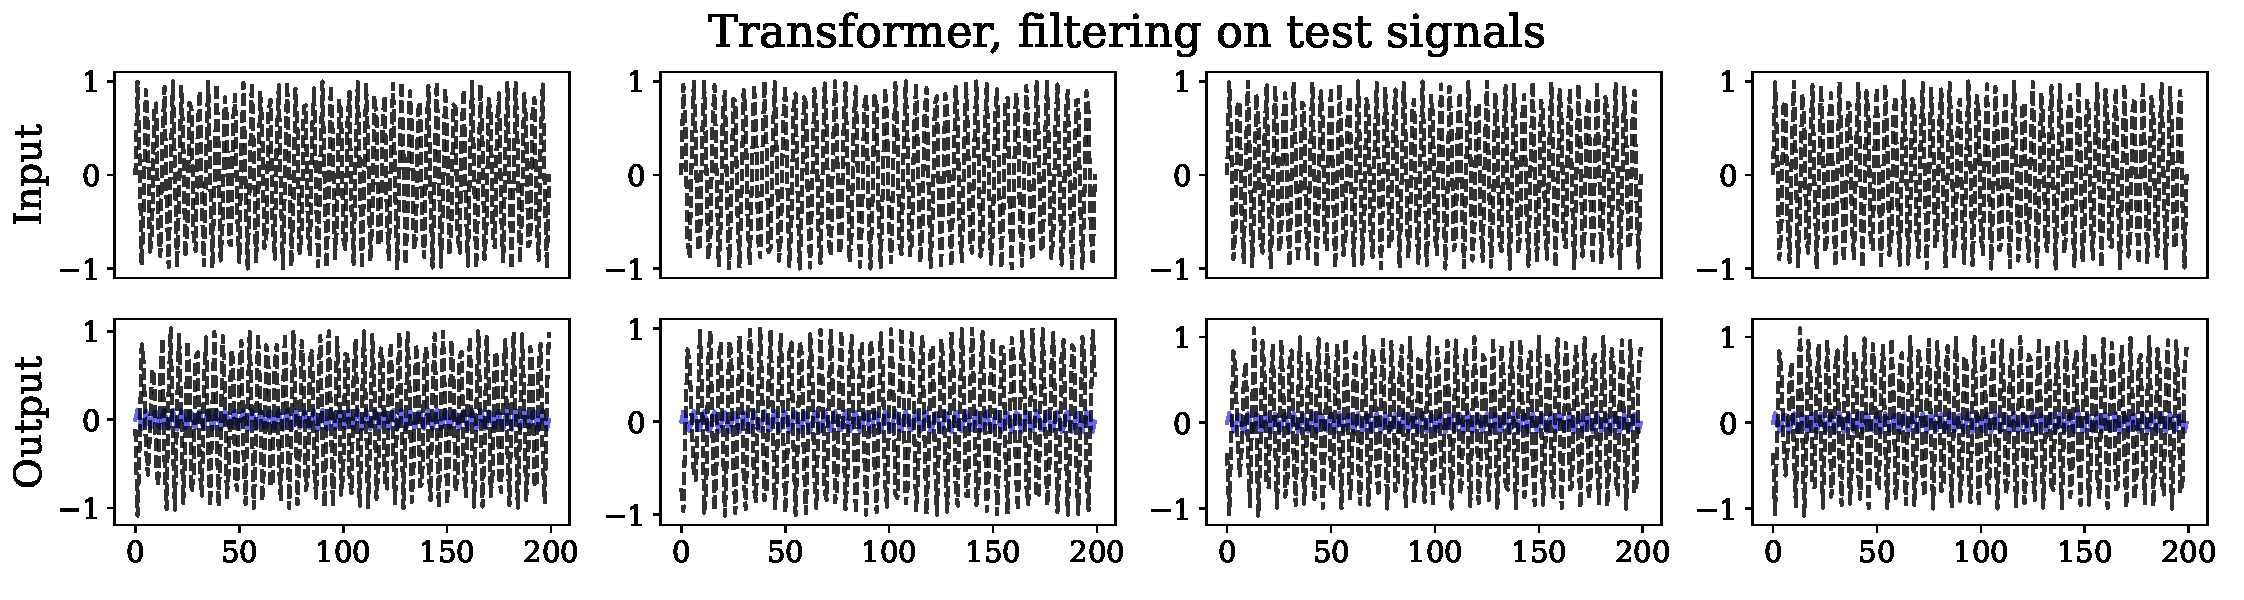
\includegraphics[scale=0.35]{_ICLR2023_paper/figures/dsp_Transformer.pdf}
    \caption{Testing the capability of different sequence--to--sequence models to approximate the input--output map of digital filters. In blue, we show the output signal filtered by each model. The ground--truth digital filter is a Butterworth of order $10$.}
    \label{fig:dsp_synthetic}
\end{figure}
%





\begin{sidewaystable}[h]
    \tiny
    \centering
    \caption{Monash forecasting. Test RMSE of \ourmethod for each dataset (best result selected via validation RMSE, average of $3$ runs).}
    \label{tab:monash}
    \begin{tabular}{c|c|cccccc|ccccc}
    \toprule
    %
    Dataset  & \ourmethod & SES & Theta & TBATS & ETS & (DHR-)ARIMA & PR & CatBoost & DeepAR & N-BEATS & WaveNet & Transformer \\
    %
    \midrule
    M1 Yearly & \underline{135508.3} & 193829.5 & 171458.1 & \textbf{116850.9} & 167739.0 & 175343.8 & 152038.7 & 237644.5 & 173075.1 & 192489.8 & 312821.8 & 182850.6 \\
    
    M1 Quarterly & \underline{2200.3} & 2545.7&	2282.7	&2673.9&	2408.5&	2538.5&	1909.3&	2161.0& 2313.3&	2267.3&	2271.7&	2231.5  \\    
    
    M1 Monthly & 2601.1 & 2725.8 & 2564.9 & 2594.5 & 2264.0 & 2450.6 & 2478.8 & 2461.7 & 2202.2 & \textbf{2183.4} & 2578.9 & 3129.8  \\

    M3 Yearly & 1412.4 & 1172.9&	1106.1&	1386.3	&1189.2	&1662.2	&1181.8&	1341.7&		1157.9&	1117.4&	1147.6&	1084.8 \\
    
    M3 Quarterly & 676.1 & 670.6&	567.7&	653.6&	598.7&	650.8&	605.5&	698.0&	606.6&	582.8&	606.8&	819.2\\ 
    
    M3 Monthly & 897.12 & 893.9	&754.0&	765.2	&755.3&	790.8&	830.0&	874.2&	873.7&	796.9&	845.3&	948.4 \\
    
    M3 Other & 265.56 & 309.7	&242.1&	217.0&	224.1	&220.8	&262.3&	349.9&	277.7&	248.5&	277.0	&271.0 \\
    
    M4 Quarterly & 718.2 & 732.8&	673.2&	672.7&	674.3&	710.0&	711.9&	714.2&	700.3&	684.7&	697.0&	739.1 \\
    
    M4 Monthly & 1092.2 & 755.5	&683.7&	743.4&	705.7&	702.1&	720.5&	734.8&	740.3&	705.2&	787.9&	902.4\\ 
    
    M4 Weekly & \textbf{348.3}& 412.6	&405.2&	356.7&	408.5	&386.3&	350.3&	420.8&	422.2&	330.8&	437.3&	456.9\\ 
    
    M4 Daily &\textbf{183.2}& 209.8&	210.4&	\underline{208.4}&	230.0	&212.6&	213.0&	263.1	&343.5&	221.7&	220.5&	233.6\\ 
    
    M4 Hourly & \textbf{255.2} & 1476.8	&1483.7	&469.9&	3830.4&	1563.1&	\underline{313.0} &	344.6&	1095.1&	501.2&	468.1&	391.2\\
    
    Tourism Yearly & \textbf{74799.2}& 106665.2&	99914.2&	105799.4&	104700.5&	106082.6&	89645.6	&87489.0&	78470.7&	78241.7	&77581.3&	80089.3\\
    
    Tourism Quarterly & 11608.32& 15000.0&	9254.6&	12001.5	&10812.3	&12564.8	&11746.9	&12788.0	&11762.0&	11306.0	&11546.6	&11724.1 \\
    
    Tourism Monthly & 3181.2& 7039.4&	2702.0	&3661.5	&2543.0	&3132.4&	2739.4&	3102.8&	2359.9&	2596.2&	2694.2&	2660.1\\
    
    Pedestrian & 69.6& 228.1&	228.2	&261.3&	278.3&	820.3&	61.8&	60.8&	65.8&	99.3&	68.0&	70.2\\
    
    Weather & \textbf{2.7}& 2.9	&3.3&	2.9&	3.0&	3.1	&9.1&	3.1&	\textbf{2.7}	&3.1&	3.0	&2.8\\
    
    NN5 Weekly & \textbf{16.9}& 18.8&	18.7&	18.5&	18.8&	18.6&	18.6&	18.7&	18.5&	17.4&	24.2&	24.0 \\
    
    Solar $10$ min &7.4& 7.2&	7.2	&10.7&	7.2	&5.6&	7.2	&8.7&	7.2	&6.6&	8.0&	7.2\\
    
    Solar Weekly &1423.7& 1331.3&	1341.6&	1049.0&	1264.4&	967.9&	1168.2&	1754.2&	873.6&	1307.8&	2569.3&	693.8\\
    
    Electricity Hourly & \textbf{475.1} & 1026.3&	1026.4&	743.4&	1524.9&	1082.4&	689.9&	582.7&	\underline{478.0} &	510.9&	489.9&	514.7\\
    
    Electricity Weekly &37802.2& 77067.9&	76935.6&	28039.7	&70369.0&	32594.8&	47802.1&	37289.7	&53100.3&	35576.8	&63916.9&	78894.7\\
    
    Fred-MD &3743.6& 3103.0&	3898.7&	2295.7&	2341.7	&3312.5&	9736.9&	2679.4&	4638.7&	2813.0&	2779.5&	5098.9\\
    
    Traffic Hourly &0.03& 0.04&	0.04	&0.05&	0.04	&0.04&	0.03	&0.03&	0.02&	0.02	&0.03&	0.02\\
    
    Traffic Weekly &\textbf{1.3}& 1.5&	1.5	&1.5&	1.5	&1.5&	1.5&	1.5	&1.5&	1.4	&1.6&	1.9\\
    
    Hospital &40.1& 26.6&	22.6&	21.3&	22.0	&23.7&	23.5&	23.5&	22.0&	24.2&	23.4&	40.5\\
    
    Covid &490.1& 403.4&	370.1&	113.0&	102.1&	100.5&	394.1&	607.9&	230.5&	186.5&	1135.4&	480.0\\
    
    Saugeen & \textbf{24.0} & 39.8	&39.8	&42.6&	50.4&	43.2&	47.7&	\underline{39.3} &	45.3&	48.9&	43.0&	49.1\\
    
    US Births &630.2& 1369.5&	735.5&	606.5&	607.2&	705.5&	732.1&	618.4&	684.0&	627.7&	768.8&	686.5\\
    
    Sunspot &3.1& 5.0	&5.0&	3.0	&5.0&	3.0	&4.0&	2.4	&1.1&	14.5&	0.7	&0.5\\
    
    Car Parts & 0.64 & 0.71&	0.65	&0.71&	0.71&	0.71&	\underline{0.58}&	0.71&	\textbf{0.50}&	1.0&	\underline{0.58}&	0.5\\
    
    Vehicle Trips &30.4& 36.5&	37.4&	25.7&	37.6&	35.0&	31.7&	27.3&	26.5&	33.6&	29.0&	33.0\\
    \bottomrule
    %
    \end{tabular}
\end{sidewaystable}

%
\end{document}